\documentclass[a4paper]{book}
\usepackage{makeidx}
\usepackage{natbib}
\usepackage{graphicx}
\usepackage{multicol}
\usepackage{float}
\usepackage{listings}
\usepackage{color}
\usepackage{ifthen}
\usepackage[table]{xcolor}
\usepackage{textcomp}
\usepackage{alltt}
\usepackage{ifpdf}
\ifpdf
\usepackage[pdftex,
            pagebackref=true,
            colorlinks=true,
            linkcolor=blue,
            unicode
           ]{hyperref}
\else
\usepackage[ps2pdf,
            pagebackref=true,
            colorlinks=true,
            linkcolor=blue,
            unicode
           ]{hyperref}
\usepackage{pspicture}
\fi
\usepackage[utf8]{inputenc}
\usepackage{mathptmx}
\usepackage[scaled=.90]{helvet}
\usepackage{courier}
\usepackage{sectsty}
\usepackage[titles]{tocloft}
\usepackage{doxygen}
\lstset{language=C++,inputencoding=utf8,basicstyle=\footnotesize,breaklines=true,breakatwhitespace=true,tabsize=4,numbers=left }
\makeindex
\setcounter{tocdepth}{3}
\renewcommand{\footrulewidth}{0.4pt}
\renewcommand{\familydefault}{\sfdefault}
\hfuzz=15pt
\setlength{\emergencystretch}{15pt}
\hbadness=750
\tolerance=750
\begin{document}
\hypersetup{pageanchor=false,citecolor=blue}
\begin{titlepage}
\vspace*{7cm}
\begin{center}
{\Large 5103 \-Project 2 }\\
\vspace*{1cm}
{\large \-Generated by Doxygen 1.7.6.1}\\
\vspace*{0.5cm}
{\small Wed Mar 28 2012 13:26:03}\\
\end{center}
\end{titlepage}
\clearemptydoublepage
\pagenumbering{roman}
\tableofcontents
\clearemptydoublepage
\pagenumbering{arabic}
\hypersetup{pageanchor=true,citecolor=blue}
\chapter{\-Class \-Index}
\section{\-Class \-Hierarchy}
\-This inheritance list is sorted roughly, but not completely, alphabetically\-:\begin{DoxyCompactList}
\item \contentsline{section}{\-Abstract\-Device}{\pageref{db/d0e/classAbstractDevice}}{}
\begin{DoxyCompactList}
\item \contentsline{section}{\-Block\-Device}{\pageref{db/d6d/classBlockDevice}}{}
\item \contentsline{section}{\-Char\-Device}{\pageref{d8/d4f/classCharDevice}}{}
\item \contentsline{section}{\-Clock\-Device}{\pageref{dc/d14/classClockDevice}}{}
\end{DoxyCompactList}
\item \contentsline{section}{c\-C\-P\-U}{\pageref{d2/dc6/classcCPU}}{}
\item \contentsline{section}{c\-I\-D\-Manager}{\pageref{de/dd4/classcIDManager}}{}
\item \contentsline{section}{c\-Kernel}{\pageref{db/da5/classcKernel}}{}
\item \contentsline{section}{c\-Round\-Robin}{\pageref{dc/dcc/classcRoundRobin}}{}
\item \contentsline{section}{c\-Scheduler}{\pageref{d0/d21/classcScheduler}}{}
\begin{DoxyCompactList}
\item \contentsline{section}{c\-F\-C\-F\-S}{\pageref{d6/dc3/classcFCFS}}{}
\end{DoxyCompactList}
\item \contentsline{section}{fcfs\-Info}{\pageref{d5/d4c/structfcfsInfo}}{}
\item \contentsline{section}{kernel\-Error}{\pageref{dc/d4b/structkernelError}}{}
\item \contentsline{section}{\-Process\-Info}{\pageref{dd/dc8/structProcessInfo}}{}
\end{DoxyCompactList}

\chapter{\-Class \-Index}
\section{\-Class \-List}
\-Here are the classes, structs, unions and interfaces with brief descriptions\-:\begin{DoxyCompactList}
\item\contentsline{section}{\hyperlink{classAbstractDevice}{\-Abstract\-Device} }{\pageref{db/d0e/classAbstractDevice}}{}
\item\contentsline{section}{\hyperlink{classBlockDevice}{\-Block\-Device} }{\pageref{db/d6d/classBlockDevice}}{}
\item\contentsline{section}{\hyperlink{classcCPU}{c\-C\-P\-U} \\*\-A class for emulating a simple cpu }{\pageref{d2/dc6/classcCPU}}{}
\item\contentsline{section}{\hyperlink{classcFCFS}{c\-F\-C\-F\-S} }{\pageref{d6/dc3/classcFCFS}}{}
\item\contentsline{section}{\hyperlink{classCharDevice}{\-Char\-Device} }{\pageref{d8/d4f/classCharDevice}}{}
\item\contentsline{section}{\hyperlink{classcIDManager}{c\-I\-D\-Manager} }{\pageref{de/dd4/classcIDManager}}{}
\item\contentsline{section}{\hyperlink{classcKernel}{c\-Kernel} }{\pageref{db/da5/classcKernel}}{}
\item\contentsline{section}{\hyperlink{classClockDevice}{\-Clock\-Device} }{\pageref{dc/d14/classClockDevice}}{}
\item\contentsline{section}{\hyperlink{classcScheduler}{c\-Scheduler} }{\pageref{d0/d21/classcScheduler}}{}
\item\contentsline{section}{\hyperlink{structProcessInfo}{\-Process\-Info} \\*\-Structure for containing process state and data }{\pageref{dd/dc8/structProcessInfo}}{}
\end{DoxyCompactList}

\chapter{\-File \-Index}
\section{\-File \-List}
\-Here is a list of all documented files with brief descriptions\-:\begin{DoxyCompactList}
\item\contentsline{section}{include/\hyperlink{cpu_8h}{cpu.\-h} }{\pageref{dc/da7/cpu_8h}}{}
\item\contentsline{section}{include/{\bfseries init.\-h} }{\pageref{d8/dc0/init_8h}}{}
\item\contentsline{section}{include/{\bfseries kernel.\-h} }{\pageref{d0/daa/kernel_8h}}{}
\item\contentsline{section}{include/{\bfseries process.\-h} }{\pageref{da/d42/process_8h}}{}
\item\contentsline{section}{include/devices/{\bfseries abstract\-\_\-device.\-h} }{\pageref{d0/d8f/abstract__device_8h}}{}
\item\contentsline{section}{include/devices/{\bfseries block\-\_\-device.\-h} }{\pageref{db/d9a/block__device_8h}}{}
\item\contentsline{section}{include/devices/{\bfseries char\-\_\-device.\-h} }{\pageref{d7/d59/char__device_8h}}{}
\item\contentsline{section}{include/devices/{\bfseries clock\-\_\-device.\-h} }{\pageref{df/d8f/clock__device_8h}}{}
\item\contentsline{section}{include/scheduler/{\bfseries fcfs.\-h} }{\pageref{db/d41/fcfs_8h}}{}
\item\contentsline{section}{include/scheduler/{\bfseries scheduler.\-h} }{\pageref{d2/dd8/scheduler_8h}}{}
\item\contentsline{section}{include/utility/{\bfseries id.\-h} }{\pageref{df/db9/id_8h}}{}
\end{DoxyCompactList}

\chapter{\-Class \-Documentation}
\hypertarget{classcCleanDaemon}{\section{c\-Clean\-Daemon \-Class \-Reference}
\label{d3/d6f/classcCleanDaemon}\index{c\-Clean\-Daemon@{c\-Clean\-Daemon}}
}


\-Cleaning \-Daemon for system.  




{\ttfamily \#include $<$cleaning\-Daemon.\-h$>$}



\-Collaboration diagram for c\-Clean\-Daemon\-:\nopagebreak
\begin{figure}[H]
\begin{center}
\leavevmode
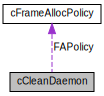
\includegraphics[width=176pt]{d7/def/classcCleanDaemon__coll__graph}
\end{center}
\end{figure}
\subsection*{\-Public \-Member \-Functions}
\begin{DoxyCompactItemize}
\item 
\hypertarget{classcCleanDaemon_a7646bbaebfefa0c9478e5a23333768db}{{\bfseries c\-Clean\-Daemon} (\hyperlink{classcFrameAllocPolicy}{c\-Frame\-Alloc\-Policy} \&\-\_\-\-F\-A)}\label{d3/d6f/classcCleanDaemon_a7646bbaebfefa0c9478e5a23333768db}

\item 
uint32\-\_\-t \hyperlink{classcCleanDaemon_ac9a8ca1ac1d35f554af393274dd87f68}{check\-Clean} ()
\begin{DoxyCompactList}\small\item\em \-Check if pages need to be cleaned. \end{DoxyCompactList}\end{DoxyCompactItemize}
\subsection*{\-Private \-Attributes}
\begin{DoxyCompactItemize}
\item 
\hypertarget{classcCleanDaemon_a175b113f2f0f943199348e7f1f55252e}{\hyperlink{classcFrameAllocPolicy}{c\-Frame\-Alloc\-Policy} \& {\bfseries \-F\-A\-Policy}}\label{d3/d6f/classcCleanDaemon_a175b113f2f0f943199348e7f1f55252e}

\item 
\hypertarget{classcCleanDaemon_aa02439f18adb8dc65b2595eb7ae99158}{uint32\-\_\-t {\bfseries min\-\_\-thresh}}\label{d3/d6f/classcCleanDaemon_aa02439f18adb8dc65b2595eb7ae99158}

\item 
\hypertarget{classcCleanDaemon_af193b6bcae4c81485b62cba8c413c7ab}{uint32\-\_\-t {\bfseries clean\-\_\-amnt}}\label{d3/d6f/classcCleanDaemon_af193b6bcae4c81485b62cba8c413c7ab}

\end{DoxyCompactItemize}


\subsection{\-Member \-Function \-Documentation}
\hypertarget{classcCleanDaemon_ac9a8ca1ac1d35f554af393274dd87f68}{\index{c\-Clean\-Daemon@{c\-Clean\-Daemon}!check\-Clean@{check\-Clean}}
\index{check\-Clean@{check\-Clean}!cCleanDaemon@{c\-Clean\-Daemon}}
\subsubsection[{check\-Clean}]{\setlength{\rightskip}{0pt plus 5cm}uint32\-\_\-t {\bf c\-Clean\-Daemon\-::check\-Clean} (
\begin{DoxyParamCaption}
{}
\end{DoxyParamCaption}
)}}\label{d3/d6f/classcCleanDaemon_ac9a8ca1ac1d35f554af393274dd87f68}
\-The \-V\-M\-M core calls this and the daemon checks with the \-F\-A module to see how many frames are available. \-If it is below its threshold it returns how many should be cleaned. \-This value is passed to the \-P\-R module which makes the policy decisions on which to replace. 

\-Referenced by c\-V\-M\-M\-::start().



\-The documentation for this class was generated from the following files\-:\begin{DoxyCompactItemize}
\item 
include/\-Policy/\hyperlink{cleaningDaemon_8h}{cleaning\-Daemon.\-h}\item 
src/\-Policy/cleaning\-Daemon.\-cpp\end{DoxyCompactItemize}

\hypertarget{classcCPU}{\section{c\-C\-P\-U \-Class \-Reference}
\label{d2/dc6/classcCPU}\index{c\-C\-P\-U@{c\-C\-P\-U}}
}


{\ttfamily \#include $<$cpu.\-h$>$}

\subsection*{\-Public \-Member \-Functions}
\begin{DoxyCompactItemize}
\item 
void \hyperlink{classcCPU_acd957640be8abb7c0d8a24010ed0e737}{set\-Text} (char $\ast$text)
\item 
unsigned int \hyperlink{classcCPU_ab04938ac939d530e521181db6a52944f}{get\-Set\-P\-C} (unsigned int new\-P\-C)
\item 
int \hyperlink{classcCPU_a2d593a0d3d66e532826db4754d5fc4d2}{get\-Set\-V\-C} (int new\-V\-C)
\item 
uint16\-\_\-t \hyperlink{classcCPU_ad485374a709476e2dfb847046d3d5215}{get\-P\-S\-W} ()
\item 
char $\ast$ \hyperlink{classcCPU_a891d9b77e1818ca247e9d76f4db99415}{get\-Param} (int num)
\item 
char \hyperlink{classcCPU_a987e1ab511c71dcde48411f5bb16f9d8}{get\-Opcode} ()
\item 
void \hyperlink{classcCPU_aee300d68026ba9f13d5434ff82f0372a}{run} ()
\end{DoxyCompactItemize}


\subsection{\-Detailed \-Description}
\-A class for emulating a simple cpu.

\-This class emulates the internals of a very simple cpu with two main registers, \-P\-C and \-V\-C. \-In addition, it has other state for handling system calls and program exceptions. 

\subsection{\-Member \-Function \-Documentation}
\hypertarget{classcCPU_a987e1ab511c71dcde48411f5bb16f9d8}{\index{c\-C\-P\-U@{c\-C\-P\-U}!get\-Opcode@{get\-Opcode}}
\index{get\-Opcode@{get\-Opcode}!cCPU@{c\-C\-P\-U}}
\subsubsection[{get\-Opcode}]{\setlength{\rightskip}{0pt plus 5cm}char {\bf c\-C\-P\-U\-::get\-Opcode} (
\begin{DoxyParamCaption}
{}
\end{DoxyParamCaption}
)}}\label{d2/dc6/classcCPU_a987e1ab511c71dcde48411f5bb16f9d8}
\-Get the current \-Opcode

\-Get the current \-Opcode in the cpu. \-This is used by the kernel to determine which system call as being made. \-Used in conjunciton with \hyperlink{classcCPU_a891d9b77e1818ca247e9d76f4db99415}{c\-C\-P\-U\-::get\-Param} the kernel can process system calls. \hypertarget{classcCPU_a891d9b77e1818ca247e9d76f4db99415}{\index{c\-C\-P\-U@{c\-C\-P\-U}!get\-Param@{get\-Param}}
\index{get\-Param@{get\-Param}!cCPU@{c\-C\-P\-U}}
\subsubsection[{get\-Param}]{\setlength{\rightskip}{0pt plus 5cm}char $\ast$ {\bf c\-C\-P\-U\-::get\-Param} (
\begin{DoxyParamCaption}
\item[{int}]{num}
\end{DoxyParamCaption}
)}}\label{d2/dc6/classcCPU_a891d9b77e1818ca247e9d76f4db99415}
\-Get execution parameters from the cpu

\-Fetch the given execution paramter from the cpu's internal buffer. \-When an instruction is encountered that has parameters associated with it, the cpu tokenizes them and places it in an internal buffer. \-This function is mainly used by the kernel in handling system calls.


\begin{DoxyParams}{\-Parameters}
{\em num} & \-Must be less than \-M\-A\-X\-\_\-\-P\-A\-R\-A\-M\-S (currently 2)\\
\hline
\end{DoxyParams}
\begin{DoxyReturn}{\-Returns}
\-Returns a char$\ast$ which points to a string of at most \-M\-A\-X\-\_\-\-P\-A\-R\-A\-M\-\_\-\-S\-I\-Z\-E -\/ 1 bytes. 
\end{DoxyReturn}
\hypertarget{classcCPU_ad485374a709476e2dfb847046d3d5215}{\index{c\-C\-P\-U@{c\-C\-P\-U}!get\-P\-S\-W@{get\-P\-S\-W}}
\index{get\-P\-S\-W@{get\-P\-S\-W}!cCPU@{c\-C\-P\-U}}
\subsubsection[{get\-P\-S\-W}]{\setlength{\rightskip}{0pt plus 5cm}uint16\-\_\-t {\bf c\-C\-P\-U\-::get\-P\-S\-W} (
\begin{DoxyParamCaption}
{}
\end{DoxyParamCaption}
)}}\label{d2/dc6/classcCPU_ad485374a709476e2dfb847046d3d5215}
\-Get the \-Program \-Status \-Word

\-Returns the program status word which is a unsigned 16-\/bit integer type with flags from \hyperlink{cpu_8h_ade10811b11f1c647313bf0a60797a9f9}{e\-P\-S\-W} set. \-These are used by the kernel to make action decisions. \hypertarget{classcCPU_ab04938ac939d530e521181db6a52944f}{\index{c\-C\-P\-U@{c\-C\-P\-U}!get\-Set\-P\-C@{get\-Set\-P\-C}}
\index{get\-Set\-P\-C@{get\-Set\-P\-C}!cCPU@{c\-C\-P\-U}}
\subsubsection[{get\-Set\-P\-C}]{\setlength{\rightskip}{0pt plus 5cm}unsigned int {\bf c\-C\-P\-U\-::get\-Set\-P\-C} (
\begin{DoxyParamCaption}
\item[{unsigned int}]{new\-P\-C}
\end{DoxyParamCaption}
)}}\label{d2/dc6/classcCPU_ab04938ac939d530e521181db6a52944f}
\-Get/\-Set the program counter

\-Get the current value for the program counter and then set its value to the given parameter. \-This is useful for swapping out process values. \hypertarget{classcCPU_a2d593a0d3d66e532826db4754d5fc4d2}{\index{c\-C\-P\-U@{c\-C\-P\-U}!get\-Set\-V\-C@{get\-Set\-V\-C}}
\index{get\-Set\-V\-C@{get\-Set\-V\-C}!cCPU@{c\-C\-P\-U}}
\subsubsection[{get\-Set\-V\-C}]{\setlength{\rightskip}{0pt plus 5cm}int {\bf c\-C\-P\-U\-::get\-Set\-V\-C} (
\begin{DoxyParamCaption}
\item[{int}]{new\-V\-C}
\end{DoxyParamCaption}
)}}\label{d2/dc6/classcCPU_a2d593a0d3d66e532826db4754d5fc4d2}
\-Get/\-Set the \-V\-C

\-Get the current value for \-V\-C and set its value to the given paramter. \-This is useful for swapping out process values. \hypertarget{classcCPU_aee300d68026ba9f13d5434ff82f0372a}{\index{c\-C\-P\-U@{c\-C\-P\-U}!run@{run}}
\index{run@{run}!cCPU@{c\-C\-P\-U}}
\subsubsection[{run}]{\setlength{\rightskip}{0pt plus 5cm}void {\bf c\-C\-P\-U\-::run} (
\begin{DoxyParamCaption}
{}
\end{DoxyParamCaption}
)}}\label{d2/dc6/classcCPU_aee300d68026ba9f13d5434ff82f0372a}
\-Start execution

\-Once all appropriate process data is entered by the kernel this function is called to start execution. \-Any time control needs to be returned to the kernel this function will return with the appropriate \-P\-S\-W flags set for the kernel to act on. \hypertarget{classcCPU_acd957640be8abb7c0d8a24010ed0e737}{\index{c\-C\-P\-U@{c\-C\-P\-U}!set\-Text@{set\-Text}}
\index{set\-Text@{set\-Text}!cCPU@{c\-C\-P\-U}}
\subsubsection[{set\-Text}]{\setlength{\rightskip}{0pt plus 5cm}void {\bf c\-C\-P\-U\-::set\-Text} (
\begin{DoxyParamCaption}
\item[{char $\ast$}]{text}
\end{DoxyParamCaption}
)}}\label{d2/dc6/classcCPU_acd957640be8abb7c0d8a24010ed0e737}
\-Set the program text

\-Point the cpu to the text data for the running process. \-This text is indexed using the program counter (\-P\-C).


\begin{DoxyParams}{\-Parameters}
{\em text} & \-Program text pointer. assert( text != \-N\-U\-L\-L) \\
\hline
\end{DoxyParams}


\-The documentation for this class was generated from the following files\-:\begin{DoxyCompactItemize}
\item 
include/\hyperlink{cpu_8h}{cpu.\-h}\item 
src/cpu.\-cpp\end{DoxyCompactItemize}

\hypertarget{classcException}{\section{c\-Exception \-Class \-Reference}
\label{d3/d42/classcException}\index{c\-Exception@{c\-Exception}}
}


\-Generic exception class.  




{\ttfamily \#include $<$exceptions.\-h$>$}



\-Inheritance diagram for c\-Exception\-:\nopagebreak
\begin{figure}[H]
\begin{center}
\leavevmode
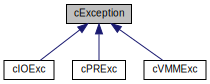
\includegraphics[width=282pt]{d8/d8b/classcException__inherit__graph}
\end{center}
\end{figure}
\subsection*{\-Public \-Member \-Functions}
\begin{DoxyCompactItemize}
\item 
\hypertarget{classcException_acfea75107323730d40fb9c51d1283db4}{void {\bfseries set\-Error\-Str} (const string \&msg)}\label{d3/d42/classcException_acfea75107323730d40fb9c51d1283db4}

\item 
void \hyperlink{classcException_a8b5b59765cea5af7c827399d07b0b47e}{set\-Fatality} (bool f)
\begin{DoxyCompactList}\small\item\em \-Is this a fatal error? \end{DoxyCompactList}\item 
\hypertarget{classcException_aa51695c5454c316f6beed190b6fa5a22}{string \& {\bfseries get\-Error\-Str} ()}\label{d3/d42/classcException_aa51695c5454c316f6beed190b6fa5a22}

\item 
\hypertarget{classcException_a2c75c6b63164915792b867b673e451a3}{bool {\bfseries is\-Fatal} ()}\label{d3/d42/classcException_a2c75c6b63164915792b867b673e451a3}

\end{DoxyCompactItemize}
\subsection*{\-Private \-Attributes}
\begin{DoxyCompactItemize}
\item 
\hypertarget{classcException_a52fe1ef0b911901eaf6d24226c99ad51}{string {\bfseries err\-Msg}}\label{d3/d42/classcException_a52fe1ef0b911901eaf6d24226c99ad51}

\item 
\hypertarget{classcException_af2378417da8ced98712165bbbb3a31de}{bool {\bfseries fatal}}\label{d3/d42/classcException_af2378417da8ced98712165bbbb3a31de}

\end{DoxyCompactItemize}


\subsection{\-Detailed \-Description}
\-These exceptions are caught in main and their error messages are printed out. 

\subsection{\-Member \-Function \-Documentation}
\hypertarget{classcException_a8b5b59765cea5af7c827399d07b0b47e}{\index{c\-Exception@{c\-Exception}!set\-Fatality@{set\-Fatality}}
\index{set\-Fatality@{set\-Fatality}!cException@{c\-Exception}}
\subsubsection[{set\-Fatality}]{\setlength{\rightskip}{0pt plus 5cm}void {\bf c\-Exception\-::set\-Fatality} (
\begin{DoxyParamCaption}
\item[{bool}]{f}
\end{DoxyParamCaption}
)\hspace{0.3cm}{\ttfamily  \mbox{[}inline\mbox{]}}}}\label{d3/d42/classcException_a8b5b59765cea5af7c827399d07b0b47e}
\-After this is set you must press up, up, down, down, left, right, left, right, \-B, \-A. \-Hopefully then the program will fix itself. \-No really, you should end the program. 

\-Referenced by c\-P\-R\-Fifo\-::clear\-Pages(), c\-P\-R\-Lru\-Approx\-::clear\-Pages(), and c\-P\-R\-Lru\-::clear\-Pages().



\-The documentation for this class was generated from the following file\-:\begin{DoxyCompactItemize}
\item 
include/\hyperlink{exceptions_8h}{exceptions.\-h}\end{DoxyCompactItemize}

\hypertarget{classcFixedAlloc}{\section{c\-Fixed\-Alloc \-Class \-Reference}
\label{d1/d40/classcFixedAlloc}\index{c\-Fixed\-Alloc@{c\-Fixed\-Alloc}}
}


\-Inheritance diagram for c\-Fixed\-Alloc\-:\nopagebreak
\begin{figure}[H]
\begin{center}
\leavevmode
\includegraphics[width=176pt]{dc/d13/classcFixedAlloc__inherit__graph}
\end{center}
\end{figure}


\-Collaboration diagram for c\-Fixed\-Alloc\-:\nopagebreak
\begin{figure}[H]
\begin{center}
\leavevmode
\includegraphics[width=176pt]{d4/d27/classcFixedAlloc__coll__graph}
\end{center}
\end{figure}
\subsection*{\-Public \-Member \-Functions}
\begin{DoxyCompactItemize}
\item 
void \hyperlink{classcFixedAlloc_a489395f063815020f36265a52308a3f6}{reg\-Procs} (vector$<$ \hyperlink{structsProc}{s\-Proc} $\ast$ $>$ \&procs)
\begin{DoxyCompactList}\small\item\em \-Give the policy module information about processes. \end{DoxyCompactList}\item 
\hypertarget{classcFixedAlloc_a12285e88707a40ae51b5d2963dfea1aa}{bool {\bfseries check\-Available} (uint32\-\_\-t frame, bool pinned\-Taken=true)}\label{d1/d40/classcFixedAlloc_a12285e88707a40ae51b5d2963dfea1aa}

\item 
\hypertarget{classcFixedAlloc_a6a9ece4fe93de1473efe111d44830cd1}{pair$<$ bool, uint32\-\_\-t $>$ {\bfseries get\-Frame} ()}\label{d1/d40/classcFixedAlloc_a6a9ece4fe93de1473efe111d44830cd1}

\item 
\hypertarget{classcFixedAlloc_acc3148cce2f2880af5624c2a409eafb4}{pair$<$ bool, uint32\-\_\-t $>$ {\bfseries get\-Frame} (\hyperlink{structsProc}{s\-Proc} $\ast$)}\label{d1/d40/classcFixedAlloc_acc3148cce2f2880af5624c2a409eafb4}

\item 
\hypertarget{classcFixedAlloc_ad51c52d37f59f8a40eb315f35892bc98}{bool {\bfseries get\-Frame} (uint32\-\_\-t frame)}\label{d1/d40/classcFixedAlloc_ad51c52d37f59f8a40eb315f35892bc98}

\item 
void \hyperlink{classcFixedAlloc_a79df79853a015bb750ca682630afcfd8}{return\-Frame} (uint32\-\_\-t frame)
\begin{DoxyCompactList}\small\item\em \-System is returning a page. \end{DoxyCompactList}\item 
\hypertarget{classcFixedAlloc_a2109057465d037b0c23dba1257163aba}{uint32\-\_\-t {\bfseries check\-Open} (bool)}\label{d1/d40/classcFixedAlloc_a2109057465d037b0c23dba1257163aba}

\item 
\hypertarget{classcFixedAlloc_a0baba5ee9e04148d9d5845ee5afbfe37}{bool {\bfseries pin} (uint32\-\_\-t frame)}\label{d1/d40/classcFixedAlloc_a0baba5ee9e04148d9d5845ee5afbfe37}

\item 
\hypertarget{classcFixedAlloc_a2a6f869ad3c6fa6190fdbca3e198bae9}{bool {\bfseries unpin} (uint32\-\_\-t frame)}\label{d1/d40/classcFixedAlloc_a2a6f869ad3c6fa6190fdbca3e198bae9}

\end{DoxyCompactItemize}
\subsection*{\-Private \-Member \-Functions}
\begin{DoxyCompactItemize}
\item 
\hypertarget{classcFixedAlloc_ad7bb774118a2d337f8f5f950c22b7ee0}{uint32\-\_\-t {\bfseries find\-First\-Of} (bool check, dynamic\-\_\-bitset$<$$>$ \&bits)}\label{d1/d40/classcFixedAlloc_ad7bb774118a2d337f8f5f950c22b7ee0}

\item 
\hypertarget{classcFixedAlloc_a14dda43745a14f32f5e01b37797ac879}{void {\bfseries print\-Frames} ()}\label{d1/d40/classcFixedAlloc_a14dda43745a14f32f5e01b37797ac879}

\end{DoxyCompactItemize}
\subsection*{\-Private \-Attributes}
\begin{DoxyCompactItemize}
\item 
\hypertarget{classcFixedAlloc_aaf24339f1c79274e4d24fb1044d6ed25}{int {\bfseries alloc\-Size}}\label{d1/d40/classcFixedAlloc_aaf24339f1c79274e4d24fb1044d6ed25}

\item 
\hypertarget{classcFixedAlloc_a7df629e87072fd179c7e7934d2424815}{dynamic\-\_\-bitset {\bfseries frames}}\label{d1/d40/classcFixedAlloc_a7df629e87072fd179c7e7934d2424815}

\item 
\hypertarget{classcFixedAlloc_a09c47ddabbcc2e8f8708c929fefff05b}{dynamic\-\_\-bitset {\bfseries pinned}}\label{d1/d40/classcFixedAlloc_a09c47ddabbcc2e8f8708c929fefff05b}

\item 
\hypertarget{classcFixedAlloc_a369c2714b4308ef100b81195ead0b24a}{uint32\-\_\-t {\bfseries num\-Frames}}\label{d1/d40/classcFixedAlloc_a369c2714b4308ef100b81195ead0b24a}

\item 
\hypertarget{classcFixedAlloc_aed0c422265af0f1c248c6a5f4b6336d9}{uint32\-\_\-t {\bfseries open\-Frames}}\label{d1/d40/classcFixedAlloc_aed0c422265af0f1c248c6a5f4b6336d9}

\item 
\hypertarget{classcFixedAlloc_aeb96768ba92b2d27f3c736fed35076e2}{bool {\bfseries \-\_\-print\-F}}\label{d1/d40/classcFixedAlloc_aeb96768ba92b2d27f3c736fed35076e2}

\item 
\hypertarget{classcFixedAlloc_a619d729276b056675bc582b406f5d385}{bool {\bfseries \-\_\-print\-F\-\_\-on\-\_\-pin}}\label{d1/d40/classcFixedAlloc_a619d729276b056675bc582b406f5d385}

\item 
\hypertarget{classcFixedAlloc_ad953ea8614b03e098d3e46a6087e15ba}{\-F\-I\-L\-E $\ast$ {\bfseries print\-Loc}}\label{d1/d40/classcFixedAlloc_ad953ea8614b03e098d3e46a6087e15ba}

\end{DoxyCompactItemize}


\subsection{\-Member \-Function \-Documentation}
\hypertarget{classcFixedAlloc_a489395f063815020f36265a52308a3f6}{\index{c\-Fixed\-Alloc@{c\-Fixed\-Alloc}!reg\-Procs@{reg\-Procs}}
\index{reg\-Procs@{reg\-Procs}!cFixedAlloc@{c\-Fixed\-Alloc}}
\subsubsection[{reg\-Procs}]{\setlength{\rightskip}{0pt plus 5cm}void {\bf c\-Fixed\-Alloc\-::reg\-Procs} (
\begin{DoxyParamCaption}
\item[{vector$<$ {\bf s\-Proc} $\ast$ $>$ \&}]{procs}
\end{DoxyParamCaption}
)\hspace{0.3cm}{\ttfamily  \mbox{[}virtual\mbox{]}}}}\label{d1/d40/classcFixedAlloc_a489395f063815020f36265a52308a3f6}
\-Some frame allocation policies may want information regarding particular processes. \-This is called after construction and it gives the policy a chance to build any necessary datastructures. 

\-Implements \hyperlink{classcFrameAllocPolicy_a84e52441bcbb0a571bbcf1a7209cd662}{c\-Frame\-Alloc\-Policy}.

\hypertarget{classcFixedAlloc_a79df79853a015bb750ca682630afcfd8}{\index{c\-Fixed\-Alloc@{c\-Fixed\-Alloc}!return\-Frame@{return\-Frame}}
\index{return\-Frame@{return\-Frame}!cFixedAlloc@{c\-Fixed\-Alloc}}
\subsubsection[{return\-Frame}]{\setlength{\rightskip}{0pt plus 5cm}void {\bf c\-Fixed\-Alloc\-::return\-Frame} (
\begin{DoxyParamCaption}
\item[{uint32\-\_\-t}]{frame}
\end{DoxyParamCaption}
)\hspace{0.3cm}{\ttfamily  \mbox{[}virtual\mbox{]}}}}\label{d1/d40/classcFixedAlloc_a79df79853a015bb750ca682630afcfd8}
\-This could happen on process termination or invocation of the page cleaning daemon. 

\-Implements \hyperlink{classcFrameAllocPolicy_a40446e60eefff1fe2a72252af007c877}{c\-Frame\-Alloc\-Policy}.



\-The documentation for this class was generated from the following files\-:\begin{DoxyCompactItemize}
\item 
include/\-Policy/frame\-Alloc.\-h\item 
src/\-Policy/frame\-Alloc.\-cpp\end{DoxyCompactItemize}

\hypertarget{classcFrameAllocPolicy}{\section{c\-Frame\-Alloc\-Policy \-Class \-Reference}
\label{d3/dd2/classcFrameAllocPolicy}\index{c\-Frame\-Alloc\-Policy@{c\-Frame\-Alloc\-Policy}}
}


\-An abstract class for allocating frames to processes.  




{\ttfamily \#include $<$frame\-Alloc.\-h$>$}



\-Inheritance diagram for c\-Frame\-Alloc\-Policy\-:\nopagebreak
\begin{figure}[H]
\begin{center}
\leavevmode
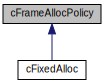
\includegraphics[width=176pt]{d1/d2b/classcFrameAllocPolicy__inherit__graph}
\end{center}
\end{figure}
\subsection*{\-Public \-Member \-Functions}
\begin{DoxyCompactItemize}
\item 
\hypertarget{classcFrameAllocPolicy_a1cae75820fa891b9dd9680c7e72c6903}{void \hyperlink{classcFrameAllocPolicy_a1cae75820fa891b9dd9680c7e72c6903}{set\-Num\-Frames} (int frames)}\label{d3/dd2/classcFrameAllocPolicy_a1cae75820fa891b9dd9680c7e72c6903}

\begin{DoxyCompactList}\small\item\em \-How many frames does the whole system have. \end{DoxyCompactList}\item 
virtual void \hyperlink{classcFrameAllocPolicy_a84e52441bcbb0a571bbcf1a7209cd662}{reg\-Procs} (vector$<$ \hyperlink{structsProc}{s\-Proc} $\ast$ $>$ \&procs)=0
\begin{DoxyCompactList}\small\item\em \-Give the policy module information about processes. \end{DoxyCompactList}\item 
\hypertarget{classcFrameAllocPolicy_a43bd6cfdaa2c03c31dc246c894b03f6c}{virtual pair$<$ bool, uint32\-\_\-t $>$ {\bfseries get\-Frame} (\hyperlink{structsProc}{s\-Proc} $\ast$)=0}\label{d3/dd2/classcFrameAllocPolicy_a43bd6cfdaa2c03c31dc246c894b03f6c}

\item 
virtual void \hyperlink{classcFrameAllocPolicy_a40446e60eefff1fe2a72252af007c877}{return\-Frame} (uint32\-\_\-t frame)=0
\begin{DoxyCompactList}\small\item\em \-System is returning a page. \end{DoxyCompactList}\item 
\hypertarget{classcFrameAllocPolicy_a444e4c60f59041dbd840c18f4fe54a38}{virtual uint32\-\_\-t {\bfseries check\-Open} (bool)=0}\label{d3/dd2/classcFrameAllocPolicy_a444e4c60f59041dbd840c18f4fe54a38}

\item 
\hypertarget{classcFrameAllocPolicy_a3b1e7dc504fdd5f05d99e921b4f696cb}{virtual bool {\bfseries pin} (uint32\-\_\-t frame)=0}\label{d3/dd2/classcFrameAllocPolicy_a3b1e7dc504fdd5f05d99e921b4f696cb}

\item 
\hypertarget{classcFrameAllocPolicy_a1ba7066e5020bbaa48badde38e8208ca}{virtual bool {\bfseries unpin} (uint32\-\_\-t frame)=0}\label{d3/dd2/classcFrameAllocPolicy_a1ba7066e5020bbaa48badde38e8208ca}

\end{DoxyCompactItemize}
\subsection*{\-Private \-Member \-Functions}
\begin{DoxyCompactItemize}
\item 
\hypertarget{classcFrameAllocPolicy_a243b45635bef79761349194f3f994588}{virtual void {\bfseries print\-Frames} ()=0}\label{d3/dd2/classcFrameAllocPolicy_a243b45635bef79761349194f3f994588}

\end{DoxyCompactItemize}
\subsection*{\-Private \-Attributes}
\begin{DoxyCompactItemize}
\item 
\hypertarget{classcFrameAllocPolicy_a0ed4f68c017eadda6155c306cd9f9ae5}{uint32\-\_\-t {\bfseries num\-Frames}}\label{d3/dd2/classcFrameAllocPolicy_a0ed4f68c017eadda6155c306cd9f9ae5}

\end{DoxyCompactItemize}


\subsection{\-Detailed \-Description}
\-The \-V\-M\-M core uses derived classes of this type to decide how many frames to give a process when it is created. 

\subsection{\-Member \-Function \-Documentation}
\hypertarget{classcFrameAllocPolicy_a84e52441bcbb0a571bbcf1a7209cd662}{\index{c\-Frame\-Alloc\-Policy@{c\-Frame\-Alloc\-Policy}!reg\-Procs@{reg\-Procs}}
\index{reg\-Procs@{reg\-Procs}!cFrameAllocPolicy@{c\-Frame\-Alloc\-Policy}}
\subsubsection[{reg\-Procs}]{\setlength{\rightskip}{0pt plus 5cm}virtual void {\bf c\-Frame\-Alloc\-Policy\-::reg\-Procs} (
\begin{DoxyParamCaption}
\item[{vector$<$ {\bf s\-Proc} $\ast$ $>$ \&}]{procs}
\end{DoxyParamCaption}
)\hspace{0.3cm}{\ttfamily  \mbox{[}pure virtual\mbox{]}}}}\label{d3/dd2/classcFrameAllocPolicy_a84e52441bcbb0a571bbcf1a7209cd662}
\-Some frame allocation policies may want information regarding particular processes. \-This is called after construction and it gives the policy a chance to build any necessary datastructures. 

\-Implemented in \hyperlink{classcFixedAlloc_a489395f063815020f36265a52308a3f6}{c\-Fixed\-Alloc}.

\hypertarget{classcFrameAllocPolicy_a40446e60eefff1fe2a72252af007c877}{\index{c\-Frame\-Alloc\-Policy@{c\-Frame\-Alloc\-Policy}!return\-Frame@{return\-Frame}}
\index{return\-Frame@{return\-Frame}!cFrameAllocPolicy@{c\-Frame\-Alloc\-Policy}}
\subsubsection[{return\-Frame}]{\setlength{\rightskip}{0pt plus 5cm}virtual void {\bf c\-Frame\-Alloc\-Policy\-::return\-Frame} (
\begin{DoxyParamCaption}
\item[{uint32\-\_\-t}]{frame}
\end{DoxyParamCaption}
)\hspace{0.3cm}{\ttfamily  \mbox{[}pure virtual\mbox{]}}}}\label{d3/dd2/classcFrameAllocPolicy_a40446e60eefff1fe2a72252af007c877}
\-This could happen on process termination or invocation of the page cleaning daemon. 

\-Implemented in \hyperlink{classcFixedAlloc_a79df79853a015bb750ca682630afcfd8}{c\-Fixed\-Alloc}.



\-Referenced by c\-P\-R\-Fifo\-::clear\-Pages(), c\-P\-R\-Lru\-Approx\-::clear\-Pages(), c\-P\-R\-Lru\-::clear\-Pages(), c\-P\-R\-Fifo\-::return\-Frame(), c\-P\-R\-Lru\-Approx\-::return\-Frame(), and c\-P\-R\-Lru\-::return\-Frame().



\-The documentation for this class was generated from the following file\-:\begin{DoxyCompactItemize}
\item 
include/\-Policy/frame\-Alloc.\-h\end{DoxyCompactItemize}

\hypertarget{classcIDManager}{\section{c\-I\-D\-Manager \-Class \-Reference}
\label{de/dd4/classcIDManager}\index{c\-I\-D\-Manager@{c\-I\-D\-Manager}}
}
\subsection*{\-Public \-Member \-Functions}
\begin{DoxyCompactItemize}
\item 
\hyperlink{classcIDManager_a59021595aaf85ebc151c207a8a04f101}{c\-I\-D\-Manager} (unsigned int start\-I\-D=0)
\item 
unsigned int \hyperlink{classcIDManager_a45420147e785cc219743e9aa2c336501}{get\-I\-D} ()
\item 
void \hyperlink{classcIDManager_a6671d898740f88cf40860b0b9e119b02}{return\-I\-D} (unsigned int id)
\end{DoxyCompactItemize}


\subsection{\-Constructor \& \-Destructor \-Documentation}
\hypertarget{classcIDManager_a59021595aaf85ebc151c207a8a04f101}{\index{c\-I\-D\-Manager@{c\-I\-D\-Manager}!c\-I\-D\-Manager@{c\-I\-D\-Manager}}
\index{c\-I\-D\-Manager@{c\-I\-D\-Manager}!cIDManager@{c\-I\-D\-Manager}}
\subsubsection[{c\-I\-D\-Manager}]{\setlength{\rightskip}{0pt plus 5cm}{\bf c\-I\-D\-Manager\-::c\-I\-D\-Manager} (
\begin{DoxyParamCaption}
\item[{unsigned int}]{start\-I\-D = {\ttfamily 0}}
\end{DoxyParamCaption}
)}}\label{de/dd4/classcIDManager_a59021595aaf85ebc151c207a8a04f101}
\-Creates a new \-I\-D \-Manager object

\-Default start \-I\-D is 0. 

\subsection{\-Member \-Function \-Documentation}
\hypertarget{classcIDManager_a45420147e785cc219743e9aa2c336501}{\index{c\-I\-D\-Manager@{c\-I\-D\-Manager}!get\-I\-D@{get\-I\-D}}
\index{get\-I\-D@{get\-I\-D}!cIDManager@{c\-I\-D\-Manager}}
\subsubsection[{get\-I\-D}]{\setlength{\rightskip}{0pt plus 5cm}unsigned int {\bf c\-I\-D\-Manager\-::get\-I\-D} (
\begin{DoxyParamCaption}
{}
\end{DoxyParamCaption}
)}}\label{de/dd4/classcIDManager_a45420147e785cc219743e9aa2c336501}
\-Reserves a unique \-I\-D

\-Unique is in the sense that no one else is currently using it but it may have been used previously. are distributed in increasing order until \-U\-I\-N\-T\-\_\-\-M\-A\-X is reached. \-After this is reached, \-I\-Ds are given from the queue of returned \-I\-Ds. \-If this queue is empty then an exception is thrown. \hypertarget{classcIDManager_a6671d898740f88cf40860b0b9e119b02}{\index{c\-I\-D\-Manager@{c\-I\-D\-Manager}!return\-I\-D@{return\-I\-D}}
\index{return\-I\-D@{return\-I\-D}!cIDManager@{c\-I\-D\-Manager}}
\subsubsection[{return\-I\-D}]{\setlength{\rightskip}{0pt plus 5cm}void {\bf c\-I\-D\-Manager\-::return\-I\-D} (
\begin{DoxyParamCaption}
\item[{unsigned int}]{id}
\end{DoxyParamCaption}
)}}\label{de/dd4/classcIDManager_a6671d898740f88cf40860b0b9e119b02}
\-Returns an \-I\-D to the manager

\-If the \-I\-D is not equal to the one last given then it is added to a 'free queue'. \-If it is equal to the last one reserved then the \-I\-D counter is simply decremented \-If this last case happens, it causes \hyperlink{classcIDManager_a45420147e785cc219743e9aa2c336501}{c\-I\-D\-Manager\-::get\-I\-D} to stop consuming from the queue and return this newly availabe \-I\-D. 

\-The documentation for this class was generated from the following files\-:\begin{DoxyCompactItemize}
\item 
include/utility/id.\-h\item 
src/utility/id.\-cpp\end{DoxyCompactItemize}

\hypertarget{classcIOControl}{\section{c\-I\-O\-Control \-Class \-Reference}
\label{da/d8f/classcIOControl}\index{c\-I\-O\-Control@{c\-I\-O\-Control}}
}


\-Class representing an \-I/\-O controller.  




{\ttfamily \#include $<$io\-\_\-control.\-h$>$}



\-Collaboration diagram for c\-I\-O\-Control\-:\nopagebreak
\begin{figure}[H]
\begin{center}
\leavevmode
\includegraphics[width=350pt]{d5/db8/classcIOControl__coll__graph}
\end{center}
\end{figure}
\subsection*{\-Public \-Member \-Functions}
\begin{DoxyCompactItemize}
\item 
\hypertarget{classcIOControl_aefe59221a4ffc9df0973e468febf013b}{\hyperlink{classcIOControl_aefe59221a4ffc9df0973e468febf013b}{c\-I\-O\-Control} (int num\-Procs, int $\ast$\-V\-C)}\label{da/d8f/classcIOControl_aefe59221a4ffc9df0973e468febf013b}

\begin{DoxyCompactList}\small\item\em \-Reference virtual counter in core. \end{DoxyCompactList}\item 
queue$<$ uint64\-\_\-t $>$ \& \hyperlink{classcIOControl_a7765e006a0403642713469f9674a1dd3}{get\-Finished\-Queue} ()
\begin{DoxyCompactList}\small\item\em \-Get a reference to the finished queue. \end{DoxyCompactList}\item 
queue$<$ \hyperlink{structsPTE}{s\-P\-T\-E} $\ast$ $>$ \& \hyperlink{classcIOControl_a72bbe2fda30108727eab840aede31b42}{get\-Finished\-P\-T\-E\-Queue} ()
\begin{DoxyCompactList}\small\item\em \-Get a reference to the finished \-P\-T\-E queue. \end{DoxyCompactList}\item 
void \hyperlink{classcIOControl_a820f361e69d99d0da35ebf448643d54a}{tick} ()
\begin{DoxyCompactList}\small\item\em \-Count 1 time unit. \end{DoxyCompactList}\item 
void \hyperlink{classcIOControl_a85b87b93a0b52ba7aa5c3b764f58903d}{tick} (int times)
\begin{DoxyCompactList}\small\item\em \-This executes \-::tick() \-N number of times. \end{DoxyCompactList}\item 
\hyperlink{structsIOContext}{s\-I\-O\-Context} $\ast$ \hyperlink{classcIOControl_a47ac21dd888187a969eec853b7256a83}{schedule\-I\-O} (\hyperlink{structsProc}{s\-Proc} $\ast$proc, uint32\-\_\-t page, e\-I\-O\-Type iotype, \hyperlink{structsIOContext}{s\-I\-O\-Context} $\ast$release=\-N\-U\-L\-L)
\begin{DoxyCompactList}\small\item\em \-Schedule an \-I/\-O event. \end{DoxyCompactList}\end{DoxyCompactItemize}
\subsection*{\-Private \-Member \-Functions}
\begin{DoxyCompactItemize}
\item 
void \hyperlink{classcIOControl_a235b0bd1459463529e1a0b9f07f25ccb}{remove\-Wait} (uint32\-\_\-t)
\begin{DoxyCompactList}\small\item\em \-Remove an \-I/\-O context from waiting. \end{DoxyCompactList}\item 
\hyperlink{structsIOContext}{s\-I\-O\-Context} $\ast$ \hyperlink{classcIOControl_a55df5b64418ea644eb23a6198ff13845}{get\-Context} ()
\begin{DoxyCompactList}\small\item\em \-Get a context struct. \end{DoxyCompactList}\item 
void \hyperlink{classcIOControl_abceaee42b9df46c3fdbd4e26f88e9e88}{return\-Context} (\hyperlink{structsIOContext}{s\-I\-O\-Context} $\ast$ctx)
\begin{DoxyCompactList}\small\item\em \-Return a context struct for future use. \end{DoxyCompactList}\item 
void \hyperlink{classcIOControl_ac0839c4c60b08a2cfa425d3c90d584f3}{dump\-I\-O\-Error} (\hyperlink{structsProc}{s\-Proc} $\ast$)
\begin{DoxyCompactList}\small\item\em \-Generate and throw \-I\-O \-Error. \end{DoxyCompactList}\end{DoxyCompactItemize}
\subsection*{\-Private \-Attributes}
\begin{DoxyCompactItemize}
\item 
\hypertarget{classcIOControl_a4b9aa88be2dc67cf9ed33051dba6eebb}{int {\bfseries io\-\_\-req\-\_\-time}}\label{da/d8f/classcIOControl_a4b9aa88be2dc67cf9ed33051dba6eebb}

\item 
\hypertarget{classcIOControl_aacf61a8d660e60a7e444e32474b7875a}{int {\bfseries io\-\_\-time}}\label{da/d8f/classcIOControl_aacf61a8d660e60a7e444e32474b7875a}

\item 
vector$<$ queue$<$ \hyperlink{structsIOContext}{s\-I\-O\-Context} $\ast$ $>$ $>$ \hyperlink{classcIOControl_a51a2c3ce8bf36b9302d835afb204c821}{io\-\_\-out}
\begin{DoxyCompactList}\small\item\em \-What is being paged out? \end{DoxyCompactList}\item 
\hypertarget{classcIOControl_abb546a7c4d622af5e4a95a5742c33b10}{vector$<$ queue$<$ \hyperlink{structsIOContext}{s\-I\-O\-Context} $\ast$ $>$\*
 $>$\-::iterator {\bfseries out\-\_\-iter}}\label{da/d8f/classcIOControl_abb546a7c4d622af5e4a95a5742c33b10}

\item 
queue$<$ \hyperlink{structsIOContext}{s\-I\-O\-Context} $\ast$ $>$ \hyperlink{classcIOControl_a6918230a2e9f6e1e5fdade78da2d835b}{io\-\_\-in}
\begin{DoxyCompactList}\small\item\em \-What is the next page in? \end{DoxyCompactList}\item 
\hypertarget{classcIOControl_a8e33089e107631ba9cc042d72939d913}{vector$<$ \hyperlink{structsIOContext}{s\-I\-O\-Context} $\ast$ $>$ \hyperlink{classcIOControl_a8e33089e107631ba9cc042d72939d913}{io\-\_\-in\-\_\-wait}}\label{da/d8f/classcIOControl_a8e33089e107631ba9cc042d72939d913}

\begin{DoxyCompactList}\small\item\em \-I/\-O in requests waiting for an io\-\_\-out to finish. \end{DoxyCompactList}\item 
\hypertarget{classcIOControl_a3bfc00997effdb1cd33c02bba4a12337}{vector$<$ \hyperlink{structsIOContext}{s\-I\-O\-Context} $\ast$ $>$\-::iterator {\bfseries in\-\_\-wait\-\_\-iter}}\label{da/d8f/classcIOControl_a3bfc00997effdb1cd33c02bba4a12337}

\item 
queue$<$ \hyperlink{structsIOContext}{s\-I\-O\-Context} $\ast$ $>$ \hyperlink{classcIOControl_a52a5d360ffc2f48ee75cac0c801642fd}{context\-\_\-cache}
\begin{DoxyCompactList}\small\item\em \-Cache of previously allocated contexts. \end{DoxyCompactList}\item 
queue$<$ uint64\-\_\-t $>$ \hyperlink{classcIOControl_a193b1bb6dd1b919dbf7de9ce02bf56ad}{finished}
\begin{DoxyCompactList}\small\item\em \-Queue that holds process ids that have completed and \-I/\-O. \end{DoxyCompactList}\item 
\hypertarget{classcIOControl_a57a24ad208c4a16e38935c000383a23e}{queue$<$ \hyperlink{structsPTE}{s\-P\-T\-E} $\ast$ $>$ \hyperlink{classcIOControl_a57a24ad208c4a16e38935c000383a23e}{finished\-P\-T\-E}}\label{da/d8f/classcIOControl_a57a24ad208c4a16e38935c000383a23e}

\begin{DoxyCompactList}\small\item\em \-Holds the \-P\-T\-E of finished \-I/\-O in's. \end{DoxyCompactList}\item 
\hypertarget{classcIOControl_aad4dedae2daa73a6d84bba3af1f1dc45}{int $\ast$ {\bfseries \-V\-C}}\label{da/d8f/classcIOControl_aad4dedae2daa73a6d84bba3af1f1dc45}

\end{DoxyCompactItemize}


\subsection{\-Member \-Function \-Documentation}
\hypertarget{classcIOControl_ac0839c4c60b08a2cfa425d3c90d584f3}{\index{c\-I\-O\-Control@{c\-I\-O\-Control}!dump\-I\-O\-Error@{dump\-I\-O\-Error}}
\index{dump\-I\-O\-Error@{dump\-I\-O\-Error}!cIOControl@{c\-I\-O\-Control}}
\subsubsection[{dump\-I\-O\-Error}]{\setlength{\rightskip}{0pt plus 5cm}{\bf c\-I\-O\-Control\-::dump\-I\-O\-Error} (
\begin{DoxyParamCaption}
\item[{{\bf s\-Proc} $\ast$}]{proc}
\end{DoxyParamCaption}
)\hspace{0.3cm}{\ttfamily  \mbox{[}private\mbox{]}}}}\label{da/d8f/classcIOControl_ac0839c4c60b08a2cfa425d3c90d584f3}
\-This does the work of generating an \-I\-O excetion.\-It was originally intended to work broadly for many different scenarios but the necessity was not there. \-It works but it produces a fairly generic error. 

\-Referenced by schedule\-I\-O().

\hypertarget{classcIOControl_a55df5b64418ea644eb23a6198ff13845}{\index{c\-I\-O\-Control@{c\-I\-O\-Control}!get\-Context@{get\-Context}}
\index{get\-Context@{get\-Context}!cIOControl@{c\-I\-O\-Control}}
\subsubsection[{get\-Context}]{\setlength{\rightskip}{0pt plus 5cm}{\bf c\-I\-O\-Control\-::get\-Context} (
\begin{DoxyParamCaption}
{}
\end{DoxyParamCaption}
)\hspace{0.3cm}{\ttfamily  \mbox{[}private\mbox{]}}}}\label{da/d8f/classcIOControl_a55df5b64418ea644eb23a6198ff13845}
\-If there is a context struct cached from previous use then it is returned. \-Otherwise a new one is allocated. 

\-Referenced by schedule\-I\-O().

\hypertarget{classcIOControl_a72bbe2fda30108727eab840aede31b42}{\index{c\-I\-O\-Control@{c\-I\-O\-Control}!get\-Finished\-P\-T\-E\-Queue@{get\-Finished\-P\-T\-E\-Queue}}
\index{get\-Finished\-P\-T\-E\-Queue@{get\-Finished\-P\-T\-E\-Queue}!cIOControl@{c\-I\-O\-Control}}
\subsubsection[{get\-Finished\-P\-T\-E\-Queue}]{\setlength{\rightskip}{0pt plus 5cm}{\bf c\-I\-O\-Control\-::get\-Finished\-P\-T\-E\-Queue} (
\begin{DoxyParamCaption}
{}
\end{DoxyParamCaption}
)\hspace{0.3cm}{\ttfamily  \mbox{[}inline\mbox{]}}}}\label{da/d8f/classcIOControl_a72bbe2fda30108727eab840aede31b42}
\-This is called by the core to get a reference to this specific queue to be used in processing finished \-I/\-O. \-The purpose for this queue was that the \-V\-M\-M core needed the frame of the completed \-I/\-O so it could be unpinned. \-Given the \-P\-T\-E in this queue it makes page data in the finished queue redundant. 

\-Referenced by c\-V\-M\-M\-::start().

\hypertarget{classcIOControl_a7765e006a0403642713469f9674a1dd3}{\index{c\-I\-O\-Control@{c\-I\-O\-Control}!get\-Finished\-Queue@{get\-Finished\-Queue}}
\index{get\-Finished\-Queue@{get\-Finished\-Queue}!cIOControl@{c\-I\-O\-Control}}
\subsubsection[{get\-Finished\-Queue}]{\setlength{\rightskip}{0pt plus 5cm}{\bf c\-I\-O\-Control\-::get\-Finished\-Queue} (
\begin{DoxyParamCaption}
{}
\end{DoxyParamCaption}
)\hspace{0.3cm}{\ttfamily  \mbox{[}inline\mbox{]}}}}\label{da/d8f/classcIOControl_a7765e006a0403642713469f9674a1dd3}
\-This is called by the core to get a refernce to this specific queue so it can be used in processing finished \-I/\-O. \-This queue hold 64-\/bit integers representing the pid and page of for the completed \-I/\-O. 

\-Referenced by c\-V\-M\-M\-::start().

\hypertarget{classcIOControl_a235b0bd1459463529e1a0b9f07f25ccb}{\index{c\-I\-O\-Control@{c\-I\-O\-Control}!remove\-Wait@{remove\-Wait}}
\index{remove\-Wait@{remove\-Wait}!cIOControl@{c\-I\-O\-Control}}
\subsubsection[{remove\-Wait}]{\setlength{\rightskip}{0pt plus 5cm}{\bf c\-I\-O\-Control\-::remove\-Wait} (
\begin{DoxyParamCaption}
\item[{uint32\-\_\-t}]{pid}
\end{DoxyParamCaption}
)\hspace{0.3cm}{\ttfamily  \mbox{[}private\mbox{]}}}}\label{da/d8f/classcIOControl_a235b0bd1459463529e1a0b9f07f25ccb}
\-When an \-I/\-O out completes, if its release context property is not null then the controller will try to release the specified context from the waiting vector. 

\-Referenced by tick().

\hypertarget{classcIOControl_abceaee42b9df46c3fdbd4e26f88e9e88}{\index{c\-I\-O\-Control@{c\-I\-O\-Control}!return\-Context@{return\-Context}}
\index{return\-Context@{return\-Context}!cIOControl@{c\-I\-O\-Control}}
\subsubsection[{return\-Context}]{\setlength{\rightskip}{0pt plus 5cm}{\bf c\-I\-O\-Control\-::return\-Context} (
\begin{DoxyParamCaption}
\item[{{\bf s\-I\-O\-Context} $\ast$}]{ctx}
\end{DoxyParamCaption}
)\hspace{0.3cm}{\ttfamily  \mbox{[}private\mbox{]}}}}\label{da/d8f/classcIOControl_abceaee42b9df46c3fdbd4e26f88e9e88}
\-The struct is not deallocated. \-It is put into a cache queue. 

\-Referenced by tick().

\hypertarget{classcIOControl_a47ac21dd888187a969eec853b7256a83}{\index{c\-I\-O\-Control@{c\-I\-O\-Control}!schedule\-I\-O@{schedule\-I\-O}}
\index{schedule\-I\-O@{schedule\-I\-O}!cIOControl@{c\-I\-O\-Control}}
\subsubsection[{schedule\-I\-O}]{\setlength{\rightskip}{0pt plus 5cm}{\bf c\-I\-O\-Control\-::schedule\-I\-O} (
\begin{DoxyParamCaption}
\item[{{\bf s\-Proc} $\ast$}]{proc, }
\item[{uint32\-\_\-t}]{page, }
\item[{e\-I\-O\-Type}]{iotype, }
\item[{{\bf s\-I\-O\-Context} $\ast$}]{release = {\ttfamily \-N\-U\-L\-L}}
\end{DoxyParamCaption}
)}}\label{da/d8f/classcIOControl_a47ac21dd888187a969eec853b7256a83}
\-Schedule \-I/\-O.

\-This is used to schedule some \-I/\-O. \-The type is specified by the e\-I\-O\-Type parameter. \-If the type is e\-I\-O\-Type\-::\-I\-O\-\_\-\-I\-N\-\_\-\-W\-A\-I\-T it will be put in a vector (indexed by pid) waiting to be released. \-If the type is e\-I\-O\-Type\-::\-I\-O\-\_\-\-O\-U\-T and the s\-I\-O\-Context$\ast$ != \-N\-U\-L\-L then after the \-I/\-O completes it will relese the \-I/\-O pointed to by this context. 

\-Referenced by c\-V\-M\-M\-::page\-In(), and c\-V\-M\-M\-::page\-Out().

\hypertarget{classcIOControl_a820f361e69d99d0da35ebf448643d54a}{\index{c\-I\-O\-Control@{c\-I\-O\-Control}!tick@{tick}}
\index{tick@{tick}!cIOControl@{c\-I\-O\-Control}}
\subsubsection[{tick}]{\setlength{\rightskip}{0pt plus 5cm}{\bf c\-I\-O\-Control\-::tick} (
\begin{DoxyParamCaption}
{}
\end{DoxyParamCaption}
)}}\label{da/d8f/classcIOControl_a820f361e69d99d0da35ebf448643d54a}
\-Thiscounts 1 virtual time unite and modifies the remaining time on pending \-I/\-O correspondingly. 

\-Referenced by schedule\-I\-O(), c\-V\-M\-M\-::start(), tick(), and c\-V\-M\-M\-::tick\-Controller().

\hypertarget{classcIOControl_a85b87b93a0b52ba7aa5c3b764f58903d}{\index{c\-I\-O\-Control@{c\-I\-O\-Control}!tick@{tick}}
\index{tick@{tick}!cIOControl@{c\-I\-O\-Control}}
\subsubsection[{tick}]{\setlength{\rightskip}{0pt plus 5cm}{\bf c\-I\-O\-Control\-::tick} (
\begin{DoxyParamCaption}
\item[{int}]{times}
\end{DoxyParamCaption}
)}}\label{da/d8f/classcIOControl_a85b87b93a0b52ba7aa5c3b764f58903d}
\-This is useful in recording virtual time with events that take chunks of time such as the context switching of a process.


\begin{DoxyParams}{\-Parameters}
{\em int} & \-Number of ticks to execute. \\
\hline
\end{DoxyParams}


\subsection{\-Member \-Data \-Documentation}
\hypertarget{classcIOControl_a52a5d360ffc2f48ee75cac0c801642fd}{\index{c\-I\-O\-Control@{c\-I\-O\-Control}!context\-\_\-cache@{context\-\_\-cache}}
\index{context\-\_\-cache@{context\-\_\-cache}!cIOControl@{c\-I\-O\-Control}}
\subsubsection[{context\-\_\-cache}]{\setlength{\rightskip}{0pt plus 5cm}queue$<${\bf s\-I\-O\-Context}$\ast$$>$ {\bf c\-I\-O\-Control\-::context\-\_\-cache}\hspace{0.3cm}{\ttfamily  \mbox{[}private\mbox{]}}}}\label{da/d8f/classcIOControl_a52a5d360ffc2f48ee75cac0c801642fd}
\-This is simply a performance boost to avoid constantly allocating/deallocating context structs. 

\-Referenced by get\-Context(), and return\-Context().

\hypertarget{classcIOControl_a193b1bb6dd1b919dbf7de9ce02bf56ad}{\index{c\-I\-O\-Control@{c\-I\-O\-Control}!finished@{finished}}
\index{finished@{finished}!cIOControl@{c\-I\-O\-Control}}
\subsubsection[{finished}]{\setlength{\rightskip}{0pt plus 5cm}queue$<$uint64\-\_\-t$>$ {\bf c\-I\-O\-Control\-::finished}\hspace{0.3cm}{\ttfamily  \mbox{[}private\mbox{]}}}}\label{da/d8f/classcIOControl_a193b1bb6dd1b919dbf7de9ce02bf56ad}
\-This is specifically used for completed page ins. \-After calling tick, any completed processes are placed in here and the \-V\-M\-M core can read it and unblock.

\-I made it a 64-\/bit data type so that \-I didn't need to mess with allocating and managing some other structure. \-The first 32-\/bits represent the pid of the process whose \-I/\-O completed. \-The last 32-\/bits is the page that was brought in for the process. \-From this the core can get the frame and unpin it. 

\-Referenced by tick().

\hypertarget{classcIOControl_a6918230a2e9f6e1e5fdade78da2d835b}{\index{c\-I\-O\-Control@{c\-I\-O\-Control}!io\-\_\-in@{io\-\_\-in}}
\index{io\-\_\-in@{io\-\_\-in}!cIOControl@{c\-I\-O\-Control}}
\subsubsection[{io\-\_\-in}]{\setlength{\rightskip}{0pt plus 5cm}queue$<${\bf s\-I\-O\-Context}$\ast$$>$ {\bf c\-I\-O\-Control\-::io\-\_\-in}\hspace{0.3cm}{\ttfamily  \mbox{[}private\mbox{]}}}}\label{da/d8f/classcIOControl_a6918230a2e9f6e1e5fdade78da2d835b}
\-This keeps track of the next page to complete its \-I/\-O. 

\-Referenced by remove\-Wait(), schedule\-I\-O(), and tick().

\hypertarget{classcIOControl_a51a2c3ce8bf36b9302d835afb204c821}{\index{c\-I\-O\-Control@{c\-I\-O\-Control}!io\-\_\-out@{io\-\_\-out}}
\index{io\-\_\-out@{io\-\_\-out}!cIOControl@{c\-I\-O\-Control}}
\subsubsection[{io\-\_\-out}]{\setlength{\rightskip}{0pt plus 5cm}vector$<$queue$<${\bf s\-I\-O\-Context}$\ast$$>$ $>$ {\bf c\-I\-O\-Control\-::io\-\_\-out}\hspace{0.3cm}{\ttfamily  \mbox{[}private\mbox{]}}}}\label{da/d8f/classcIOControl_a51a2c3ce8bf36b9302d835afb204c821}
\-This vector is indexed by pid and it holds a queue of the pages of the respective process which are being paged out. \-This is so that in the case that a process has a page spilled by some other process' page fault or the cleaning daemon, it is prevented from recovering the page until it is successfully written out. 

\-Referenced by c\-I\-O\-Control(), schedule\-I\-O(), and tick().



\-The documentation for this class was generated from the following files\-:\begin{DoxyCompactItemize}
\item 
include/io\-\_\-control.\-h\item 
src/io\-\_\-control.\-cpp\end{DoxyCompactItemize}

\hypertarget{classcIOExc}{\section{c\-I\-O\-Exc \-Class \-Reference}
\label{d3/dbc/classcIOExc}\index{c\-I\-O\-Exc@{c\-I\-O\-Exc}}
}


\-Class handling exceptions in the \-I/\-O system.  




{\ttfamily \#include $<$exceptions.\-h$>$}



\-Inheritance diagram for c\-I\-O\-Exc\-:\nopagebreak
\begin{figure}[H]
\begin{center}
\leavevmode
\includegraphics[width=144pt]{de/d6d/classcIOExc__inherit__graph}
\end{center}
\end{figure}


\-Collaboration diagram for c\-I\-O\-Exc\-:\nopagebreak
\begin{figure}[H]
\begin{center}
\leavevmode
\includegraphics[width=144pt]{df/db5/classcIOExc__coll__graph}
\end{center}
\end{figure}
\subsection*{\-Public \-Member \-Functions}
\begin{DoxyCompactItemize}
\item 
\hypertarget{classcIOExc_a8659256c4ce821f1b243d32c2164ad08}{void {\bfseries set\-Trace} (const string \&trace)}\label{d3/dbc/classcIOExc_a8659256c4ce821f1b243d32c2164ad08}

\item 
\hypertarget{classcIOExc_abf33ecff4f124c536a66fab8740d4e72}{string \& {\bfseries get\-Trace} ()}\label{d3/dbc/classcIOExc_abf33ecff4f124c536a66fab8740d4e72}

\end{DoxyCompactItemize}
\subsection*{\-Private \-Attributes}
\begin{DoxyCompactItemize}
\item 
\hypertarget{classcIOExc_ad01c3157522f9c4bbb6caf7a551fc8de}{string {\bfseries \-I\-O\-\_\-\-Data\-\_\-\-Trace}}\label{d3/dbc/classcIOExc_ad01c3157522f9c4bbb6caf7a551fc8de}

\end{DoxyCompactItemize}


\-The documentation for this class was generated from the following file\-:\begin{DoxyCompactItemize}
\item 
include/\hyperlink{exceptions_8h}{exceptions.\-h}\end{DoxyCompactItemize}

\hypertarget{classcMMU}{\section{c\-M\-M\-U \-Class \-Reference}
\label{df/deb/classcMMU}\index{c\-M\-M\-U@{c\-M\-M\-U}}
}


\-Collaboration diagram for c\-M\-M\-U\-:\nopagebreak
\begin{figure}[H]
\begin{center}
\leavevmode
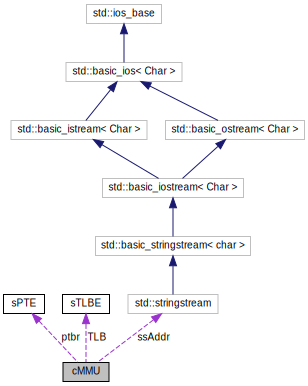
\includegraphics[width=350pt]{dc/d5d/classcMMU__coll__graph}
\end{center}
\end{figure}
\subsection*{\-Public \-Member \-Functions}
\begin{DoxyCompactItemize}
\item 
\hypertarget{classcMMU_a07912c15eb7a743c0736f3b4e9616860}{void {\bfseries set\-P\-T\-B\-R} (\hyperlink{structsPTE}{s\-P\-T\-E} $\ast$\-\_\-ptbr)}\label{df/deb/classcMMU_a07912c15eb7a743c0736f3b4e9616860}

\item 
\hypertarget{classcMMU_af6b2683d1514d5587d8a48c2dc025f5e}{void {\bfseries add\-V\-C} (int $\ast$\-V\-C)}\label{df/deb/classcMMU_af6b2683d1514d5587d8a48c2dc025f5e}

\item 
\hypertarget{classcMMU_a551b571684c7203e0993d3270316e75e}{void {\bfseries flush\-T\-L\-B} (bool sync=true)}\label{df/deb/classcMMU_a551b571684c7203e0993d3270316e75e}

\item 
\hypertarget{classcMMU_ab36461a16e1a4a073a025bd91b8ba519}{void {\bfseries sync\-T\-L\-B} ()}\label{df/deb/classcMMU_ab36461a16e1a4a073a025bd91b8ba519}

\item 
\hypertarget{classcMMU_a85181f4d23360667aec58e6822c6889b}{e\-M\-M\-Ustate {\bfseries check\-Status} ()}\label{df/deb/classcMMU_a85181f4d23360667aec58e6822c6889b}

\item 
\hypertarget{classcMMU_a755d689d330c8283f1d6183c1e5cbcc1}{uint32\-\_\-t {\bfseries get\-Fault\-Page} ()}\label{df/deb/classcMMU_a755d689d330c8283f1d6183c1e5cbcc1}

\item 
uint32\-\_\-t \hyperlink{classcMMU_a8f67a55d3444b1164999ef64253eb37e}{get\-Addr} (string \&s\-V\-A, bool is\-Write)
\begin{DoxyCompactList}\small\item\em \-Translate virtual to physical address. \end{DoxyCompactList}\end{DoxyCompactItemize}
\subsection*{\-Private \-Member \-Functions}
\begin{DoxyCompactItemize}
\item 
\hypertarget{classcMMU_a9cc1d030c6180c32aa9e6308a6a7c66c}{void {\bfseries add\-T\-L\-B} (uint32\-\_\-t, uint32\-\_\-t, bool)}\label{df/deb/classcMMU_a9cc1d030c6180c32aa9e6308a6a7c66c}

\end{DoxyCompactItemize}
\subsection*{\-Private \-Attributes}
\begin{DoxyCompactItemize}
\item 
\hypertarget{classcMMU_a0d648c0b2700336ccd048d338e3c0f40}{\hyperlink{structsTLBE}{s\-T\-L\-B\-E} $\ast$ {\bfseries \-T\-L\-B}}\label{df/deb/classcMMU_a0d648c0b2700336ccd048d338e3c0f40}

\item 
\hypertarget{classcMMU_a33bae6bddbaa164c3c8bec3369dac99e}{uint16\-\_\-t {\bfseries tlb\-Size}}\label{df/deb/classcMMU_a33bae6bddbaa164c3c8bec3369dac99e}

\item 
\hypertarget{classcMMU_a518605a6810c2db0e4c3c6118d68eecd}{uint32\-\_\-t {\bfseries page\-Size}}\label{df/deb/classcMMU_a518605a6810c2db0e4c3c6118d68eecd}

\item 
\hypertarget{classcMMU_a00cef287ae02c5007a3462d833b2aaaa}{uint32\-\_\-t {\bfseries off\-\_\-bits}}\label{df/deb/classcMMU_a00cef287ae02c5007a3462d833b2aaaa}

\item 
\hypertarget{classcMMU_ac747da0e08fa4988c1f1d6c0b89ec304}{bool {\bfseries hex\-Addr}}\label{df/deb/classcMMU_ac747da0e08fa4988c1f1d6c0b89ec304}

\item 
\hypertarget{classcMMU_a3a3f41d64f9d10bcd75d04553c7d2fbb}{stringstream {\bfseries ss\-Addr}}\label{df/deb/classcMMU_a3a3f41d64f9d10bcd75d04553c7d2fbb}

\item 
uint32\-\_\-t \hyperlink{classcMMU_a90cbcd50347e8b9030f66bce2fc52e2a}{replace\-Index}
\begin{DoxyCompactList}\small\item\em \-For replacing old tlb entries we are simply treating it as a ring buffer. \end{DoxyCompactList}\item 
\hypertarget{classcMMU_a32b0fcd59b1afd0a73170cc6f10b4e8e}{int $\ast$ {\bfseries \-V\-C}}\label{df/deb/classcMMU_a32b0fcd59b1afd0a73170cc6f10b4e8e}

\item 
\hypertarget{classcMMU_ac2cb598634fc88375313eac3d9ec9348}{\hyperlink{structsPTE}{s\-P\-T\-E} $\ast$ {\bfseries ptbr}}\label{df/deb/classcMMU_ac2cb598634fc88375313eac3d9ec9348}

\item 
\hypertarget{classcMMU_ad127c2a2928e67b8a201319e00215d86}{int {\bfseries tlb\-\_\-hits}}\label{df/deb/classcMMU_ad127c2a2928e67b8a201319e00215d86}

\item 
\hypertarget{classcMMU_af9b299f41ac146cca9982cd2768b3945}{int {\bfseries tlb\-\_\-misses}}\label{df/deb/classcMMU_af9b299f41ac146cca9982cd2768b3945}

\item 
\hypertarget{classcMMU_a593631c8752611c58c8ddd5a82f24d9e}{e\-M\-M\-Ustate {\bfseries mmu\-\_\-status}}\label{df/deb/classcMMU_a593631c8752611c58c8ddd5a82f24d9e}

\item 
\hypertarget{classcMMU_a719786f4271afae04e95286bf9bcdd81}{uint32\-\_\-t {\bfseries fault\-Page}}\label{df/deb/classcMMU_a719786f4271afae04e95286bf9bcdd81}

\end{DoxyCompactItemize}


\subsection{\-Member \-Function \-Documentation}
\hypertarget{classcMMU_a8f67a55d3444b1164999ef64253eb37e}{\index{c\-M\-M\-U@{c\-M\-M\-U}!get\-Addr@{get\-Addr}}
\index{get\-Addr@{get\-Addr}!cMMU@{c\-M\-M\-U}}
\subsubsection[{get\-Addr}]{\setlength{\rightskip}{0pt plus 5cm}uint32\-\_\-t {\bf c\-M\-M\-U\-::get\-Addr} (
\begin{DoxyParamCaption}
\item[{string \&}]{s\-V\-A, }
\item[{bool}]{is\-Write}
\end{DoxyParamCaption}
)}}\label{df/deb/classcMMU_a8f67a55d3444b1164999ef64253eb37e}
\-This method checks the tlb and page table simultaneously and returns the appropriate address. \-Whoever receives this should first check the mmu status to make sure it is valid.


\begin{DoxyParams}{\-Parameters}
{\em bool} & write \-If set, the mmu will mark this page as dirty. \\
\hline
\end{DoxyParams}


\-Referenced by c\-C\-P\-U\-::run().



\subsection{\-Member \-Data \-Documentation}
\hypertarget{classcMMU_a90cbcd50347e8b9030f66bce2fc52e2a}{\index{c\-M\-M\-U@{c\-M\-M\-U}!replace\-Index@{replace\-Index}}
\index{replace\-Index@{replace\-Index}!cMMU@{c\-M\-M\-U}}
\subsubsection[{replace\-Index}]{\setlength{\rightskip}{0pt plus 5cm}uint32\-\_\-t {\bf c\-M\-M\-U\-::replace\-Index}\hspace{0.3cm}{\ttfamily  \mbox{[}private\mbox{]}}}}\label{df/deb/classcMMU_a90cbcd50347e8b9030f66bce2fc52e2a}
\-This is the index where new entries are being placed 

\-The documentation for this class was generated from the following files\-:\begin{DoxyCompactItemize}
\item 
include/mmu.\-h\item 
src/mmu.\-cpp\end{DoxyCompactItemize}

\hypertarget{classcPRExc}{\section{c\-P\-R\-Exc \-Class \-Reference}
\label{d5/d34/classcPRExc}\index{c\-P\-R\-Exc@{c\-P\-R\-Exc}}
}


\-Exception specific to the \-P\-R module.  




{\ttfamily \#include $<$exceptions.\-h$>$}



\-Inheritance diagram for c\-P\-R\-Exc\-:\nopagebreak
\begin{figure}[H]
\begin{center}
\leavevmode
\includegraphics[width=144pt]{d0/da7/classcPRExc__inherit__graph}
\end{center}
\end{figure}


\-Collaboration diagram for c\-P\-R\-Exc\-:\nopagebreak
\begin{figure}[H]
\begin{center}
\leavevmode
\includegraphics[width=144pt]{de/d3b/classcPRExc__coll__graph}
\end{center}
\end{figure}
\subsection*{\-Public \-Member \-Functions}
\begin{DoxyCompactItemize}
\item 
\hypertarget{classcPRExc_a24b4994c84da2efc6fa6652d15809e14}{void {\bfseries set\-Name} (const string \&\-\_\-name)}\label{d5/d34/classcPRExc_a24b4994c84da2efc6fa6652d15809e14}

\end{DoxyCompactItemize}
\subsection*{\-Private \-Attributes}
\begin{DoxyCompactItemize}
\item 
\hypertarget{classcPRExc_a153e6dec3f6fdf2cd4565ecc83a20599}{string {\bfseries name}}\label{d5/d34/classcPRExc_a153e6dec3f6fdf2cd4565ecc83a20599}

\end{DoxyCompactItemize}


\-The documentation for this class was generated from the following file\-:\begin{DoxyCompactItemize}
\item 
include/\hyperlink{exceptions_8h}{exceptions.\-h}\end{DoxyCompactItemize}

\hypertarget{classcPRFifo}{\section{c\-P\-R\-Fifo \-Class \-Reference}
\label{db/d3a/classcPRFifo}\index{c\-P\-R\-Fifo@{c\-P\-R\-Fifo}}
}


\-Inheritance diagram for c\-P\-R\-Fifo\-:\nopagebreak
\begin{figure}[H]
\begin{center}
\leavevmode
\includegraphics[width=142pt]{d6/d49/classcPRFifo__inherit__graph}
\end{center}
\end{figure}


\-Collaboration diagram for c\-P\-R\-Fifo\-:\nopagebreak
\begin{figure}[H]
\begin{center}
\leavevmode
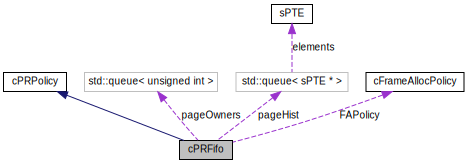
\includegraphics[width=350pt]{d9/d21/classcPRFifo__coll__graph}
\end{center}
\end{figure}
\subsection*{\-Public \-Member \-Functions}
\begin{DoxyCompactItemize}
\item 
\hypertarget{classcPRFifo_a87ea4d98314c4418060e57982414a39f}{{\bfseries c\-P\-R\-Fifo} (\hyperlink{classcFrameAllocPolicy}{c\-Frame\-Alloc\-Policy} \&\-\_\-\-F\-A\-Policy)}\label{db/d3a/classcPRFifo_a87ea4d98314c4418060e57982414a39f}

\item 
const char $\ast$ \hyperlink{classcPRFifo_aa3b9269589ccebd364d07ef69015bad6}{name} ()
\begin{DoxyCompactList}\small\item\em \-Name of \-P\-R module. \end{DoxyCompactList}\item 
\hyperlink{pageReplace_8h_af4bc4c41a44c2bd80e8cbf1aae370217}{e\-P\-R\-Status} \hyperlink{classcPRFifo_a8121128a2dac3c8194c044e81fa0e5fc}{resolve\-Page\-Fault} (\hyperlink{structsProc}{s\-Proc} $\ast$proc, uint32\-\_\-t page)
\begin{DoxyCompactList}\small\item\em \-Get a page frame for this process. \end{DoxyCompactList}\item 
void \hyperlink{classcPRFifo_aadb8319e6e539280e0f56c0e6b40c581}{finished\-Quanta} (\hyperlink{structsProc}{s\-Proc} $\ast$proc)
\begin{DoxyCompactList}\small\item\em \-This is called after an execution quanta finishes. \end{DoxyCompactList}\item 
void \hyperlink{classcPRFifo_a158824c0cf38fa23a14f7148431bc34d}{finished\-I\-O} (\hyperlink{structsProc}{s\-Proc} $\ast$proc, \hyperlink{structsPTE}{s\-P\-T\-E} $\ast$page)
\begin{DoxyCompactList}\small\item\em \-This is called after an \-I/\-O (input) completes. \end{DoxyCompactList}\item 
bool \hyperlink{classcPRFifo_ab2bca492cfd0a628df492781ecd726ff}{clear\-Pages} (int num\-Pages)
\begin{DoxyCompactList}\small\item\em \-Remove this many pages from memory. \end{DoxyCompactList}\item 
\hypertarget{classcPRFifo_ac2bfc42038801005f9dbfed30d583bca}{void \hyperlink{classcPRFifo_ac2bfc42038801005f9dbfed30d583bca}{unpin\-Frame} (uint32\-\_\-t frame)}\label{db/d3a/classcPRFifo_ac2bfc42038801005f9dbfed30d583bca}

\begin{DoxyCompactList}\small\item\em \-This is typically called after \-::finished\-I\-O so that the \-P\-R module unpins the frame in the frame allocation module. \end{DoxyCompactList}\item 
void \hyperlink{classcPRFifo_a8155953bcbd7a0799d07a8228dc0e80c}{return\-Frame} (uint32\-\_\-t frame)
\begin{DoxyCompactList}\small\item\em \-Return a frame to the system. \end{DoxyCompactList}\end{DoxyCompactItemize}
\subsection*{\-Private \-Attributes}
\begin{DoxyCompactItemize}
\item 
\hypertarget{classcPRFifo_a55cd40966135c67531087a943d69cd8a}{queue$<$ \hyperlink{structsPTE}{s\-P\-T\-E} $\ast$ $>$ {\bfseries page\-Hist}}\label{db/d3a/classcPRFifo_a55cd40966135c67531087a943d69cd8a}

\item 
\hypertarget{classcPRFifo_ac2eb1d98dce1f4d65fb50de514bff2c6}{queue$<$ unsigned int $>$ {\bfseries page\-Owners}}\label{db/d3a/classcPRFifo_ac2eb1d98dce1f4d65fb50de514bff2c6}

\item 
\hypertarget{classcPRFifo_af559318a9aec1a9bb80316fe75c95ebf}{\hyperlink{classcFrameAllocPolicy}{c\-Frame\-Alloc\-Policy} \& {\bfseries \-F\-A\-Policy}}\label{db/d3a/classcPRFifo_af559318a9aec1a9bb80316fe75c95ebf}

\item 
\hypertarget{classcPRFifo_ae007331b8af8dc84c4833846f7ca6dde}{uint32\-\_\-t {\bfseries \-P\-T\-Size}}\label{db/d3a/classcPRFifo_ae007331b8af8dc84c4833846f7ca6dde}

\end{DoxyCompactItemize}


\subsection{\-Member \-Function \-Documentation}
\hypertarget{classcPRFifo_ab2bca492cfd0a628df492781ecd726ff}{\index{c\-P\-R\-Fifo@{c\-P\-R\-Fifo}!clear\-Pages@{clear\-Pages}}
\index{clear\-Pages@{clear\-Pages}!cPRFifo@{c\-P\-R\-Fifo}}
\subsubsection[{clear\-Pages}]{\setlength{\rightskip}{0pt plus 5cm}bool {\bf c\-P\-R\-Fifo\-::clear\-Pages} (
\begin{DoxyParamCaption}
\item[{int}]{num\-Pages}
\end{DoxyParamCaption}
)\hspace{0.3cm}{\ttfamily  \mbox{[}virtual\mbox{]}}}}\label{db/d3a/classcPRFifo_ab2bca492cfd0a628df492781ecd726ff}
\-If the cleaning daemon decides that pages need to be cleaned it will determine how many from its policy and call the \-P\-R module to clean that many. \-This method keeps the \-P\-R policy separate from the decision on how many pages to clean and when.


\begin{DoxyParams}{\-Parameters}
{\em int} & \-Number of pages to clear. \\
\hline
\end{DoxyParams}


\-Implements \hyperlink{classcPRPolicy_a7a2b6d5761963a69d20794579d39530f}{c\-P\-R\-Policy}.

\hypertarget{classcPRFifo_a158824c0cf38fa23a14f7148431bc34d}{\index{c\-P\-R\-Fifo@{c\-P\-R\-Fifo}!finished\-I\-O@{finished\-I\-O}}
\index{finished\-I\-O@{finished\-I\-O}!cPRFifo@{c\-P\-R\-Fifo}}
\subsubsection[{finished\-I\-O}]{\setlength{\rightskip}{0pt plus 5cm}void {\bf c\-P\-R\-Fifo\-::finished\-I\-O} (
\begin{DoxyParamCaption}
\item[{{\bf s\-Proc} $\ast$}]{, }
\item[{{\bf s\-P\-T\-E} $\ast$}]{}
\end{DoxyParamCaption}
)\hspace{0.3cm}{\ttfamily  \mbox{[}virtual\mbox{]}}}}\label{db/d3a/classcPRFifo_a158824c0cf38fa23a14f7148431bc34d}
\-This is another notification point for the \-P\-R module to update its data structs. 

\-Implements \hyperlink{classcPRPolicy_a169fb952830fa103a72a1cd223ac081f}{c\-P\-R\-Policy}.

\hypertarget{classcPRFifo_aadb8319e6e539280e0f56c0e6b40c581}{\index{c\-P\-R\-Fifo@{c\-P\-R\-Fifo}!finished\-Quanta@{finished\-Quanta}}
\index{finished\-Quanta@{finished\-Quanta}!cPRFifo@{c\-P\-R\-Fifo}}
\subsubsection[{finished\-Quanta}]{\setlength{\rightskip}{0pt plus 5cm}void {\bf c\-P\-R\-Fifo\-::finished\-Quanta} (
\begin{DoxyParamCaption}
\item[{{\bf s\-Proc} $\ast$}]{}
\end{DoxyParamCaption}
)\hspace{0.3cm}{\ttfamily  \mbox{[}virtual\mbox{]}}}}\label{db/d3a/classcPRFifo_aadb8319e6e539280e0f56c0e6b40c581}
\-This gives the \-P\-R module a chance to update its internal data-\/structures using the reference bits or any other data available from the process struct. 

\-Implements \hyperlink{classcPRPolicy_adfe4408f052b6ec414331ba1bafc736b}{c\-P\-R\-Policy}.

\hypertarget{classcPRFifo_aa3b9269589ccebd364d07ef69015bad6}{\index{c\-P\-R\-Fifo@{c\-P\-R\-Fifo}!name@{name}}
\index{name@{name}!cPRFifo@{c\-P\-R\-Fifo}}
\subsubsection[{name}]{\setlength{\rightskip}{0pt plus 5cm}const char$\ast$ {\bf c\-P\-R\-Fifo\-::name} (
\begin{DoxyParamCaption}
{}
\end{DoxyParamCaption}
)\hspace{0.3cm}{\ttfamily  \mbox{[}inline, virtual\mbox{]}}}}\label{db/d3a/classcPRFifo_aa3b9269589ccebd364d07ef69015bad6}
\-This is only used for logging purposes so that the \-P\-R module can be easily identified. 

\-Implements \hyperlink{classcPRPolicy_ad0de8c0c77f8d2ecb1f5679f0c25b5be}{c\-P\-R\-Policy}.

\hypertarget{classcPRFifo_a8121128a2dac3c8194c044e81fa0e5fc}{\index{c\-P\-R\-Fifo@{c\-P\-R\-Fifo}!resolve\-Page\-Fault@{resolve\-Page\-Fault}}
\index{resolve\-Page\-Fault@{resolve\-Page\-Fault}!cPRFifo@{c\-P\-R\-Fifo}}
\subsubsection[{resolve\-Page\-Fault}]{\setlength{\rightskip}{0pt plus 5cm}{\bf e\-P\-R\-Status} {\bf c\-P\-R\-Fifo\-::resolve\-Page\-Fault} (
\begin{DoxyParamCaption}
\item[{{\bf s\-Proc} $\ast$}]{proc, }
\item[{uint32\-\_\-t}]{page}
\end{DoxyParamCaption}
)\hspace{0.3cm}{\ttfamily  \mbox{[}virtual\mbox{]}}}}\label{db/d3a/classcPRFifo_a8121128a2dac3c8194c044e81fa0e5fc}
\-If a free one is available from the frame allocator it will be used. \-Otherwise, a page will have to be spilled.


\begin{DoxyParams}{\-Parameters}
{\em s\-Proc$\ast$} & \-A pointer to the process that the frame is being requested for.\\
\hline
{\em uint32\-\_\-t} & page \-The page for the given process that needs to be fetched. \\
\hline
\end{DoxyParams}


\-Implements \hyperlink{classcPRPolicy_aae8a15e6e99ec90d54210fc4d4ddf211}{c\-P\-R\-Policy}.

\hypertarget{classcPRFifo_a8155953bcbd7a0799d07a8228dc0e80c}{\index{c\-P\-R\-Fifo@{c\-P\-R\-Fifo}!return\-Frame@{return\-Frame}}
\index{return\-Frame@{return\-Frame}!cPRFifo@{c\-P\-R\-Fifo}}
\subsubsection[{return\-Frame}]{\setlength{\rightskip}{0pt plus 5cm}void {\bf c\-P\-R\-Fifo\-::return\-Frame} (
\begin{DoxyParamCaption}
\item[{uint32\-\_\-t}]{frame}
\end{DoxyParamCaption}
)\hspace{0.3cm}{\ttfamily  \mbox{[}virtual\mbox{]}}}}\label{db/d3a/classcPRFifo_a8155953bcbd7a0799d07a8228dc0e80c}
\-The \-V\-M\-M core calls this when a process termintates to free up any of its used frames. \-This call could be made directly to the frame allocator but using the \-P\-R module as a middle man gives it a chance to update as needed. 

\-Implements \hyperlink{classcPRPolicy_ac78fc5c56b8f485eb18f6f36968612f1}{c\-P\-R\-Policy}.



\-The documentation for this class was generated from the following files\-:\begin{DoxyCompactItemize}
\item 
include/\-Policy/pr\-\_\-fifo.\-h\item 
src/\-Policy/pr\-\_\-fifo.\-cpp\end{DoxyCompactItemize}

\hypertarget{classcPRLru}{\section{c\-P\-R\-Lru \-Class \-Reference}
\label{da/da5/classcPRLru}\index{c\-P\-R\-Lru@{c\-P\-R\-Lru}}
}


\-Inheritance diagram for c\-P\-R\-Lru\-:\nopagebreak
\begin{figure}[H]
\begin{center}
\leavevmode
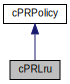
\includegraphics[width=142pt]{d9/da4/classcPRLru__inherit__graph}
\end{center}
\end{figure}


\-Collaboration diagram for c\-P\-R\-Lru\-:\nopagebreak
\begin{figure}[H]
\begin{center}
\leavevmode
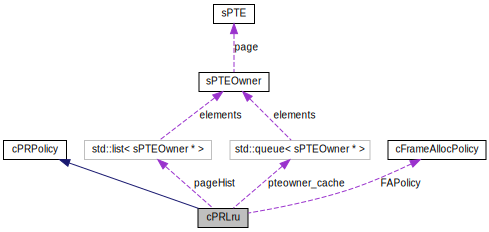
\includegraphics[width=350pt]{da/d0b/classcPRLru__coll__graph}
\end{center}
\end{figure}
\subsection*{\-Public \-Member \-Functions}
\begin{DoxyCompactItemize}
\item 
\hypertarget{classcPRLru_a483b47a8f7a83e63fb4a7d02d1b1ba91}{{\bfseries c\-P\-R\-Lru} (\hyperlink{classcFrameAllocPolicy}{c\-Frame\-Alloc\-Policy} \&\-\_\-\-F\-A\-Policy)}\label{da/da5/classcPRLru_a483b47a8f7a83e63fb4a7d02d1b1ba91}

\item 
const char $\ast$ \hyperlink{classcPRLru_aec12730888e052c697b43ed8aca4b8a6}{name} ()
\begin{DoxyCompactList}\small\item\em \-Name of \-P\-R module. \end{DoxyCompactList}\item 
\hyperlink{pageReplace_8h_af4bc4c41a44c2bd80e8cbf1aae370217}{e\-P\-R\-Status} \hyperlink{classcPRLru_aab495ba087dfd717fd9908fb138069bc}{resolve\-Page\-Fault} (\hyperlink{structsProc}{s\-Proc} $\ast$proc, uint32\-\_\-t page)
\begin{DoxyCompactList}\small\item\em \-If no frames are free, spill the frame that has the lowest timestamp, or was "least recently used. \end{DoxyCompactList}\item 
\hypertarget{classcPRLru_a9e0bb304978dddc8342a5b9445c091b6}{void \hyperlink{classcPRLru_a9e0bb304978dddc8342a5b9445c091b6}{finished\-Quanta} (\hyperlink{structsProc}{s\-Proc} $\ast$proc)}\label{da/da5/classcPRLru_a9e0bb304978dddc8342a5b9445c091b6}

\begin{DoxyCompactList}\small\item\em \-Since all the times are set in software, this method does nothing. \end{DoxyCompactList}\item 
\hypertarget{classcPRLru_a003230ac7e50911cfa74808ffeefa658}{void \hyperlink{classcPRLru_a003230ac7e50911cfa74808ffeefa658}{finished\-I\-O} (\hyperlink{structsProc}{s\-Proc} $\ast$proc, \hyperlink{structsPTE}{s\-P\-T\-E} $\ast$page)}\label{da/da5/classcPRLru_a003230ac7e50911cfa74808ffeefa658}

\begin{DoxyCompactList}\small\item\em \-Add the \-P\-T\-E to the page\-Hist to keep track of which frames have been given out. \end{DoxyCompactList}\item 
\hypertarget{classcPRLru_ae74d5e116ffad469d9f6417034f4b0d6}{bool \hyperlink{classcPRLru_ae74d5e116ffad469d9f6417034f4b0d6}{clear\-Pages} (int num\-Pages)}\label{da/da5/classcPRLru_ae74d5e116ffad469d9f6417034f4b0d6}

\begin{DoxyCompactList}\small\item\em \-Sorts page\-Hist by timestamp (increasing order) then removes num\-Pages from the front of the list. \end{DoxyCompactList}\item 
\hypertarget{classcPRLru_a6ab14eaa8e52cf40ca9921bad685d1d2}{void \hyperlink{classcPRLru_a6ab14eaa8e52cf40ca9921bad685d1d2}{unpin\-Frame} (uint32\-\_\-t frame)}\label{da/da5/classcPRLru_a6ab14eaa8e52cf40ca9921bad685d1d2}

\begin{DoxyCompactList}\small\item\em \-This is typically called after \-::finished\-I\-O so that the \-P\-R module unpins the frame in the frame allocation module. \end{DoxyCompactList}\item 
void \hyperlink{classcPRLru_a9ab0ecc8f28bb2643bfe06cc11f4abb7}{print\-Timestamps} ()
\begin{DoxyCompactList}\small\item\em \-Used for debugging purposes. \end{DoxyCompactList}\item 
void \hyperlink{classcPRLru_a50542682b40a9a5fc48506a347e70c53}{return\-Frame} (uint32\-\_\-t frame)
\begin{DoxyCompactList}\small\item\em \-Return a frame to the system. \end{DoxyCompactList}\end{DoxyCompactItemize}
\subsection*{\-Private \-Member \-Functions}
\begin{DoxyCompactItemize}
\item 
\hyperlink{structsPTEOwner}{s\-P\-T\-E\-Owner} $\ast$ \hyperlink{classcPRLru_a87be0bcf2c296b41d66f3a419d53fa98}{get\-P\-T\-E\-Owner} ()
\begin{DoxyCompactList}\small\item\em \-Get a struct for holding both the \-P\-T\-E and \-Owner. \end{DoxyCompactList}\item 
\hypertarget{classcPRLru_a892e3d84ca361766506ed3615d3dddd8}{void \hyperlink{classcPRLru_a892e3d84ca361766506ed3615d3dddd8}{return\-P\-T\-E\-Owner} (\hyperlink{structsPTEOwner}{s\-P\-T\-E\-Owner} $\ast$pte\-Owner)}\label{da/da5/classcPRLru_a892e3d84ca361766506ed3615d3dddd8}

\begin{DoxyCompactList}\small\item\em \-Add a \-P\-T\-E\-Owner to the pteowner\-\_\-cache to use later. \end{DoxyCompactList}\end{DoxyCompactItemize}
\subsection*{\-Private \-Attributes}
\begin{DoxyCompactItemize}
\item 
\hypertarget{classcPRLru_aecc5ad74db574fe06501fad7eeb930a2}{list$<$ \hyperlink{structsPTEOwner}{s\-P\-T\-E\-Owner} $\ast$ $>$ {\bfseries page\-Hist}}\label{da/da5/classcPRLru_aecc5ad74db574fe06501fad7eeb930a2}

\item 
\hypertarget{classcPRLru_a790a6f44fd2d54b5580acf624604bee6}{queue$<$ \hyperlink{structsPTEOwner}{s\-P\-T\-E\-Owner} $\ast$ $>$ {\bfseries pteowner\-\_\-cache}}\label{da/da5/classcPRLru_a790a6f44fd2d54b5580acf624604bee6}

\item 
\hypertarget{classcPRLru_a55b7edeffaf80911b7b3aba7aa422b83}{\hyperlink{classcFrameAllocPolicy}{c\-Frame\-Alloc\-Policy} \& {\bfseries \-F\-A\-Policy}}\label{da/da5/classcPRLru_a55b7edeffaf80911b7b3aba7aa422b83}

\item 
\hypertarget{classcPRLru_a04cbd077d45c2183f6d61dde9f03ad14}{uint32\-\_\-t {\bfseries \-P\-T\-Size}}\label{da/da5/classcPRLru_a04cbd077d45c2183f6d61dde9f03ad14}

\end{DoxyCompactItemize}


\subsection{\-Member \-Function \-Documentation}
\hypertarget{classcPRLru_a87be0bcf2c296b41d66f3a419d53fa98}{\index{c\-P\-R\-Lru@{c\-P\-R\-Lru}!get\-P\-T\-E\-Owner@{get\-P\-T\-E\-Owner}}
\index{get\-P\-T\-E\-Owner@{get\-P\-T\-E\-Owner}!cPRLru@{c\-P\-R\-Lru}}
\subsubsection[{get\-P\-T\-E\-Owner}]{\setlength{\rightskip}{0pt plus 5cm}{\bf s\-P\-T\-E\-Owner} $\ast$ {\bf c\-P\-R\-Lru\-::get\-P\-T\-E\-Owner} (
\begin{DoxyParamCaption}
{}
\end{DoxyParamCaption}
)\hspace{0.3cm}{\ttfamily  \mbox{[}private\mbox{]}}}}\label{da/da5/classcPRLru_a87be0bcf2c296b41d66f3a419d53fa98}
\-If the pteowner\-\_\-cache has an entry, re-\/use it. \-Otherwise malloc a new one. \-This helps with heap performance. 

\-Referenced by finished\-I\-O().

\hypertarget{classcPRLru_aec12730888e052c697b43ed8aca4b8a6}{\index{c\-P\-R\-Lru@{c\-P\-R\-Lru}!name@{name}}
\index{name@{name}!cPRLru@{c\-P\-R\-Lru}}
\subsubsection[{name}]{\setlength{\rightskip}{0pt plus 5cm}const char$\ast$ {\bf c\-P\-R\-Lru\-::name} (
\begin{DoxyParamCaption}
{}
\end{DoxyParamCaption}
)\hspace{0.3cm}{\ttfamily  \mbox{[}inline, virtual\mbox{]}}}}\label{da/da5/classcPRLru_aec12730888e052c697b43ed8aca4b8a6}
\-This is only used for logging purposes so that the \-P\-R module can be easily identified. 

\-Implements \hyperlink{classcPRPolicy_ad0de8c0c77f8d2ecb1f5679f0c25b5be}{c\-P\-R\-Policy}.

\hypertarget{classcPRLru_a9ab0ecc8f28bb2643bfe06cc11f4abb7}{\index{c\-P\-R\-Lru@{c\-P\-R\-Lru}!print\-Timestamps@{print\-Timestamps}}
\index{print\-Timestamps@{print\-Timestamps}!cPRLru@{c\-P\-R\-Lru}}
\subsubsection[{print\-Timestamps}]{\setlength{\rightskip}{0pt plus 5cm}void {\bf c\-P\-R\-Lru\-::print\-Timestamps} (
\begin{DoxyParamCaption}
{}
\end{DoxyParamCaption}
)}}\label{da/da5/classcPRLru_a9ab0ecc8f28bb2643bfe06cc11f4abb7}
\-Prints all of the timestamps in the page\-Hist list. \hypertarget{classcPRLru_aab495ba087dfd717fd9908fb138069bc}{\index{c\-P\-R\-Lru@{c\-P\-R\-Lru}!resolve\-Page\-Fault@{resolve\-Page\-Fault}}
\index{resolve\-Page\-Fault@{resolve\-Page\-Fault}!cPRLru@{c\-P\-R\-Lru}}
\subsubsection[{resolve\-Page\-Fault}]{\setlength{\rightskip}{0pt plus 5cm}{\bf e\-P\-R\-Status} {\bf c\-P\-R\-Lru\-::resolve\-Page\-Fault} (
\begin{DoxyParamCaption}
\item[{{\bf s\-Proc} $\ast$}]{proc, }
\item[{uint32\-\_\-t}]{page}
\end{DoxyParamCaption}
)\hspace{0.3cm}{\ttfamily  \mbox{[}virtual\mbox{]}}}}\label{da/da5/classcPRLru_aab495ba087dfd717fd9908fb138069bc}
" 

\-Implements \hyperlink{classcPRPolicy_aae8a15e6e99ec90d54210fc4d4ddf211}{c\-P\-R\-Policy}.

\hypertarget{classcPRLru_a50542682b40a9a5fc48506a347e70c53}{\index{c\-P\-R\-Lru@{c\-P\-R\-Lru}!return\-Frame@{return\-Frame}}
\index{return\-Frame@{return\-Frame}!cPRLru@{c\-P\-R\-Lru}}
\subsubsection[{return\-Frame}]{\setlength{\rightskip}{0pt plus 5cm}void {\bf c\-P\-R\-Lru\-::return\-Frame} (
\begin{DoxyParamCaption}
\item[{uint32\-\_\-t}]{frame}
\end{DoxyParamCaption}
)\hspace{0.3cm}{\ttfamily  \mbox{[}virtual\mbox{]}}}}\label{da/da5/classcPRLru_a50542682b40a9a5fc48506a347e70c53}
\-The \-V\-M\-M core calls this when a process termintates to free up any of its used frames. \-This call could be made directly to the frame allocator but using the \-P\-R module as a middle man gives it a chance to update as needed. 

\-Implements \hyperlink{classcPRPolicy_ac78fc5c56b8f485eb18f6f36968612f1}{c\-P\-R\-Policy}.



\-The documentation for this class was generated from the following files\-:\begin{DoxyCompactItemize}
\item 
include/\-Policy/pr\-\_\-lru.\-h\item 
src/\-Policy/pr\-\_\-lru.\-cpp\end{DoxyCompactItemize}

\hypertarget{classcPRLruApprox}{\section{c\-P\-R\-Lru\-Approx \-Class \-Reference}
\label{d1/d58/classcPRLruApprox}\index{c\-P\-R\-Lru\-Approx@{c\-P\-R\-Lru\-Approx}}
}


\-Inheritance diagram for c\-P\-R\-Lru\-Approx\-:\nopagebreak
\begin{figure}[H]
\begin{center}
\leavevmode
\includegraphics[width=160pt]{d2/d0a/classcPRLruApprox__inherit__graph}
\end{center}
\end{figure}


\-Collaboration diagram for c\-P\-R\-Lru\-Approx\-:\nopagebreak
\begin{figure}[H]
\begin{center}
\leavevmode
\includegraphics[width=350pt]{d0/d7d/classcPRLruApprox__coll__graph}
\end{center}
\end{figure}
\subsection*{\-Public \-Member \-Functions}
\begin{DoxyCompactItemize}
\item 
\hypertarget{classcPRLruApprox_afd0d2b59608725365a49418ac479ad00}{{\bfseries c\-P\-R\-Lru\-Approx} (\hyperlink{classcFrameAllocPolicy}{c\-Frame\-Alloc\-Policy} \&\-\_\-\-F\-A\-Policy)}\label{d1/d58/classcPRLruApprox_afd0d2b59608725365a49418ac479ad00}

\item 
const char $\ast$ \hyperlink{classcPRLruApprox_acf51ca9d36ab017456f856809e13dab7}{name} ()
\begin{DoxyCompactList}\small\item\em \-Name of \-P\-R module. \end{DoxyCompactList}\item 
\hyperlink{pageReplace_8h_af4bc4c41a44c2bd80e8cbf1aae370217}{e\-P\-R\-Status} \hyperlink{classcPRLruApprox_adc2d729279fec03798c9027c87af7c84}{resolve\-Page\-Fault} (\hyperlink{structsProc}{s\-Proc} $\ast$proc, uint32\-\_\-t page)
\begin{DoxyCompactList}\small\item\em \-If no frames are free, spill the frame that has the lowest shifted time. \end{DoxyCompactList}\item 
\hypertarget{classcPRLruApprox_aaf6600b3edb01fbbb0257f622b3fb1ec}{void \hyperlink{classcPRLruApprox_aaf6600b3edb01fbbb0257f622b3fb1ec}{finished\-Quanta} (\hyperlink{structsProc}{s\-Proc} $\ast$proc)}\label{d1/d58/classcPRLruApprox_aaf6600b3edb01fbbb0257f622b3fb1ec}

\begin{DoxyCompactList}\small\item\em \-Update the approx time field in software. \end{DoxyCompactList}\item 
\hypertarget{classcPRLruApprox_a93c48941ed2511000566bb3d24cf8313}{void \hyperlink{classcPRLruApprox_a93c48941ed2511000566bb3d24cf8313}{finished\-I\-O} (\hyperlink{structsProc}{s\-Proc} $\ast$proc, \hyperlink{structsPTE}{s\-P\-T\-E} $\ast$page)}\label{d1/d58/classcPRLruApprox_a93c48941ed2511000566bb3d24cf8313}

\begin{DoxyCompactList}\small\item\em \-I/\-O is finished so add the \-P\-T\-E to the page\-Hist so we know what frames are in use. \end{DoxyCompactList}\item 
bool \hyperlink{classcPRLruApprox_a7b1d7330af067ad28c089fb7a6267c00}{clear\-Pages} (int num\-Pages)
\begin{DoxyCompactList}\small\item\em \-Clears pages by sorting the page\-Hist by the time field (increasing). \end{DoxyCompactList}\item 
\hypertarget{classcPRLruApprox_aa14da3923094c008b82a07f430d97c19}{void \hyperlink{classcPRLruApprox_aa14da3923094c008b82a07f430d97c19}{unpin\-Frame} (uint32\-\_\-t frame)}\label{d1/d58/classcPRLruApprox_aa14da3923094c008b82a07f430d97c19}

\begin{DoxyCompactList}\small\item\em \-This is typically called after \-::finished\-I\-O so that the \-P\-R module unpins the frame in the frame allocation module. \end{DoxyCompactList}\item 
void \hyperlink{classcPRLruApprox_a5cc1b3cbc08b1ef334eb37138ff95c43}{return\-Frame} (uint32\-\_\-t frame)
\begin{DoxyCompactList}\small\item\em \-Return a frame to the system. \end{DoxyCompactList}\end{DoxyCompactItemize}
\subsection*{\-Private \-Member \-Functions}
\begin{DoxyCompactItemize}
\item 
void \hyperlink{classcPRLruApprox_a72c71139928164b0c300c3c2b0bb89f9}{update\-Time} ()
\begin{DoxyCompactList}\small\item\em \-Updates the time field by first shifting the time field to the right and then adding a 1 in the far left position if the ref bit is set. \end{DoxyCompactList}\item 
\hyperlink{structsPTEOwner}{s\-P\-T\-E\-Owner} $\ast$ \hyperlink{classcPRLruApprox_aa3b208b716158d929a314a1362e1b9e4}{get\-P\-T\-E\-Owner} ()
\begin{DoxyCompactList}\small\item\em \-Get a struct for holding both the \-P\-T\-E and \-Owner. \end{DoxyCompactList}\item 
\hypertarget{classcPRLruApprox_a9df7f4858418f4e8d61e38d56ec66d9d}{void \hyperlink{classcPRLruApprox_a9df7f4858418f4e8d61e38d56ec66d9d}{return\-P\-T\-E\-Owner} (\hyperlink{structsPTEOwner}{s\-P\-T\-E\-Owner} $\ast$pte\-Owner)}\label{d1/d58/classcPRLruApprox_a9df7f4858418f4e8d61e38d56ec66d9d}

\begin{DoxyCompactList}\small\item\em \-Add a \-P\-T\-E\-Owner to the pteowner\-\_\-cache to use later. \end{DoxyCompactList}\end{DoxyCompactItemize}
\subsection*{\-Private \-Attributes}
\begin{DoxyCompactItemize}
\item 
\hypertarget{classcPRLruApprox_a4514e3036505b6f3d30b3af0e8e304e9}{list$<$ \hyperlink{structsPTEOwner}{s\-P\-T\-E\-Owner} $\ast$ $>$ {\bfseries page\-Hist}}\label{d1/d58/classcPRLruApprox_a4514e3036505b6f3d30b3af0e8e304e9}

\item 
\hypertarget{classcPRLruApprox_a499f2e4b2930777879e95c531eac4adf}{queue$<$ \hyperlink{structsPTEOwner}{s\-P\-T\-E\-Owner} $\ast$ $>$ {\bfseries pteowner\-\_\-cache}}\label{d1/d58/classcPRLruApprox_a499f2e4b2930777879e95c531eac4adf}

\item 
\hypertarget{classcPRLruApprox_a8ceefcbdbed074f0a66e875e6d25ed34}{\hyperlink{classcFrameAllocPolicy}{c\-Frame\-Alloc\-Policy} \& {\bfseries \-F\-A\-Policy}}\label{d1/d58/classcPRLruApprox_a8ceefcbdbed074f0a66e875e6d25ed34}

\item 
\hypertarget{classcPRLruApprox_a428819ec4906eb67b1bc34dc3bf09608}{uint32\-\_\-t {\bfseries \-P\-T\-Size}}\label{d1/d58/classcPRLruApprox_a428819ec4906eb67b1bc34dc3bf09608}

\end{DoxyCompactItemize}


\subsection{\-Member \-Function \-Documentation}
\hypertarget{classcPRLruApprox_a7b1d7330af067ad28c089fb7a6267c00}{\index{c\-P\-R\-Lru\-Approx@{c\-P\-R\-Lru\-Approx}!clear\-Pages@{clear\-Pages}}
\index{clear\-Pages@{clear\-Pages}!cPRLruApprox@{c\-P\-R\-Lru\-Approx}}
\subsubsection[{clear\-Pages}]{\setlength{\rightskip}{0pt plus 5cm}bool {\bf c\-P\-R\-Lru\-Approx\-::clear\-Pages} (
\begin{DoxyParamCaption}
\item[{int}]{num\-Pages}
\end{DoxyParamCaption}
)\hspace{0.3cm}{\ttfamily  \mbox{[}virtual\mbox{]}}}}\label{d1/d58/classcPRLruApprox_a7b1d7330af067ad28c089fb7a6267c00}
\-Then removes num\-Pages from the front of page\-Hist. 

\-Implements \hyperlink{classcPRPolicy_a7a2b6d5761963a69d20794579d39530f}{c\-P\-R\-Policy}.

\hypertarget{classcPRLruApprox_aa3b208b716158d929a314a1362e1b9e4}{\index{c\-P\-R\-Lru\-Approx@{c\-P\-R\-Lru\-Approx}!get\-P\-T\-E\-Owner@{get\-P\-T\-E\-Owner}}
\index{get\-P\-T\-E\-Owner@{get\-P\-T\-E\-Owner}!cPRLruApprox@{c\-P\-R\-Lru\-Approx}}
\subsubsection[{get\-P\-T\-E\-Owner}]{\setlength{\rightskip}{0pt plus 5cm}{\bf s\-P\-T\-E\-Owner} $\ast$ {\bf c\-P\-R\-Lru\-Approx\-::get\-P\-T\-E\-Owner} (
\begin{DoxyParamCaption}
{}
\end{DoxyParamCaption}
)\hspace{0.3cm}{\ttfamily  \mbox{[}private\mbox{]}}}}\label{d1/d58/classcPRLruApprox_aa3b208b716158d929a314a1362e1b9e4}
\-If the pteowner\-\_\-cache has an entry, re-\/use it. \-Otherwise malloc a new one. \-This helps with heap performance. 

\-Referenced by finished\-I\-O().

\hypertarget{classcPRLruApprox_acf51ca9d36ab017456f856809e13dab7}{\index{c\-P\-R\-Lru\-Approx@{c\-P\-R\-Lru\-Approx}!name@{name}}
\index{name@{name}!cPRLruApprox@{c\-P\-R\-Lru\-Approx}}
\subsubsection[{name}]{\setlength{\rightskip}{0pt plus 5cm}const char$\ast$ {\bf c\-P\-R\-Lru\-Approx\-::name} (
\begin{DoxyParamCaption}
{}
\end{DoxyParamCaption}
)\hspace{0.3cm}{\ttfamily  \mbox{[}inline, virtual\mbox{]}}}}\label{d1/d58/classcPRLruApprox_acf51ca9d36ab017456f856809e13dab7}
\-This is only used for logging purposes so that the \-P\-R module can be easily identified. 

\-Implements \hyperlink{classcPRPolicy_ad0de8c0c77f8d2ecb1f5679f0c25b5be}{c\-P\-R\-Policy}.

\hypertarget{classcPRLruApprox_adc2d729279fec03798c9027c87af7c84}{\index{c\-P\-R\-Lru\-Approx@{c\-P\-R\-Lru\-Approx}!resolve\-Page\-Fault@{resolve\-Page\-Fault}}
\index{resolve\-Page\-Fault@{resolve\-Page\-Fault}!cPRLruApprox@{c\-P\-R\-Lru\-Approx}}
\subsubsection[{resolve\-Page\-Fault}]{\setlength{\rightskip}{0pt plus 5cm}{\bf e\-P\-R\-Status} {\bf c\-P\-R\-Lru\-Approx\-::resolve\-Page\-Fault} (
\begin{DoxyParamCaption}
\item[{{\bf s\-Proc} $\ast$}]{proc, }
\item[{uint32\-\_\-t}]{page}
\end{DoxyParamCaption}
)\hspace{0.3cm}{\ttfamily  \mbox{[}virtual\mbox{]}}}}\label{d1/d58/classcPRLruApprox_adc2d729279fec03798c9027c87af7c84}
\-This aging algorithm simulates \-L\-R\-U. 

\-Implements \hyperlink{classcPRPolicy_aae8a15e6e99ec90d54210fc4d4ddf211}{c\-P\-R\-Policy}.

\hypertarget{classcPRLruApprox_a5cc1b3cbc08b1ef334eb37138ff95c43}{\index{c\-P\-R\-Lru\-Approx@{c\-P\-R\-Lru\-Approx}!return\-Frame@{return\-Frame}}
\index{return\-Frame@{return\-Frame}!cPRLruApprox@{c\-P\-R\-Lru\-Approx}}
\subsubsection[{return\-Frame}]{\setlength{\rightskip}{0pt plus 5cm}void {\bf c\-P\-R\-Lru\-Approx\-::return\-Frame} (
\begin{DoxyParamCaption}
\item[{uint32\-\_\-t}]{frame}
\end{DoxyParamCaption}
)\hspace{0.3cm}{\ttfamily  \mbox{[}virtual\mbox{]}}}}\label{d1/d58/classcPRLruApprox_a5cc1b3cbc08b1ef334eb37138ff95c43}
\-The \-V\-M\-M core calls this when a process termintates to free up any of its used frames. \-This call could be made directly to the frame allocator but using the \-P\-R module as a middle man gives it a chance to update as needed. 

\-Implements \hyperlink{classcPRPolicy_ac78fc5c56b8f485eb18f6f36968612f1}{c\-P\-R\-Policy}.

\hypertarget{classcPRLruApprox_a72c71139928164b0c300c3c2b0bb89f9}{\index{c\-P\-R\-Lru\-Approx@{c\-P\-R\-Lru\-Approx}!update\-Time@{update\-Time}}
\index{update\-Time@{update\-Time}!cPRLruApprox@{c\-P\-R\-Lru\-Approx}}
\subsubsection[{update\-Time}]{\setlength{\rightskip}{0pt plus 5cm}{\bf c\-P\-R\-Lru\-Approx\-::update\-Time} (
\begin{DoxyParamCaption}
{}
\end{DoxyParamCaption}
)\hspace{0.3cm}{\ttfamily  \mbox{[}private\mbox{]}}}}\label{d1/d58/classcPRLruApprox_a72c71139928164b0c300c3c2b0bb89f9}
\-This function is called on a page fault or after a quanta is finished. 

\-Referenced by finished\-Quanta(), and resolve\-Page\-Fault().



\-The documentation for this class was generated from the following files\-:\begin{DoxyCompactItemize}
\item 
include/\-Policy/pr\-\_\-lru\-Approx.\-h\item 
src/\-Policy/pr\-\_\-lru\-Approx.\-cpp\end{DoxyCompactItemize}

\hypertarget{classcPRPolicy}{\section{c\-P\-R\-Policy \-Class \-Reference}
\label{d7/df0/classcPRPolicy}\index{c\-P\-R\-Policy@{c\-P\-R\-Policy}}
}


\-Abstract \-Page \-Replacement \-Policy.  




{\ttfamily \#include $<$page\-Replace.\-h$>$}



\-Inheritance diagram for c\-P\-R\-Policy\-:\nopagebreak
\begin{figure}[H]
\begin{center}
\leavevmode
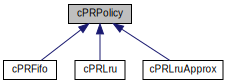
\includegraphics[width=299pt]{d6/d74/classcPRPolicy__inherit__graph}
\end{center}
\end{figure}
\subsection*{\-Public \-Member \-Functions}
\begin{DoxyCompactItemize}
\item 
\hypertarget{classcPRPolicy_ad100e742a4a0442512c1196d657e4b28}{{\bfseries c\-P\-R\-Policy} (\hyperlink{classcFrameAllocPolicy}{c\-Frame\-Alloc\-Policy} \&)}\label{d7/df0/classcPRPolicy_ad100e742a4a0442512c1196d657e4b28}

\item 
virtual const char $\ast$ \hyperlink{classcPRPolicy_ad0de8c0c77f8d2ecb1f5679f0c25b5be}{name} ()=0
\begin{DoxyCompactList}\small\item\em \-Name of \-P\-R module. \end{DoxyCompactList}\item 
virtual \hyperlink{pageReplace_8h_af4bc4c41a44c2bd80e8cbf1aae370217}{e\-P\-R\-Status} \hyperlink{classcPRPolicy_aae8a15e6e99ec90d54210fc4d4ddf211}{resolve\-Page\-Fault} (\hyperlink{structsProc}{s\-Proc} $\ast$proc, uint32\-\_\-t page)=0
\begin{DoxyCompactList}\small\item\em \-Get a page frame for this process. \end{DoxyCompactList}\item 
\hypertarget{classcPRPolicy_a21eaa5302ec87c7643eb2c0d0f65f5cf}{\hyperlink{pageReplace_8h_af4bc4c41a44c2bd80e8cbf1aae370217}{e\-P\-R\-Status} {\bfseries resolve\-Circular\-P\-F} (\hyperlink{structsProc}{s\-Proc} $\ast$proc, uint32\-\_\-t page)}\label{d7/df0/classcPRPolicy_a21eaa5302ec87c7643eb2c0d0f65f5cf}

\item 
virtual void \hyperlink{classcPRPolicy_adfe4408f052b6ec414331ba1bafc736b}{finished\-Quanta} (\hyperlink{structsProc}{s\-Proc} $\ast$)=0
\begin{DoxyCompactList}\small\item\em \-This is called after an execution quanta finishes. \end{DoxyCompactList}\item 
virtual void \hyperlink{classcPRPolicy_a169fb952830fa103a72a1cd223ac081f}{finished\-I\-O} (\hyperlink{structsProc}{s\-Proc} $\ast$, \hyperlink{structsPTE}{s\-P\-T\-E} $\ast$)=0
\begin{DoxyCompactList}\small\item\em \-This is called after an \-I/\-O (input) completes. \end{DoxyCompactList}\item 
virtual bool \hyperlink{classcPRPolicy_a7a2b6d5761963a69d20794579d39530f}{clear\-Pages} (int num\-Pages)=0
\begin{DoxyCompactList}\small\item\em \-Remove this many pages from memory. \end{DoxyCompactList}\item 
\hypertarget{classcPRPolicy_a8ef7dce4fcf989f6aa212920055fa4bb}{virtual void \hyperlink{classcPRPolicy_a8ef7dce4fcf989f6aa212920055fa4bb}{unpin\-Frame} (uint32\-\_\-t frame)=0}\label{d7/df0/classcPRPolicy_a8ef7dce4fcf989f6aa212920055fa4bb}

\begin{DoxyCompactList}\small\item\em \-This is typically called after \-::finished\-I\-O so that the \-P\-R module unpins the frame in the frame allocation module. \end{DoxyCompactList}\item 
virtual void \hyperlink{classcPRPolicy_ac78fc5c56b8f485eb18f6f36968612f1}{return\-Frame} (uint32\-\_\-t frame)=0
\begin{DoxyCompactList}\small\item\em \-Return this frame to the system. \end{DoxyCompactList}\end{DoxyCompactItemize}


\subsection{\-Member \-Function \-Documentation}
\hypertarget{classcPRPolicy_a7a2b6d5761963a69d20794579d39530f}{\index{c\-P\-R\-Policy@{c\-P\-R\-Policy}!clear\-Pages@{clear\-Pages}}
\index{clear\-Pages@{clear\-Pages}!cPRPolicy@{c\-P\-R\-Policy}}
\subsubsection[{clear\-Pages}]{\setlength{\rightskip}{0pt plus 5cm}{\bf c\-P\-R\-Policy\-::clear\-Pages} (
\begin{DoxyParamCaption}
\item[{int}]{num\-Pages}
\end{DoxyParamCaption}
)\hspace{0.3cm}{\ttfamily  \mbox{[}pure virtual\mbox{]}}}}\label{d7/df0/classcPRPolicy_a7a2b6d5761963a69d20794579d39530f}
\-If the cleaning daemon decides that pages need to be cleaned it will determine how many from its policy and call the \-P\-R module to clean that many. \-This method keeps the \-P\-R policy separate from the decision on how many pages to clean and when.


\begin{DoxyParams}{\-Parameters}
{\em int} & \-Number of pages to clear. \\
\hline
\end{DoxyParams}


\-Implemented in \hyperlink{classcPRLru_ae74d5e116ffad469d9f6417034f4b0d6}{c\-P\-R\-Lru}, \hyperlink{classcPRLruApprox_a7b1d7330af067ad28c089fb7a6267c00}{c\-P\-R\-Lru\-Approx}, and \hyperlink{classcPRFifo_ab2bca492cfd0a628df492781ecd726ff}{c\-P\-R\-Fifo}.



\-Referenced by c\-V\-M\-M\-::start().

\hypertarget{classcPRPolicy_a169fb952830fa103a72a1cd223ac081f}{\index{c\-P\-R\-Policy@{c\-P\-R\-Policy}!finished\-I\-O@{finished\-I\-O}}
\index{finished\-I\-O@{finished\-I\-O}!cPRPolicy@{c\-P\-R\-Policy}}
\subsubsection[{finished\-I\-O}]{\setlength{\rightskip}{0pt plus 5cm}{\bf c\-P\-R\-Policy\-::finished\-I\-O} (
\begin{DoxyParamCaption}
\item[{{\bf s\-Proc} $\ast$}]{, }
\item[{{\bf s\-P\-T\-E} $\ast$}]{}
\end{DoxyParamCaption}
)\hspace{0.3cm}{\ttfamily  \mbox{[}pure virtual\mbox{]}}}}\label{d7/df0/classcPRPolicy_a169fb952830fa103a72a1cd223ac081f}
\-This is another notification point for the \-P\-R module to update its data structs. 

\-Implemented in \hyperlink{classcPRLru_a003230ac7e50911cfa74808ffeefa658}{c\-P\-R\-Lru}, \hyperlink{classcPRLruApprox_a93c48941ed2511000566bb3d24cf8313}{c\-P\-R\-Lru\-Approx}, and \hyperlink{classcPRFifo_a158824c0cf38fa23a14f7148431bc34d}{c\-P\-R\-Fifo}.



\-Referenced by c\-V\-M\-M\-::start().

\hypertarget{classcPRPolicy_adfe4408f052b6ec414331ba1bafc736b}{\index{c\-P\-R\-Policy@{c\-P\-R\-Policy}!finished\-Quanta@{finished\-Quanta}}
\index{finished\-Quanta@{finished\-Quanta}!cPRPolicy@{c\-P\-R\-Policy}}
\subsubsection[{finished\-Quanta}]{\setlength{\rightskip}{0pt plus 5cm}{\bf c\-P\-R\-Policy\-::finished\-Quanta} (
\begin{DoxyParamCaption}
\item[{{\bf s\-Proc} $\ast$}]{}
\end{DoxyParamCaption}
)\hspace{0.3cm}{\ttfamily  \mbox{[}pure virtual\mbox{]}}}}\label{d7/df0/classcPRPolicy_adfe4408f052b6ec414331ba1bafc736b}
\-This gives the \-P\-R module a chance to update its internal data-\/structures using the reference bits or any other data available from the process struct. 

\-Implemented in \hyperlink{classcPRLru_a9e0bb304978dddc8342a5b9445c091b6}{c\-P\-R\-Lru}, \hyperlink{classcPRLruApprox_aaf6600b3edb01fbbb0257f622b3fb1ec}{c\-P\-R\-Lru\-Approx}, and \hyperlink{classcPRFifo_aadb8319e6e539280e0f56c0e6b40c581}{c\-P\-R\-Fifo}.



\-Referenced by c\-V\-M\-M\-::start().

\hypertarget{classcPRPolicy_ad0de8c0c77f8d2ecb1f5679f0c25b5be}{\index{c\-P\-R\-Policy@{c\-P\-R\-Policy}!name@{name}}
\index{name@{name}!cPRPolicy@{c\-P\-R\-Policy}}
\subsubsection[{name}]{\setlength{\rightskip}{0pt plus 5cm}virtual const char$\ast$ {\bf c\-P\-R\-Policy\-::name} (
\begin{DoxyParamCaption}
{}
\end{DoxyParamCaption}
)\hspace{0.3cm}{\ttfamily  \mbox{[}pure virtual\mbox{]}}}}\label{d7/df0/classcPRPolicy_ad0de8c0c77f8d2ecb1f5679f0c25b5be}
\-This is only used for logging purposes so that the \-P\-R module can be easily identified. 

\-Implemented in \hyperlink{classcPRLruApprox_acf51ca9d36ab017456f856809e13dab7}{c\-P\-R\-Lru\-Approx}, \hyperlink{classcPRLru_aec12730888e052c697b43ed8aca4b8a6}{c\-P\-R\-Lru}, and \hyperlink{classcPRFifo_aa3b9269589ccebd364d07ef69015bad6}{c\-P\-R\-Fifo}.



\-Referenced by c\-V\-M\-M\-::print\-Results().

\hypertarget{classcPRPolicy_aae8a15e6e99ec90d54210fc4d4ddf211}{\index{c\-P\-R\-Policy@{c\-P\-R\-Policy}!resolve\-Page\-Fault@{resolve\-Page\-Fault}}
\index{resolve\-Page\-Fault@{resolve\-Page\-Fault}!cPRPolicy@{c\-P\-R\-Policy}}
\subsubsection[{resolve\-Page\-Fault}]{\setlength{\rightskip}{0pt plus 5cm}virtual {\bf e\-P\-R\-Status} {\bf c\-P\-R\-Policy\-::resolve\-Page\-Fault} (
\begin{DoxyParamCaption}
\item[{{\bf s\-Proc} $\ast$}]{proc, }
\item[{uint32\-\_\-t}]{page}
\end{DoxyParamCaption}
)\hspace{0.3cm}{\ttfamily  \mbox{[}pure virtual\mbox{]}}}}\label{d7/df0/classcPRPolicy_aae8a15e6e99ec90d54210fc4d4ddf211}
\-If a free one is available from the frame allocator it will be used. \-Otherwise, a page will have to be spilled.


\begin{DoxyParams}{\-Parameters}
{\em s\-Proc$\ast$} & \-A pointer to the process that the frame is being requested for.\\
\hline
{\em uint32\-\_\-t} & page \-The page for the given process that needs to be fetched. \\
\hline
\end{DoxyParams}


\-Implemented in \hyperlink{classcPRLru_aab495ba087dfd717fd9908fb138069bc}{c\-P\-R\-Lru}, \hyperlink{classcPRLruApprox_adc2d729279fec03798c9027c87af7c84}{c\-P\-R\-Lru\-Approx}, and \hyperlink{classcPRFifo_a8121128a2dac3c8194c044e81fa0e5fc}{c\-P\-R\-Fifo}.



\-Referenced by c\-V\-M\-M\-::start().

\hypertarget{classcPRPolicy_ac78fc5c56b8f485eb18f6f36968612f1}{\index{c\-P\-R\-Policy@{c\-P\-R\-Policy}!return\-Frame@{return\-Frame}}
\index{return\-Frame@{return\-Frame}!cPRPolicy@{c\-P\-R\-Policy}}
\subsubsection[{return\-Frame}]{\setlength{\rightskip}{0pt plus 5cm}{\bf c\-P\-R\-Policy\-::return\-Frame} (
\begin{DoxyParamCaption}
\item[{uint32\-\_\-t}]{frame}
\end{DoxyParamCaption}
)\hspace{0.3cm}{\ttfamily  \mbox{[}pure virtual\mbox{]}}}}\label{d7/df0/classcPRPolicy_ac78fc5c56b8f485eb18f6f36968612f1}
\-This is called when a process exits and its frames are being returned to the system. \-This is usually a wrapper to the \-F\-A policy return frame function but it gives the \-P\-R module a chance to update its datastructures if necessary.

\-Since we have made the assumption that this is only called on process exit, it is not necessary to do any \-I/\-O on the page.


\begin{DoxyParams}{\-Parameters}
{\em uint32\-\_\-t} & \-Number of the frame to clear/return. \\
\hline
\end{DoxyParams}


\-Implemented in \hyperlink{classcPRLru_a50542682b40a9a5fc48506a347e70c53}{c\-P\-R\-Lru}, \hyperlink{classcPRLruApprox_a5cc1b3cbc08b1ef334eb37138ff95c43}{c\-P\-R\-Lru\-Approx}, and \hyperlink{classcPRFifo_a8155953bcbd7a0799d07a8228dc0e80c}{c\-P\-R\-Fifo}.



\-Referenced by c\-V\-M\-M\-::cleanup\-Process().



\-The documentation for this class was generated from the following files\-:\begin{DoxyCompactItemize}
\item 
include/\-Policy/\hyperlink{pageReplace_8h}{page\-Replace.\-h}\item 
src/\-Policy/page\-Replace.\-cpp\end{DoxyCompactItemize}

\hypertarget{classcRoundRobin}{\section{c\-Round\-Robin \-Class \-Reference}
\label{dc/dcc/classcRoundRobin}\index{c\-Round\-Robin@{c\-Round\-Robin}}
}
\subsection*{\-Public \-Member \-Functions}
\begin{DoxyCompactItemize}
\item 
\hypertarget{classcRoundRobin_aadb221df9b12f61c3151996ea5c09741}{void {\bfseries init\-Proc\-Schedule\-Info} (\hyperlink{structProcessInfo}{\-Process\-Info} $\ast$)}\label{dc/dcc/classcRoundRobin_aadb221df9b12f61c3151996ea5c09741}

\item 
\hypertarget{classcRoundRobin_a3571d05a8daebccb758d63b8327f8a22}{void {\bfseries add\-Process} (\hyperlink{structProcessInfo}{\-Process\-Info} $\ast$)}\label{dc/dcc/classcRoundRobin_a3571d05a8daebccb758d63b8327f8a22}

\item 
\hypertarget{classcRoundRobin_a13609de0f36c81a780072f9c0730f963}{void {\bfseries set\-Blocked} (\hyperlink{structProcessInfo}{\-Process\-Info} $\ast$)}\label{dc/dcc/classcRoundRobin_a13609de0f36c81a780072f9c0730f963}

\item 
\hypertarget{classcRoundRobin_a81d0cd6050ebff3c72ca1e829f2d4991}{void {\bfseries unblocked\-Process} (\hyperlink{structProcessInfo}{\-Process\-Info} $\ast$)}\label{dc/dcc/classcRoundRobin_a81d0cd6050ebff3c72ca1e829f2d4991}

\item 
\hypertarget{classcRoundRobin_a1bc7bfc4c36bdbe3f3938810817d885e}{void {\bfseries remove\-Process} (\hyperlink{structProcessInfo}{\-Process\-Info} $\ast$)}\label{dc/dcc/classcRoundRobin_a1bc7bfc4c36bdbe3f3938810817d885e}

\item 
\hypertarget{classcRoundRobin_ac26b32260ffb68bfa3c084ca5ca7ff87}{\hyperlink{structProcessInfo}{\-Process\-Info} $\ast$ {\bfseries get\-Next\-To\-Run} ()}\label{dc/dcc/classcRoundRobin_ac26b32260ffb68bfa3c084ca5ca7ff87}

\item 
\hypertarget{classcRoundRobin_afa0cdfcfc0b8222d39ad5e9c23db1f25}{pid\-Type {\bfseries num\-Processes} ()}\label{dc/dcc/classcRoundRobin_afa0cdfcfc0b8222d39ad5e9c23db1f25}

\end{DoxyCompactItemize}


\-The documentation for this class was generated from the following file\-:\begin{DoxyCompactItemize}
\item 
include/scheduler/round\-\_\-robin.\-h\end{DoxyCompactItemize}

\hypertarget{classcVMM}{\section{c\-V\-M\-M \-Class \-Reference}
\label{dc/de5/classcVMM}\index{c\-V\-M\-M@{c\-V\-M\-M}}
}


\-Virtual \-Memory \-Manager core class.  




{\ttfamily \#include $<$vmm\-\_\-core.\-h$>$}



\-Collaboration diagram for c\-V\-M\-M\-:\nopagebreak
\begin{figure}[H]
\begin{center}
\leavevmode
\includegraphics[width=350pt]{de/d7e/classcVMM__coll__graph}
\end{center}
\end{figure}
\subsection*{\-Public \-Member \-Functions}
\begin{DoxyCompactItemize}
\item 
\hyperlink{classcVMM_a21cec43e5564ad3f79163dc554c89619}{c\-V\-M\-M} (vector$<$ \hyperlink{structsProc}{s\-Proc} $\ast$ $>$ \&\-\_\-procs, \hyperlink{classcPRPolicy}{c\-P\-R\-Policy} \&\-\_\-\-P\-R\-M, \hyperlink{classcCleanDaemon}{c\-Clean\-Daemon} \&\-\_\-c\-Daemon)
\begin{DoxyCompactList}\small\item\em \-Virtual \-Memory \-Manager \-Constructor. \end{DoxyCompactList}\item 
\hyperlink{classcVMM_a0c10d85db9c06944f5b4d4355efbd1f8}{$\sim$c\-V\-M\-M} ()
\begin{DoxyCompactList}\small\item\em \-Virtual \-Memory \-Manager \-Destructor. \end{DoxyCompactList}\item 
\hyperlink{structsIOContext}{s\-I\-O\-Context} $\ast$ \hyperlink{classcVMM_a7d58d9b5feb4f5c9ad547ca99c273b00}{page\-Out} (\hyperlink{structsProc}{s\-Proc} $\ast$, uint32\-\_\-t, \hyperlink{structsIOContext}{s\-I\-O\-Context} $\ast$ctx=\-N\-U\-L\-L)
\begin{DoxyCompactList}\small\item\em \-Wrapper for the \-I/\-O controller (output scheduling) \end{DoxyCompactList}\item 
\hyperlink{structsIOContext}{s\-I\-O\-Context} $\ast$ \hyperlink{classcVMM_a58c0522147951be596b9478f2d5a13f8}{page\-In} (\hyperlink{structsProc}{s\-Proc} $\ast$, uint32\-\_\-t, e\-I\-O\-Type, \hyperlink{structsIOContext}{s\-I\-O\-Context} $\ast$ctx=\-N\-U\-L\-L)
\begin{DoxyCompactList}\small\item\em \-Wrapper for \-I/\-O controller (input scheduling) \end{DoxyCompactList}\item 
void \hyperlink{classcVMM_a21ed6add6192ccf7fe8943c40f95b129}{tick\-Controller} (int times)
\begin{DoxyCompactList}\small\item\em \-Tick the \-I/\-O controller n number of times. \end{DoxyCompactList}\item 
\hyperlink{structsProc}{s\-Proc} $\ast$ \hyperlink{classcVMM_af307a5815558b71c9d0de57d8773e243}{get\-Process} (unsigned int id)
\begin{DoxyCompactList}\small\item\em \-Used to get a reference to the particular process struct. \end{DoxyCompactList}\item 
int \hyperlink{classcVMM_adc084e37fff4572dfe4d27619295b59f}{start} ()
\begin{DoxyCompactList}\small\item\em \-Start running the processes. \end{DoxyCompactList}\end{DoxyCompactItemize}
\subsection*{\-Private \-Member \-Functions}
\begin{DoxyCompactItemize}
\item 
void \hyperlink{classcVMM_a3288709236249a61a5ce4aa76121c4f8}{init\-Processes} ()
\begin{DoxyCompactList}\small\item\em \-Initialize process data specific to the \-V\-M\-M. \end{DoxyCompactList}\item 
void \hyperlink{classcVMM_aadc20572362bbf039d9d03320d5e04c8}{cleanup\-Process} (\hyperlink{structsProc}{s\-Proc} $\ast$proc)
\begin{DoxyCompactList}\small\item\em \-Cleanup process data and state. \end{DoxyCompactList}\item 
void \hyperlink{classcVMM_ac9f66bbf61b7d9373e1f970360fdd317}{clear\-Circ\-Checks} ()
\begin{DoxyCompactList}\small\item\em \-Set the circular fault check flag to false for each proc. \end{DoxyCompactList}\item 
void \hyperlink{classcVMM_a15fdb6749d520207385efa32a7c2fce9}{print\-Results} ()
\begin{DoxyCompactList}\small\item\em \-Gather and print results to log file. \end{DoxyCompactList}\end{DoxyCompactItemize}
\subsection*{\-Private \-Attributes}
\begin{DoxyCompactItemize}
\item 
\hypertarget{classcVMM_af1cd736f3e1f6077ef9447a56f88edc9}{uint32\-\_\-t \hyperlink{classcVMM_af1cd736f3e1f6077ef9447a56f88edc9}{num\-Frames}}\label{dc/de5/classcVMM_af1cd736f3e1f6077ef9447a56f88edc9}

\begin{DoxyCompactList}\small\item\em \-Global memory frames. \end{DoxyCompactList}\item 
\hypertarget{classcVMM_ae41d83d7c5bc8a0328f0ec21594e23c9}{uint32\-\_\-t \hyperlink{classcVMM_ae41d83d7c5bc8a0328f0ec21594e23c9}{\-P\-S}}\label{dc/de5/classcVMM_ae41d83d7c5bc8a0328f0ec21594e23c9}

\begin{DoxyCompactList}\small\item\em \-Page size in bytes. \end{DoxyCompactList}\item 
\hypertarget{classcVMM_ae17c1166bc5c01df7e10a3c4db35b5e8}{uint32\-\_\-t \hyperlink{classcVMM_ae17c1166bc5c01df7e10a3c4db35b5e8}{\-P\-T\-\_\-\-Size}}\label{dc/de5/classcVMM_ae17c1166bc5c01df7e10a3c4db35b5e8}

\begin{DoxyCompactList}\small\item\em \-Page table size (\# of entries) \end{DoxyCompactList}\item 
vector$<$ \hyperlink{structsProc}{s\-Proc} $\ast$ $>$ \& \hyperlink{classcVMM_aff53240e056433014fa0a9f7ab71cf26}{procs}
\begin{DoxyCompactList}\small\item\em \-All processes. \end{DoxyCompactList}\item 
\hypertarget{classcVMM_a46455d68dfba303ecba3a13b15376cfe}{\hyperlink{classcRoundRobin}{c\-Round\-Robin} \hyperlink{classcVMM_a46455d68dfba303ecba3a13b15376cfe}{scheduler}}\label{dc/de5/classcVMM_a46455d68dfba303ecba3a13b15376cfe}

\begin{DoxyCompactList}\small\item\em \-Process scheduler. \end{DoxyCompactList}\item 
\hypertarget{classcVMM_aa03d64942a7a89e1ffc2e4ea0b995374}{int \hyperlink{classcVMM_aa03d64942a7a89e1ffc2e4ea0b995374}{current\-Proc}}\label{dc/de5/classcVMM_aa03d64942a7a89e1ffc2e4ea0b995374}

\begin{DoxyCompactList}\small\item\em \-P\-I\-D of current executing process. \end{DoxyCompactList}\item 
\hypertarget{classcVMM_a330790f68bc4b132e9689e98f3dd93e5}{\hyperlink{classcCPU}{c\-C\-P\-U} \hyperlink{classcVMM_a330790f68bc4b132e9689e98f3dd93e5}{cpu}}\label{dc/de5/classcVMM_a330790f68bc4b132e9689e98f3dd93e5}

\begin{DoxyCompactList}\small\item\em \-Executing \-C\-P\-U. \end{DoxyCompactList}\item 
\hypertarget{classcVMM_a7799dcc75eda3321c2c620f1cee35752}{int \hyperlink{classcVMM_a7799dcc75eda3321c2c620f1cee35752}{\-V\-C}}\label{dc/de5/classcVMM_a7799dcc75eda3321c2c620f1cee35752}

\begin{DoxyCompactList}\small\item\em \-Virtual \-Counter. \end{DoxyCompactList}\item 
\hypertarget{classcVMM_aecf89cdeddc00e5ebbb982b80ed15507}{\hyperlink{classcIOControl}{c\-I\-O\-Control} $\ast$ \hyperlink{classcVMM_aecf89cdeddc00e5ebbb982b80ed15507}{io\-Ctrl}}\label{dc/de5/classcVMM_aecf89cdeddc00e5ebbb982b80ed15507}

\begin{DoxyCompactList}\small\item\em \-I/\-O \-Controller. \end{DoxyCompactList}\item 
\hypertarget{classcVMM_a63b6fa7b376c14f94b954ded274ac900}{uint32\-\_\-t {\bfseries page\-In\-Count}}\label{dc/de5/classcVMM_a63b6fa7b376c14f94b954ded274ac900}

\item 
\hypertarget{classcVMM_abc81233b05c18e9272f7c5b4c02a3027}{uint32\-\_\-t {\bfseries page\-Out\-Count}}\label{dc/de5/classcVMM_abc81233b05c18e9272f7c5b4c02a3027}

\item 
\hypertarget{classcVMM_a233738f5dcf43fbd0ebba9b86c932552}{\hyperlink{classcPRPolicy}{c\-P\-R\-Policy} \& \hyperlink{classcVMM_a233738f5dcf43fbd0ebba9b86c932552}{\-P\-R\-Module}}\label{dc/de5/classcVMM_a233738f5dcf43fbd0ebba9b86c932552}

\begin{DoxyCompactList}\small\item\em \-Page \-Replacement \-Module. \end{DoxyCompactList}\item 
\hypertarget{classcVMM_a1bd721816945c5e12d8e21b0a2331fe9}{\hyperlink{classcCleanDaemon}{c\-Clean\-Daemon} \& \hyperlink{classcVMM_a1bd721816945c5e12d8e21b0a2331fe9}{c\-Daemon}}\label{dc/de5/classcVMM_a1bd721816945c5e12d8e21b0a2331fe9}

\begin{DoxyCompactList}\small\item\em \-Cleaning \-Daemon. \end{DoxyCompactList}\end{DoxyCompactItemize}


\subsection{\-Constructor \& \-Destructor \-Documentation}
\hypertarget{classcVMM_a21cec43e5564ad3f79163dc554c89619}{\index{c\-V\-M\-M@{c\-V\-M\-M}!c\-V\-M\-M@{c\-V\-M\-M}}
\index{c\-V\-M\-M@{c\-V\-M\-M}!cVMM@{c\-V\-M\-M}}
\subsubsection[{c\-V\-M\-M}]{\setlength{\rightskip}{0pt plus 5cm}{\bf c\-V\-M\-M\-::c\-V\-M\-M} (
\begin{DoxyParamCaption}
\item[{vector$<$ {\bf s\-Proc} $\ast$ $>$ \&}]{\-\_\-procs, }
\item[{{\bf c\-P\-R\-Policy} \&}]{\-\_\-\-P\-R\-M, }
\item[{{\bf c\-Clean\-Daemon} \&}]{\-\_\-c\-Daemon}
\end{DoxyParamCaption}
)}}\label{dc/de5/classcVMM_a21cec43e5564ad3f79163dc554c89619}
\-Initializes the \-Virtual \-Memory \-Manager class which is the core of the project.


\begin{DoxyParams}{\-Parameters}
{\em vector$<$s\-Proc$\ast$$>$\&} & \-A vector contining the processes loaded in main.\-cpp. \-The page tables and other data are initialized during \-V\-M\-M initialization.\\
\hline
{\em c\-P\-R\-Policy\&} & \-A reference to a derived class of \hyperlink{classcPRPolicy}{c\-P\-R\-Policy} (fifo, pure lru, lru apporx).\\
\hline
{\em c\-Clean\-Daemon\&} & \-A reference to the cleaning daemon. \-This is passed in because it requires a reference to the frame allocation policy which is only available in main.\-cpp \\
\hline
\end{DoxyParams}
\hypertarget{classcVMM_a0c10d85db9c06944f5b4d4355efbd1f8}{\index{c\-V\-M\-M@{c\-V\-M\-M}!$\sim$c\-V\-M\-M@{$\sim$c\-V\-M\-M}}
\index{$\sim$c\-V\-M\-M@{$\sim$c\-V\-M\-M}!cVMM@{c\-V\-M\-M}}
\subsubsection[{$\sim$c\-V\-M\-M}]{\setlength{\rightskip}{0pt plus 5cm}{\bf c\-V\-M\-M\-::$\sim$c\-V\-M\-M} (
\begin{DoxyParamCaption}
{}
\end{DoxyParamCaption}
)}}\label{dc/de5/classcVMM_a0c10d85db9c06944f5b4d4355efbd1f8}
\-Cleans up the \-V\-M\-M. 

\subsection{\-Member \-Function \-Documentation}
\hypertarget{classcVMM_aadc20572362bbf039d9d03320d5e04c8}{\index{c\-V\-M\-M@{c\-V\-M\-M}!cleanup\-Process@{cleanup\-Process}}
\index{cleanup\-Process@{cleanup\-Process}!cVMM@{c\-V\-M\-M}}
\subsubsection[{cleanup\-Process}]{\setlength{\rightskip}{0pt plus 5cm}{\bf c\-V\-M\-M\-::cleanup\-Process} (
\begin{DoxyParamCaption}
\item[{{\bf s\-Proc} $\ast$}]{proc}
\end{DoxyParamCaption}
)\hspace{0.3cm}{\ttfamily  \mbox{[}private\mbox{]}}}}\label{dc/de5/classcVMM_aadc20572362bbf039d9d03320d5e04c8}
\-This function returns all occupied frames back to the system. \-After this it frees the memory used for the page table.

\-All other data is left in tact and it is not removed from the process vector because upon termination we need to gather statistics for each process for the results trace.

\begin{DoxySeeAlso}{\-See also}
\hyperlink{classcPRPolicy_ac78fc5c56b8f485eb18f6f36968612f1}{c\-P\-R\-Policy\-::return\-Frame} 
\end{DoxySeeAlso}


\-Referenced by start().

\hypertarget{classcVMM_ac9f66bbf61b7d9373e1f970360fdd317}{\index{c\-V\-M\-M@{c\-V\-M\-M}!clear\-Circ\-Checks@{clear\-Circ\-Checks}}
\index{clear\-Circ\-Checks@{clear\-Circ\-Checks}!cVMM@{c\-V\-M\-M}}
\subsubsection[{clear\-Circ\-Checks}]{\setlength{\rightskip}{0pt plus 5cm}{\bf c\-V\-M\-M\-::clear\-Circ\-Checks} (
\begin{DoxyParamCaption}
{}
\end{DoxyParamCaption}
)\hspace{0.3cm}{\ttfamily  \mbox{[}private\mbox{]}}}}\label{dc/de5/classcVMM_ac9f66bbf61b7d9373e1f970360fdd317}
\-This addition ot the cpu is more of a safety net but as long as it is being used it needs to work correctly. \-This funtion is mainly called after the cleaning daemon clears pages so that the cpu doesn't think there is a circular fault when it was really just the cleaning daemon. 

\-Referenced by start().

\hypertarget{classcVMM_af307a5815558b71c9d0de57d8773e243}{\index{c\-V\-M\-M@{c\-V\-M\-M}!get\-Process@{get\-Process}}
\index{get\-Process@{get\-Process}!cVMM@{c\-V\-M\-M}}
\subsubsection[{get\-Process}]{\setlength{\rightskip}{0pt plus 5cm}{\bf c\-V\-M\-M\-::get\-Process} (
\begin{DoxyParamCaption}
\item[{unsigned int}]{id}
\end{DoxyParamCaption}
)}}\label{dc/de5/classcVMM_af307a5815558b71c9d0de57d8773e243}
\-In some places like the \-P\-R module or the io\-\_\-controller there is sometimes a need to get a reference to the process when all you have is a pid. 

\-Referenced by c\-P\-R\-Fifo\-::clear\-Pages(), c\-P\-R\-Lru\-Approx\-::clear\-Pages(), c\-P\-R\-Lru\-::clear\-Pages(), c\-P\-R\-Fifo\-::resolve\-Page\-Fault(), c\-P\-R\-Lru\-::resolve\-Page\-Fault(), and c\-P\-R\-Lru\-Approx\-::resolve\-Page\-Fault().

\hypertarget{classcVMM_a3288709236249a61a5ce4aa76121c4f8}{\index{c\-V\-M\-M@{c\-V\-M\-M}!init\-Processes@{init\-Processes}}
\index{init\-Processes@{init\-Processes}!cVMM@{c\-V\-M\-M}}
\subsubsection[{init\-Processes}]{\setlength{\rightskip}{0pt plus 5cm}{\bf c\-V\-M\-M\-::init\-Processes} (
\begin{DoxyParamCaption}
{}
\end{DoxyParamCaption}
)\hspace{0.3cm}{\ttfamily  \mbox{[}private\mbox{]}}}}\label{dc/de5/classcVMM_a3288709236249a61a5ce4aa76121c4f8}
\-The main purpose of this function is to initialize the page table for all processes.

\begin{DoxySeeAlso}{\-See also}
\hyperlink{structsProc}{s\-Proc} 
\end{DoxySeeAlso}


\-Referenced by c\-V\-M\-M().

\hypertarget{classcVMM_a58c0522147951be596b9478f2d5a13f8}{\index{c\-V\-M\-M@{c\-V\-M\-M}!page\-In@{page\-In}}
\index{page\-In@{page\-In}!cVMM@{c\-V\-M\-M}}
\subsubsection[{page\-In}]{\setlength{\rightskip}{0pt plus 5cm}{\bf c\-V\-M\-M\-::page\-In} (
\begin{DoxyParamCaption}
\item[{{\bf s\-Proc} $\ast$}]{proc, }
\item[{uint32\-\_\-t}]{page, }
\item[{e\-I\-O\-Type}]{iotype, }
\item[{{\bf s\-I\-O\-Context} $\ast$}]{ctx = {\ttfamily \-N\-U\-L\-L}}
\end{DoxyParamCaption}
)}}\label{dc/de5/classcVMM_a58c0522147951be596b9478f2d5a13f8}
\-Another wrapper for the \-I/\-O controller.

\begin{DoxySeeAlso}{\-See also}
\hyperlink{classcIOControl_a47ac21dd888187a969eec853b7256a83}{c\-I\-O\-Control\-::schedule\-I\-O} 
\end{DoxySeeAlso}


\-Referenced by c\-P\-R\-Fifo\-::resolve\-Page\-Fault(), c\-P\-R\-Lru\-Approx\-::resolve\-Page\-Fault(), and c\-P\-R\-Lru\-::resolve\-Page\-Fault().

\hypertarget{classcVMM_a7d58d9b5feb4f5c9ad547ca99c273b00}{\index{c\-V\-M\-M@{c\-V\-M\-M}!page\-Out@{page\-Out}}
\index{page\-Out@{page\-Out}!cVMM@{c\-V\-M\-M}}
\subsubsection[{page\-Out}]{\setlength{\rightskip}{0pt plus 5cm}{\bf c\-V\-M\-M\-::page\-Out} (
\begin{DoxyParamCaption}
\item[{{\bf s\-Proc} $\ast$}]{proc, }
\item[{uint32\-\_\-t}]{page, }
\item[{{\bf s\-I\-O\-Context} $\ast$}]{ctx = {\ttfamily \-N\-U\-L\-L}}
\end{DoxyParamCaption}
)}}\label{dc/de5/classcVMM_a7d58d9b5feb4f5c9ad547ca99c273b00}
\-This is a wrapper for the \-I/\-O controller. \-Calling this abstracts the actual \-I/\-O controller from those who will use it as well as providing a point for the \-V\-M\-M to record paging statistics.

\begin{DoxySeeAlso}{\-See also}
\hyperlink{classcIOControl_a47ac21dd888187a969eec853b7256a83}{c\-I\-O\-Control\-::schedule\-I\-O} 
\end{DoxySeeAlso}


\-Referenced by c\-P\-R\-Fifo\-::clear\-Pages(), c\-P\-R\-Lru\-Approx\-::clear\-Pages(), c\-P\-R\-Lru\-::clear\-Pages(), c\-P\-R\-Fifo\-::resolve\-Page\-Fault(), c\-P\-R\-Lru\-::resolve\-Page\-Fault(), and c\-P\-R\-Lru\-Approx\-::resolve\-Page\-Fault().

\hypertarget{classcVMM_a15fdb6749d520207385efa32a7c2fce9}{\index{c\-V\-M\-M@{c\-V\-M\-M}!print\-Results@{print\-Results}}
\index{print\-Results@{print\-Results}!cVMM@{c\-V\-M\-M}}
\subsubsection[{print\-Results}]{\setlength{\rightskip}{0pt plus 5cm}{\bf c\-V\-M\-M\-::print\-Results} (
\begin{DoxyParamCaption}
{}
\end{DoxyParamCaption}
)\hspace{0.3cm}{\ttfamily  \mbox{[}private\mbox{]}}}}\label{dc/de5/classcVMM_a15fdb6749d520207385efa32a7c2fce9}
\-After all execution is finished, this function gathers per-\/process and global data and prints it to a log file. \-This log can be read normally or used by the python script to build graphs (assuming a .conf is present). 

\-Referenced by start().

\hypertarget{classcVMM_adc084e37fff4572dfe4d27619295b59f}{\index{c\-V\-M\-M@{c\-V\-M\-M}!start@{start}}
\index{start@{start}!cVMM@{c\-V\-M\-M}}
\subsubsection[{start}]{\setlength{\rightskip}{0pt plus 5cm}{\bf c\-V\-M\-M\-::start} (
\begin{DoxyParamCaption}
{}
\end{DoxyParamCaption}
)}}\label{dc/de5/classcVMM_adc084e37fff4572dfe4d27619295b59f}
\-After the \-F\-M\-M has been initialized with some processes this is called to start execution. \hypertarget{classcVMM_a21ed6add6192ccf7fe8943c40f95b129}{\index{c\-V\-M\-M@{c\-V\-M\-M}!tick\-Controller@{tick\-Controller}}
\index{tick\-Controller@{tick\-Controller}!cVMM@{c\-V\-M\-M}}
\subsubsection[{tick\-Controller}]{\setlength{\rightskip}{0pt plus 5cm}{\bf c\-V\-M\-M\-::tick\-Controller} (
\begin{DoxyParamCaption}
\item[{int}]{times}
\end{DoxyParamCaption}
)}}\label{dc/de5/classcVMM_a21ed6add6192ccf7fe8943c40f95b129}
\-This is used for timekeeping. \-For example, when wwe do a context switch on the cpu it takes 5 units of time but we still need to keep track of the passage of time within other devices which virtually should be running in parallel.

\begin{DoxySeeAlso}{\-See also}
c\-I\-Ocontrol\-::tick 
\end{DoxySeeAlso}


\-Referenced by c\-C\-P\-U\-::inc\-V\-C().



\subsection{\-Member \-Data \-Documentation}
\hypertarget{classcVMM_aff53240e056433014fa0a9f7ab71cf26}{\index{c\-V\-M\-M@{c\-V\-M\-M}!procs@{procs}}
\index{procs@{procs}!cVMM@{c\-V\-M\-M}}
\subsubsection[{procs}]{\setlength{\rightskip}{0pt plus 5cm}vector$<${\bf s\-Proc}$\ast$$>$\& {\bf c\-V\-M\-M\-::procs}\hspace{0.3cm}{\ttfamily  \mbox{[}private\mbox{]}}}}\label{dc/de5/classcVMM_aff53240e056433014fa0a9f7ab71cf26}


\-Referenced by clear\-Circ\-Checks(), c\-V\-M\-M(), get\-Process(), init\-Processes(), print\-Results(), and start().



\-The documentation for this class was generated from the following files\-:\begin{DoxyCompactItemize}
\item 
include/\hyperlink{vmm__core_8h}{vmm\-\_\-core.\-h}\item 
src/vmm\-\_\-core.\-cpp\end{DoxyCompactItemize}

\hypertarget{classcVMMExc}{\section{c\-V\-M\-M\-Exc \-Class \-Reference}
\label{d7/d66/classcVMMExc}\index{c\-V\-M\-M\-Exc@{c\-V\-M\-M\-Exc}}
}


\-A class handling exceptions in the \-V\-M\-M \-Core.  




{\ttfamily \#include $<$exceptions.\-h$>$}



\-Inheritance diagram for c\-V\-M\-M\-Exc\-:\nopagebreak
\begin{figure}[H]
\begin{center}
\leavevmode
\includegraphics[width=144pt]{db/da1/classcVMMExc__inherit__graph}
\end{center}
\end{figure}


\-Collaboration diagram for c\-V\-M\-M\-Exc\-:\nopagebreak
\begin{figure}[H]
\begin{center}
\leavevmode
\includegraphics[width=144pt]{d4/d0b/classcVMMExc__coll__graph}
\end{center}
\end{figure}
\subsection*{\-Public \-Member \-Functions}
\begin{DoxyCompactItemize}
\item 
\hypertarget{classcVMMExc_a4938e323f705ecab71ce085a168d5b32}{void {\bfseries set\-Dump} (const string \&dump)}\label{d7/d66/classcVMMExc_a4938e323f705ecab71ce085a168d5b32}

\item 
\hypertarget{classcVMMExc_ab345080afee042ba95a1a1212c54e922}{string \& {\bfseries get\-Dump} ()}\label{d7/d66/classcVMMExc_ab345080afee042ba95a1a1212c54e922}

\item 
\hypertarget{classcVMMExc_af3f08d9ed3c9e930899030b698377e70}{void {\bfseries set\-Type} (\hyperlink{exceptions_8h_a5cf02777e008e49ed78b878634829334}{e\-Ex\-Type} \-\_\-type)}\label{d7/d66/classcVMMExc_af3f08d9ed3c9e930899030b698377e70}

\end{DoxyCompactItemize}
\subsection*{\-Private \-Attributes}
\begin{DoxyCompactItemize}
\item 
\hypertarget{classcVMMExc_ae96d6468514fae87b6828fe12ff71b0b}{string {\bfseries dump\-Info}}\label{d7/d66/classcVMMExc_ae96d6468514fae87b6828fe12ff71b0b}

\item 
\hypertarget{classcVMMExc_ae6cf4fd33e74fd401f0c35940e867294}{\hyperlink{exceptions_8h_a5cf02777e008e49ed78b878634829334}{e\-Ex\-Type} {\bfseries type}}\label{d7/d66/classcVMMExc_ae6cf4fd33e74fd401f0c35940e867294}

\end{DoxyCompactItemize}


\-The documentation for this class was generated from the following file\-:\begin{DoxyCompactItemize}
\item 
include/\hyperlink{exceptions_8h}{exceptions.\-h}\end{DoxyCompactItemize}

\hypertarget{classINIReader}{\section{\-I\-N\-I\-Reader \-Class \-Reference}
\label{d5/de4/classINIReader}\index{\-I\-N\-I\-Reader@{\-I\-N\-I\-Reader}}
}


\-Class for parsing and storing contents of .ini files.  




{\ttfamily \#include $<$ini\-Reader.\-h$>$}



\-Collaboration diagram for \-I\-N\-I\-Reader\-:\nopagebreak
\begin{figure}[H]
\begin{center}
\leavevmode
\includegraphics[width=350pt]{dc/d56/classINIReader__coll__graph}
\end{center}
\end{figure}
\subsection*{\-Public \-Member \-Functions}
\begin{DoxyCompactItemize}
\item 
\hypertarget{classINIReader_aba944f62ed61ac43e14cf87a39830e36}{{\bfseries \-I\-N\-I\-Reader} (string filename)}\label{d5/de4/classINIReader_aba944f62ed61ac43e14cf87a39830e36}

\item 
\hypertarget{classINIReader_aea486d4afeda8c4ad491e3032c3e855b}{bool {\bfseries load\-\_\-ini} (string filename, bool auto\-\_\-parse=true, bool overwrite=true)}\label{d5/de4/classINIReader_aea486d4afeda8c4ad491e3032c3e855b}

\item 
\hypertarget{classINIReader_a61ccb2039611fe129cbd803a483b95a1}{bool {\bfseries loaded} ()}\label{d5/de4/classINIReader_a61ccb2039611fe129cbd803a483b95a1}

\item 
\hypertarget{classINIReader_ac43eedc1266d7d48c4f862fc015f7716}{bool {\bfseries exists} (const string \&section, const string \&key)}\label{d5/de4/classINIReader_ac43eedc1266d7d48c4f862fc015f7716}

\item 
\hypertarget{classINIReader_a9c097d869f3182731b83beb74bf67b7a}{void {\bfseries add\-Default} (const string \&section, const string \&key, const string \&value)}\label{d5/de4/classINIReader_a9c097d869f3182731b83beb74bf67b7a}

\item 
\hypertarget{classINIReader_af8aa397c78db338f067f384184532262}{void {\bfseries add\-Overwrite\-Exception} (const string \&section)}\label{d5/de4/classINIReader_af8aa397c78db338f067f384184532262}

\item 
\hypertarget{classINIReader_a90cd9a87f04299508a595ae73c5a5b96}{bool {\bfseries over\-Write\-Op} (const string \&section, const string \&key, const string \&value)}\label{d5/de4/classINIReader_a90cd9a87f04299508a595ae73c5a5b96}

\item 
\hypertarget{classINIReader_aa5e196e5706f611359735721241ad126}{{\footnotesize template$<$class T $>$ }\\\-T {\bfseries extract\-Value} (const string \&section, const string \&key)}\label{d5/de4/classINIReader_aa5e196e5706f611359735721241ad126}

\item 
\hypertarget{classINIReader_a390fc2ab035424a5dbb3d71dec787080}{string {\bfseries extract\-Comment} (const string \&section, const string \&key)}\label{d5/de4/classINIReader_a390fc2ab035424a5dbb3d71dec787080}

\end{DoxyCompactItemize}
\subsection*{\-Protected \-Member \-Functions}
\begin{DoxyCompactItemize}
\item 
\hypertarget{classINIReader_aec8a849e8af0a2cac8d17c346ca67f5b}{void {\bfseries parse\-\_\-ini} ()}\label{d5/de4/classINIReader_aec8a849e8af0a2cac8d17c346ca67f5b}

\item 
\hypertarget{classINIReader_a8b4eee32f6d7acdaff255a0bffed1da2}{int {\bfseries add\-Section} (char $\ast$line, bool mod\-Curr\-Section=true)}\label{d5/de4/classINIReader_a8b4eee32f6d7acdaff255a0bffed1da2}

\item 
\hypertarget{classINIReader_a96e5e897303456ca2daa6ef3b97fb1a3}{int {\bfseries add\-Section} (string \&line, bool mod\-Curr\-Section=true, bool ignore\-Rules=false)}\label{d5/de4/classINIReader_a96e5e897303456ca2daa6ef3b97fb1a3}

\item 
\hypertarget{classINIReader_a652b3278f888b4b6adc1fc47c05d7eed}{int {\bfseries add\-Key} (string \&line)}\label{d5/de4/classINIReader_a652b3278f888b4b6adc1fc47c05d7eed}

\item 
\hypertarget{classINIReader_a8c13740b6347288c69c627d1c8ead5b3}{int {\bfseries add\-Key} (string \&line, string \&section)}\label{d5/de4/classINIReader_a8c13740b6347288c69c627d1c8ead5b3}

\item 
\hypertarget{classINIReader_a585dfd12ccc146635cc7d911087a5446}{string \& {\bfseries get\-Key\-Value} (const string \&section, const string \&key)}\label{d5/de4/classINIReader_a585dfd12ccc146635cc7d911087a5446}

\item 
\hypertarget{classINIReader_a54fd0bb75ae7b16eec08907174d70092}{string \& {\bfseries get\-Key\-Comment} (const string \&section, const string \&key)}\label{d5/de4/classINIReader_a54fd0bb75ae7b16eec08907174d70092}

\item 
\hypertarget{classINIReader_a40f1282c103a076c0568c731ae629f0c}{string \& {\bfseries get\-Default} (const string \&section, const string \&key)}\label{d5/de4/classINIReader_a40f1282c103a076c0568c731ae629f0c}

\end{DoxyCompactItemize}
\subsection*{\-Static \-Protected \-Member \-Functions}
\begin{DoxyCompactItemize}
\item 
\hypertarget{classINIReader_ad323be0c86dc65972d6193e5e086c018}{static void {\bfseries strip\-\_\-white\-\_\-space} (string \&str, const string \&\-Trim\-Chars=\char`\"{} $\backslash$t$\backslash$n$\backslash$r\char`\"{}, int \-Trim\-Dir=0)}\label{d5/de4/classINIReader_ad323be0c86dc65972d6193e5e086c018}

\end{DoxyCompactItemize}
\subsection*{\-Protected \-Attributes}
\begin{DoxyCompactItemize}
\item 
\hypertarget{classINIReader_a0ff7ef5be2c972cde7441ffa4e45de7b}{fstream {\bfseries ini\-\_\-file}}\label{d5/de4/classINIReader_a0ff7ef5be2c972cde7441ffa4e45de7b}

\item 
\hypertarget{classINIReader_a85cddc52115eb13a5b997165c55a345e}{int {\bfseries get\-\_\-pointer}}\label{d5/de4/classINIReader_a85cddc52115eb13a5b997165c55a345e}

\item 
\hypertarget{classINIReader_ae37b945ed9f042cc1e8ac39e2565c21a}{int {\bfseries put\-\_\-pointer}}\label{d5/de4/classINIReader_ae37b945ed9f042cc1e8ac39e2565c21a}

\item 
\hypertarget{classINIReader_a2ad48adb39922e1fae7771807ed6695f}{int {\bfseries line\-Number}}\label{d5/de4/classINIReader_a2ad48adb39922e1fae7771807ed6695f}

\item 
\hypertarget{classINIReader_a0c97a0c3b8fd520e2d553be1772341d6}{bool {\bfseries overwrite\-Mode}}\label{d5/de4/classINIReader_a0c97a0c3b8fd520e2d553be1772341d6}

\item 
\hypertarget{classINIReader_ace4e6013b369228014fe5c0400afec89}{string {\bfseries ini\-\_\-name}}\label{d5/de4/classINIReader_ace4e6013b369228014fe5c0400afec89}

\item 
\hypertarget{classINIReader_a83278378a5469c26449ae5b2ce4a89ae}{string {\bfseries curr\-Line}}\label{d5/de4/classINIReader_a83278378a5469c26449ae5b2ce4a89ae}

\item 
\hypertarget{classINIReader_a62c2ba95d9fda8ca1187cd17eb127e18}{string {\bfseries curr\-Section}}\label{d5/de4/classINIReader_a62c2ba95d9fda8ca1187cd17eb127e18}

\item 
\hypertarget{classINIReader_a3613ee606448d56d5467c2f23a4d7f3e}{string {\bfseries curr\-Key}}\label{d5/de4/classINIReader_a3613ee606448d56d5467c2f23a4d7f3e}

\item 
\hypertarget{classINIReader_a4d3649900b72b678f08a0180e9533cd4}{string {\bfseries default\-Section}}\label{d5/de4/classINIReader_a4d3649900b72b678f08a0180e9533cd4}

\item 
\hypertarget{classINIReader_a1aa77ea705fdfc2199c50bd927105f4f}{\-Section\-Map {\bfseries section\-\_\-map}}\label{d5/de4/classINIReader_a1aa77ea705fdfc2199c50bd927105f4f}

\item 
\hypertarget{classINIReader_a5638d8cb18c22c1bfddf4386a5b46a7c}{\-Section\-Map\-::iterator {\bfseries sec\-\_\-it}}\label{d5/de4/classINIReader_a5638d8cb18c22c1bfddf4386a5b46a7c}

\item 
\hypertarget{classINIReader_a1855338827817c614b04e813c180fa0d}{\-Key\-Map\-::iterator {\bfseries key\-\_\-it}}\label{d5/de4/classINIReader_a1855338827817c614b04e813c180fa0d}

\item 
\hypertarget{classINIReader_a9ace5e2e7f7d3ad6d6cca77380c04a68}{\-Key\-Map $\ast$ {\bfseries temp\-\_\-map}}\label{d5/de4/classINIReader_a9ace5e2e7f7d3ad6d6cca77380c04a68}

\item 
\hypertarget{classINIReader_abd12de357de84a26239165d339810f59}{\-Default\-Map {\bfseries default\-\_\-map}}\label{d5/de4/classINIReader_abd12de357de84a26239165d339810f59}

\item 
\hypertarget{classINIReader_aeed306baf82ac107ffa12169736479a8}{\-Default\-Map\-::iterator {\bfseries def\-\_\-sec\-\_\-it}}\label{d5/de4/classINIReader_aeed306baf82ac107ffa12169736479a8}

\item 
\hypertarget{classINIReader_a237850e82c0b5399f8f4b413aa66fc47}{\-Default\-Key\-Map\-::iterator {\bfseries def\-\_\-key\-\_\-it}}\label{d5/de4/classINIReader_a237850e82c0b5399f8f4b413aa66fc47}

\item 
\hypertarget{classINIReader_ae473d5806ec3b95bc8a188439eb46a7d}{\-Default\-Key\-Map $\ast$ {\bfseries def\-\_\-temp\-\_\-map}}\label{d5/de4/classINIReader_ae473d5806ec3b95bc8a188439eb46a7d}

\item 
\hypertarget{classINIReader_a66bb49578e1fa17136ae5838a8a58c46}{vector$<$ string $>$ {\bfseries no\-Overwrite\-Section}}\label{d5/de4/classINIReader_a66bb49578e1fa17136ae5838a8a58c46}

\end{DoxyCompactItemize}


\subsection{\-Detailed \-Description}
\-This was taken from another project \-I was working on with some small addiitions (overriding settings). \-There is a lot here and because it is not central to this project it won't be documented in detail. 

\-The documentation for this class was generated from the following files\-:\begin{DoxyCompactItemize}
\item 
include/\hyperlink{iniReader_8h}{ini\-Reader.\-h}\item 
src/ini\-Reader.\-cpp\end{DoxyCompactItemize}

\hypertarget{structKeyRecord}{\section{\-Key\-Record \-Struct \-Reference}
\label{dc/dfa/structKeyRecord}\index{\-Key\-Record@{\-Key\-Record}}
}


\-Struct for holding a single settings key and its value.  




{\ttfamily \#include $<$ini\-Reader.\-h$>$}



\-Collaboration diagram for \-Key\-Record\-:\nopagebreak
\begin{figure}[H]
\begin{center}
\leavevmode
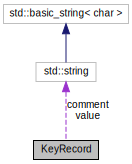
\includegraphics[width=204pt]{da/d5d/structKeyRecord__coll__graph}
\end{center}
\end{figure}
\subsection*{\-Public \-Member \-Functions}
\begin{DoxyCompactItemize}
\item 
\hypertarget{structKeyRecord_adb2df461920a68e399eb275601b4162d}{{\bfseries \-Key\-Record} (const string value)}\label{dc/dfa/structKeyRecord_adb2df461920a68e399eb275601b4162d}

\item 
\hypertarget{structKeyRecord_adf859a9e00ca7a1f5b217d0b498e22fe}{{\bfseries \-Key\-Record} (const string, const string, int)}\label{dc/dfa/structKeyRecord_adf859a9e00ca7a1f5b217d0b498e22fe}

\item 
\hypertarget{structKeyRecord_a8ae401ed4c0eff987d128b35087d96a1}{void {\bfseries set\-Value} (const string)}\label{dc/dfa/structKeyRecord_a8ae401ed4c0eff987d128b35087d96a1}

\item 
\hypertarget{structKeyRecord_a63587c62d362bfc8daa56aeec9d4c4f8}{void {\bfseries set\-Comment} (string)}\label{dc/dfa/structKeyRecord_a63587c62d362bfc8daa56aeec9d4c4f8}

\item 
\hypertarget{structKeyRecord_adee7f01f8d7b854a3ee122b3e949c8c2}{void {\bfseries set\-Pos\-Ptr} (int)}\label{dc/dfa/structKeyRecord_adee7f01f8d7b854a3ee122b3e949c8c2}

\item 
\hypertarget{structKeyRecord_a6d7e9380759ddb6f1acf7f5f8e10d740}{string \& {\bfseries get\-Value} ()}\label{dc/dfa/structKeyRecord_a6d7e9380759ddb6f1acf7f5f8e10d740}

\item 
\hypertarget{structKeyRecord_aa60c71d2a54153e4cff53b415cc4a110}{string \& {\bfseries get\-Comment} ()}\label{dc/dfa/structKeyRecord_aa60c71d2a54153e4cff53b415cc4a110}

\item 
\hypertarget{structKeyRecord_a90bf6993ecf929f2e9c4d6e388708c50}{int {\bfseries get\-Pos\-Ptr} ()}\label{dc/dfa/structKeyRecord_a90bf6993ecf929f2e9c4d6e388708c50}

\item 
\hypertarget{structKeyRecord_aeb4414945e397b7e8be240a96fa99723}{string {\bfseries operator()} (const \hyperlink{structKeyRecord}{\-Key\-Record} \&record)}\label{dc/dfa/structKeyRecord_aeb4414945e397b7e8be240a96fa99723}

\end{DoxyCompactItemize}
\subsection*{\-Protected \-Attributes}
\begin{DoxyCompactItemize}
\item 
\hypertarget{structKeyRecord_a81186e6db91374fc07fffb11b696ae7f}{string {\bfseries value}}\label{dc/dfa/structKeyRecord_a81186e6db91374fc07fffb11b696ae7f}

\item 
\hypertarget{structKeyRecord_aaa62600eaa986e1bb53f98e4aeebbfb9}{string {\bfseries comment}}\label{dc/dfa/structKeyRecord_aaa62600eaa986e1bb53f98e4aeebbfb9}

\item 
\hypertarget{structKeyRecord_af845a4d162b333f94cd8c81a067a65bb}{int {\bfseries \-Pos\-Ptr}}\label{dc/dfa/structKeyRecord_af845a4d162b333f94cd8c81a067a65bb}

\end{DoxyCompactItemize}


\-The documentation for this struct was generated from the following files\-:\begin{DoxyCompactItemize}
\item 
include/\hyperlink{iniReader_8h}{ini\-Reader.\-h}\item 
src/ini\-Reader.\-cpp\end{DoxyCompactItemize}

\hypertarget{structroundRobinInfo}{\section{round\-Robin\-Info \-Struct \-Reference}
\label{d2/de3/structroundRobinInfo}\index{round\-Robin\-Info@{round\-Robin\-Info}}
}


\-Struct containing process info specific for \-Round-\/\-Robin scheduling.  




{\ttfamily \#include $<$round\-\_\-robin.\-h$>$}

\subsection*{\-Public \-Attributes}
\begin{DoxyCompactItemize}
\item 
\hypertarget{structroundRobinInfo_a6c27850c4a7950e4aaa7cbcd532dca4b}{unsigned int \hyperlink{structroundRobinInfo_a6c27850c4a7950e4aaa7cbcd532dca4b}{blocked\-Index}}\label{d2/de3/structroundRobinInfo_a6c27850c4a7950e4aaa7cbcd532dca4b}

\begin{DoxyCompactList}\small\item\em \-Index position in blocked vector. \end{DoxyCompactList}\end{DoxyCompactItemize}


\-The documentation for this struct was generated from the following file\-:\begin{DoxyCompactItemize}
\item 
include/scheduler/\hyperlink{round__robin_8h}{round\-\_\-robin.\-h}\end{DoxyCompactItemize}

\hypertarget{structsCmdOptions}{\section{s\-Cmd\-Options \-Struct \-Reference}
\label{d2/db8/structsCmdOptions}\index{s\-Cmd\-Options@{s\-Cmd\-Options}}
}


\-All the settings files, traces and setting overrides from command line.  




{\ttfamily \#include $<$data\-\_\-structs.\-h$>$}



\-Collaboration diagram for s\-Cmd\-Options\-:\nopagebreak
\begin{figure}[H]
\begin{center}
\leavevmode
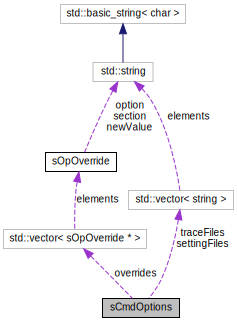
\includegraphics[width=309pt]{d0/de9/structsCmdOptions__coll__graph}
\end{center}
\end{figure}
\subsection*{\-Public \-Attributes}
\begin{DoxyCompactItemize}
\item 
\hypertarget{structsCmdOptions_afba8ae78df0568781a69f72476f36805}{vector$<$ string $>$ {\bfseries setting\-Files}}\label{d2/db8/structsCmdOptions_afba8ae78df0568781a69f72476f36805}

\item 
\hypertarget{structsCmdOptions_ada3acf44b12be001579ba43f6cd639bf}{vector$<$ string $>$ {\bfseries trace\-Files}}\label{d2/db8/structsCmdOptions_ada3acf44b12be001579ba43f6cd639bf}

\item 
\hypertarget{structsCmdOptions_a54e24cd92212dbee24e8a62d3802bdc8}{vector$<$ \hyperlink{structsOpOverride}{s\-Op\-Override} $\ast$ $>$ {\bfseries overrides}}\label{d2/db8/structsCmdOptions_a54e24cd92212dbee24e8a62d3802bdc8}

\end{DoxyCompactItemize}


\-The documentation for this struct was generated from the following file\-:\begin{DoxyCompactItemize}
\item 
include/\hyperlink{data__structs_8h}{data\-\_\-structs.\-h}\end{DoxyCompactItemize}

\hypertarget{structsIOContext}{\section{s\-I\-O\-Context \-Struct \-Reference}
\label{de/d05/structsIOContext}\index{s\-I\-O\-Context@{s\-I\-O\-Context}}
}


\-Struct for holding the context of an \-I/\-O operation.  




{\ttfamily \#include $<$io\-\_\-control.\-h$>$}



\-Collaboration diagram for s\-I\-O\-Context\-:\nopagebreak
\begin{figure}[H]
\begin{center}
\leavevmode
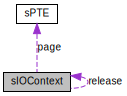
\includegraphics[width=199pt]{da/d83/structsIOContext__coll__graph}
\end{center}
\end{figure}
\subsection*{\-Public \-Attributes}
\begin{DoxyCompactItemize}
\item 
\hypertarget{structsIOContext_a59c80b76f45173eb0aa17c873f962910}{uint32\-\_\-t \hyperlink{structsIOContext_a59c80b76f45173eb0aa17c873f962910}{pid}}\label{de/d05/structsIOContext_a59c80b76f45173eb0aa17c873f962910}

\begin{DoxyCompactList}\small\item\em \-P\-I\-D of process that this \-I/\-O is for. \end{DoxyCompactList}\item 
\hypertarget{structsIOContext_af810e0e396ab38bc4388c250be40842e}{\hyperlink{structsPTE}{s\-P\-T\-E} $\ast$ \hyperlink{structsIOContext_af810e0e396ab38bc4388c250be40842e}{page}}\label{de/d05/structsIOContext_af810e0e396ab38bc4388c250be40842e}

\begin{DoxyCompactList}\small\item\em \-Page that is being either moved in or out. \end{DoxyCompactList}\item 
\hypertarget{structsIOContext_a71797bca2d785faa773940c5e16f84ed}{int \hyperlink{structsIOContext_a71797bca2d785faa773940c5e16f84ed}{time}}\label{de/d05/structsIOContext_a71797bca2d785faa773940c5e16f84ed}

\begin{DoxyCompactList}\small\item\em \-Time remaining on this \-I/\-O. \end{DoxyCompactList}\item 
\hypertarget{structsIOContext_ab832d28a1251bc233e5e5cf682622c08}{\hyperlink{structsIOContext}{s\-I\-O\-Context} $\ast$ \hyperlink{structsIOContext_ab832d28a1251bc233e5e5cf682622c08}{release}}\label{de/d05/structsIOContext_ab832d28a1251bc233e5e5cf682622c08}

\begin{DoxyCompactList}\small\item\em \-Release this waiting \-I/\-O when this one finishes. \end{DoxyCompactList}\end{DoxyCompactItemize}


\subsection{\-Detailed \-Description}


\-The documentation for this struct was generated from the following file\-:\begin{DoxyCompactItemize}
\item 
include/io\-\_\-control.\-h\end{DoxyCompactItemize}

\hypertarget{structsOpOverride}{\section{s\-Op\-Override \-Struct \-Reference}
\label{d2/d28/structsOpOverride}\index{s\-Op\-Override@{s\-Op\-Override}}
}


\-Struct for holding a settings overrides from command line.  




{\ttfamily \#include $<$data\-\_\-structs.\-h$>$}



\-Collaboration diagram for s\-Op\-Override\-:\nopagebreak
\begin{figure}[H]
\begin{center}
\leavevmode
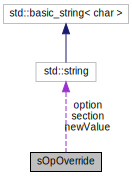
\includegraphics[width=204pt]{d5/d1e/structsOpOverride__coll__graph}
\end{center}
\end{figure}
\subsection*{\-Public \-Attributes}
\begin{DoxyCompactItemize}
\item 
\hypertarget{structsOpOverride_a4620283115615d0c3d5e7cd1050e2594}{string {\bfseries section}}\label{d2/d28/structsOpOverride_a4620283115615d0c3d5e7cd1050e2594}

\item 
\hypertarget{structsOpOverride_a07eef5f58cccc720b8779df250674ae2}{string {\bfseries option}}\label{d2/d28/structsOpOverride_a07eef5f58cccc720b8779df250674ae2}

\item 
\hypertarget{structsOpOverride_ad318da346965eb8ec241f744690f6db8}{string {\bfseries new\-Value}}\label{d2/d28/structsOpOverride_ad318da346965eb8ec241f744690f6db8}

\end{DoxyCompactItemize}


\-The documentation for this struct was generated from the following file\-:\begin{DoxyCompactItemize}
\item 
include/\hyperlink{data__structs_8h}{data\-\_\-structs.\-h}\end{DoxyCompactItemize}

\hypertarget{structsProc}{\section{s\-Proc \-Struct \-Reference}
\label{d4/d8e/structsProc}\index{s\-Proc@{s\-Proc}}
}


\-Struct representing a process.  




{\ttfamily \#include $<$data\-\_\-structs.\-h$>$}



\-Collaboration diagram for s\-Proc\-:\nopagebreak
\begin{figure}[H]
\begin{center}
\leavevmode
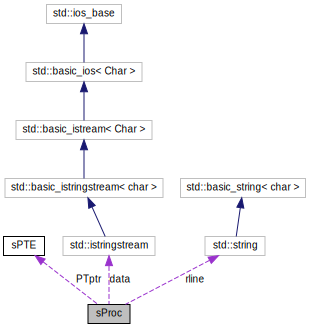
\includegraphics[width=350pt]{df/dc9/structsProc__coll__graph}
\end{center}
\end{figure}
\subsection*{\-Public \-Attributes}
\begin{DoxyCompactItemize}
\item 
\hypertarget{structsProc_acba0c89d09f7973a240a9b229a31fabe}{unsigned int \hyperlink{structsProc_acba0c89d09f7973a240a9b229a31fabe}{pid}}\label{d4/d8e/structsProc_acba0c89d09f7973a240a9b229a31fabe}

\begin{DoxyCompactList}\small\item\em \-Process \-P\-I\-D. \end{DoxyCompactList}\item 
\hypertarget{structsProc_a621d8ad464b51d3cbf0ccd54ee3853bd}{uint16\-\_\-t \hyperlink{structsProc_a621d8ad464b51d3cbf0ccd54ee3853bd}{cswitches}}\label{d4/d8e/structsProc_a621d8ad464b51d3cbf0ccd54ee3853bd}

\begin{DoxyCompactList}\small\item\em \# of \-Context \-Switches \end{DoxyCompactList}\item 
\hypertarget{structsProc_a9a31e35852f9c3f517e2a685d919767f}{int {\bfseries page\-Faults}}\label{d4/d8e/structsProc_a9a31e35852f9c3f517e2a685d919767f}

\item 
\hypertarget{structsProc_a80729551ba1fa1d96a31114efbe51ebd}{int {\bfseries tlbhit}}\label{d4/d8e/structsProc_a80729551ba1fa1d96a31114efbe51ebd}

\item 
\hypertarget{structsProc_addf3df48be9557e0adfa8714cdf2549c}{int {\bfseries tlbmiss}}\label{d4/d8e/structsProc_addf3df48be9557e0adfa8714cdf2549c}

\item 
\hypertarget{structsProc_a5b9e75f676b6cf3b034c6bb64e1221e0}{int \hyperlink{structsProc_a5b9e75f676b6cf3b034c6bb64e1221e0}{clock\-Time}}\label{d4/d8e/structsProc_a5b9e75f676b6cf3b034c6bb64e1221e0}

\begin{DoxyCompactList}\small\item\em \-Time spent executing. \end{DoxyCompactList}\item 
\hypertarget{structsProc_a9079bdad478d80b701669442a8919f94}{int \hyperlink{structsProc_a9079bdad478d80b701669442a8919f94}{finish\-Time}}\label{d4/d8e/structsProc_a9079bdad478d80b701669442a8919f94}

\begin{DoxyCompactList}\small\item\em \-V\-C when process finished. \end{DoxyCompactList}\item 
\hypertarget{structsProc_adc5c77141ef1d0ce31aef263f5085871}{istringstream $\ast$ \hyperlink{structsProc_adc5c77141ef1d0ce31aef263f5085871}{data}}\label{d4/d8e/structsProc_adc5c77141ef1d0ce31aef263f5085871}

\begin{DoxyCompactList}\small\item\em \-Text data of process. \end{DoxyCompactList}\item 
\hypertarget{structsProc_a1c3a52cf9c8388b00fddeff11faec8ed}{int \hyperlink{structsProc_a1c3a52cf9c8388b00fddeff11faec8ed}{\-P\-C}}\label{d4/d8e/structsProc_a1c3a52cf9c8388b00fddeff11faec8ed}

\begin{DoxyCompactList}\small\item\em \-Program \-Counter. \end{DoxyCompactList}\item 
int \hyperlink{structsProc_a915cc193d810601697481767854a9b05}{max\-P\-C}
\begin{DoxyCompactList}\small\item\em \-Max \-P\-C. \end{DoxyCompactList}\item 
\hypertarget{structsProc_af4083409a9efd6e6eeafcf918e72423d}{bool \hyperlink{structsProc_af4083409a9efd6e6eeafcf918e72423d}{restart}}\label{d4/d8e/structsProc_af4083409a9efd6e6eeafcf918e72423d}

\begin{DoxyCompactList}\small\item\em \-Used to flag an instruction restart. \end{DoxyCompactList}\item 
\hypertarget{structsProc_af173141c3ed2ea7cfa2fb571e7c8a52a}{bool \hyperlink{structsProc_af173141c3ed2ea7cfa2fb571e7c8a52a}{circular\-Fault\-Check}}\label{d4/d8e/structsProc_af173141c3ed2ea7cfa2fb571e7c8a52a}

\begin{DoxyCompactList}\small\item\em \-If the same process faults on the same instruction more than once the cpu notifies the core. \end{DoxyCompactList}\item 
\hypertarget{structsProc_a82699971a08c9889bb70cdb000c2a65a}{string \hyperlink{structsProc_a82699971a08c9889bb70cdb000c2a65a}{rline}}\label{d4/d8e/structsProc_a82699971a08c9889bb70cdb000c2a65a}

\begin{DoxyCompactList}\small\item\em \-Process instruction for the restart. \end{DoxyCompactList}\item 
\hypertarget{structsProc_a469832c44beab71535219bc020956dcd}{\hyperlink{structsPTE}{s\-P\-T\-E} $\ast$ \hyperlink{structsProc_a469832c44beab71535219bc020956dcd}{\-P\-Tptr}}\label{d4/d8e/structsProc_a469832c44beab71535219bc020956dcd}

\begin{DoxyCompactList}\small\item\em \-Pointer to process' page table. \end{DoxyCompactList}\item 
void $\ast$ \hyperlink{structsProc_ab2e14e8d2e13b2d661c81e25d7bb2b2c}{schedule\-Data}
\begin{DoxyCompactList}\small\item\em \-Scheduler specific data. \end{DoxyCompactList}\end{DoxyCompactItemize}


\subsection{\-Member \-Data \-Documentation}
\hypertarget{structsProc_a915cc193d810601697481767854a9b05}{\index{s\-Proc@{s\-Proc}!max\-P\-C@{max\-P\-C}}
\index{max\-P\-C@{max\-P\-C}!sProc@{s\-Proc}}
\subsubsection[{max\-P\-C}]{\setlength{\rightskip}{0pt plus 5cm}int {\bf s\-Proc\-::max\-P\-C}}}\label{d4/d8e/structsProc_a915cc193d810601697481767854a9b05}
\-Based on size of process file 

\-Referenced by c\-V\-M\-M\-::cleanup\-Process(), and c\-C\-P\-U\-::run().

\hypertarget{structsProc_ab2e14e8d2e13b2d661c81e25d7bb2b2c}{\index{s\-Proc@{s\-Proc}!schedule\-Data@{schedule\-Data}}
\index{schedule\-Data@{schedule\-Data}!sProc@{s\-Proc}}
\subsubsection[{schedule\-Data}]{\setlength{\rightskip}{0pt plus 5cm}void$\ast$ {\bf s\-Proc\-::schedule\-Data}}}\label{d4/d8e/structsProc_ab2e14e8d2e13b2d661c81e25d7bb2b2c}
\-Always round robin for this project 

\-The documentation for this struct was generated from the following file\-:\begin{DoxyCompactItemize}
\item 
include/\hyperlink{data__structs_8h}{data\-\_\-structs.\-h}\end{DoxyCompactItemize}

\hypertarget{structsPTE}{\section{s\-P\-T\-E \-Struct \-Reference}
\label{db/d4b/structsPTE}\index{s\-P\-T\-E@{s\-P\-T\-E}}
}


\-A struct representing a single page table entry.  




{\ttfamily \#include $<$data\-\_\-structs.\-h$>$}

\subsection*{\-Public \-Attributes}
\begin{DoxyCompactItemize}
\item 
\hypertarget{structsPTE_a7f83c711e07dc476cceb9ac15ea010d7}{uint32\-\_\-t \hyperlink{structsPTE_a7f83c711e07dc476cceb9ac15ea010d7}{frame}}\label{db/d4b/structsPTE_a7f83c711e07dc476cceb9ac15ea010d7}

\begin{DoxyCompactList}\small\item\em \-Frame that this \-P\-T\-E maps to. \end{DoxyCompactList}\item 
\hypertarget{structsPTE_a8b5b24029a238d20968676a78a81928c}{int \hyperlink{structsPTE_a8b5b24029a238d20968676a78a81928c}{timestamp}}\label{db/d4b/structsPTE_a8b5b24029a238d20968676a78a81928c}

\begin{DoxyCompactList}\small\item\em \-This gets set in hardware by the \-M\-M\-U. \end{DoxyCompactList}\item 
bool \hyperlink{structsPTE_a5088ab9c05c286c643ef97d04a3c9dad}{flags} \mbox{[}3\mbox{]}
\begin{DoxyCompactList}\small\item\em \-Page \-Table \-Entry (\-P\-T\-E) \-V\-M flags. \end{DoxyCompactList}\item 
\hypertarget{structsPTE_a73f0dd13e3c1909cee215ff78c99e487}{uint8\-\_\-t \hyperlink{structsPTE_a73f0dd13e3c1909cee215ff78c99e487}{time}}\label{db/d4b/structsPTE_a73f0dd13e3c1909cee215ff78c99e487}

\begin{DoxyCompactList}\small\item\em \-This is set in software by the pr\-\_\-lru\-Approx after each quanta or on a page fault. \end{DoxyCompactList}\end{DoxyCompactItemize}


\subsection{\-Member \-Data \-Documentation}
\hypertarget{structsPTE_a5088ab9c05c286c643ef97d04a3c9dad}{\index{s\-P\-T\-E@{s\-P\-T\-E}!flags@{flags}}
\index{flags@{flags}!sPTE@{s\-P\-T\-E}}
\subsubsection[{flags}]{\setlength{\rightskip}{0pt plus 5cm}bool {\bf s\-P\-T\-E\-::flags}\mbox{[}3\mbox{]}}}\label{db/d4b/structsPTE_a5088ab9c05c286c643ef97d04a3c9dad}
flags\mbox{[}0\mbox{]}\-: \-Present/absent flags\mbox{[}1\mbox{]}\-: \-Dirty flags\mbox{[}2\mbox{]}\-: \-Referenced 

\-Referenced by c\-M\-M\-U\-::add\-T\-L\-B(), c\-V\-M\-M\-::cleanup\-Process(), c\-P\-R\-Fifo\-::clear\-Pages(), c\-P\-R\-Lru\-Approx\-::clear\-Pages(), c\-P\-R\-Lru\-::clear\-Pages(), c\-M\-M\-U\-::flush\-T\-L\-B(), c\-P\-R\-Fifo\-::resolve\-Page\-Fault(), c\-P\-R\-Lru\-Approx\-::resolve\-Page\-Fault(), c\-P\-R\-Lru\-::resolve\-Page\-Fault(), c\-M\-M\-U\-::sync\-T\-L\-B(), c\-I\-O\-Control\-::tick(), and c\-P\-R\-Lru\-Approx\-::update\-Time().



\-The documentation for this struct was generated from the following file\-:\begin{DoxyCompactItemize}
\item 
include/\hyperlink{data__structs_8h}{data\-\_\-structs.\-h}\end{DoxyCompactItemize}

\hypertarget{structsPTEOwner}{\section{s\-P\-T\-E\-Owner \-Struct \-Reference}
\label{d2/d96/structsPTEOwner}\index{s\-P\-T\-E\-Owner@{s\-P\-T\-E\-Owner}}
}


\-A struct used to associate a process with a particular page.  




{\ttfamily \#include $<$data\-\_\-structs.\-h$>$}



\-Collaboration diagram for s\-P\-T\-E\-Owner\-:\nopagebreak
\begin{figure}[H]
\begin{center}
\leavevmode
\includegraphics[width=150pt]{db/d9a/structsPTEOwner__coll__graph}
\end{center}
\end{figure}
\subsection*{\-Public \-Attributes}
\begin{DoxyCompactItemize}
\item 
\hypertarget{structsPTEOwner_a744b2c55b104fba03ec7c1f52f5fc49c}{uint32\-\_\-t {\bfseries pid}}\label{d2/d96/structsPTEOwner_a744b2c55b104fba03ec7c1f52f5fc49c}

\item 
\hypertarget{structsPTEOwner_ac0f7424fdfa9488652bfb14cdbb9eb89}{\hyperlink{structsPTE}{s\-P\-T\-E} $\ast$ {\bfseries page}}\label{d2/d96/structsPTEOwner_ac0f7424fdfa9488652bfb14cdbb9eb89}

\end{DoxyCompactItemize}


\subsection{\-Detailed \-Description}


\-The documentation for this struct was generated from the following file\-:\begin{DoxyCompactItemize}
\item 
include/\hyperlink{data__structs_8h}{data\-\_\-structs.\-h}\end{DoxyCompactItemize}

\hypertarget{structsTLBE}{\section{s\-T\-L\-B\-E \-Struct \-Reference}
\label{d2/deb/structsTLBE}\index{s\-T\-L\-B\-E@{s\-T\-L\-B\-E}}
}


\-Struct representing a single entry in the \-T\-L\-B.  




{\ttfamily \#include $<$mmu.\-h$>$}

\subsection*{\-Public \-Attributes}
\begin{DoxyCompactItemize}
\item 
\hypertarget{structsTLBE_a4010857b71377706a604c279ace18d01}{uint32\-\_\-t {\bfseries \-V\-P\-N}}\label{d2/deb/structsTLBE_a4010857b71377706a604c279ace18d01}

\item 
\hypertarget{structsTLBE_a4b59c05e37a16e8cae375f4196035c70}{uint32\-\_\-t {\bfseries frame}}\label{d2/deb/structsTLBE_a4b59c05e37a16e8cae375f4196035c70}

\item 
\hypertarget{structsTLBE_a1f482585fac2299e1c083bef6a5391ef}{int {\bfseries timestamp}}\label{d2/deb/structsTLBE_a1f482585fac2299e1c083bef6a5391ef}

\item 
bool \hyperlink{structsTLBE_a49cd068c40f5bb2698fb351d4356492e}{valid}
\begin{DoxyCompactList}\small\item\em \-Is this a valid translation? \end{DoxyCompactList}\item 
\hypertarget{structsTLBE_a9b13016950c8670388e23d5a818d3c53}{bool {\bfseries dirty}}\label{d2/deb/structsTLBE_a9b13016950c8670388e23d5a818d3c53}

\item 
\hypertarget{structsTLBE_a3d9f86a07a5cadff19239a7eaf713e71}{bool {\bfseries ref}}\label{d2/deb/structsTLBE_a3d9f86a07a5cadff19239a7eaf713e71}

\end{DoxyCompactItemize}


\subsection{\-Member \-Data \-Documentation}
\hypertarget{structsTLBE_a49cd068c40f5bb2698fb351d4356492e}{\index{s\-T\-L\-B\-E@{s\-T\-L\-B\-E}!valid@{valid}}
\index{valid@{valid}!sTLBE@{s\-T\-L\-B\-E}}
\subsubsection[{valid}]{\setlength{\rightskip}{0pt plus 5cm}bool {\bf s\-T\-L\-B\-E\-::valid}}}\label{d2/deb/structsTLBE_a49cd068c40f5bb2698fb351d4356492e}
\-If false, the \-M\-M\-U will ignore any cache hits on this entry. \-This is also used in flushing the tlb. 

\-Referenced by c\-M\-M\-U\-::add\-T\-L\-B(), and c\-M\-M\-U\-::flush\-T\-L\-B().



\-The documentation for this struct was generated from the following file\-:\begin{DoxyCompactItemize}
\item 
include/\hyperlink{mmu_8h}{mmu.\-h}\end{DoxyCompactItemize}

\chapter{\-File \-Documentation}
\hypertarget{cpu_8h}{\section{include/cpu.h \-File \-Reference}
\label{dc/da7/cpu_8h}\index{include/cpu.\-h@{include/cpu.\-h}}
}
{\ttfamily \#include \char`\"{}mmu.\-h\char`\"{}}\*
{\ttfamily \#include \char`\"{}data\-\_\-structs.\-h\char`\"{}}\*
{\ttfamily \#include \char`\"{}ini\-Reader.\-h\char`\"{}}\*
{\ttfamily \#include \char`\"{}utility/logger.\-h\char`\"{}}\*
{\ttfamily \#include \char`\"{}vmm\-\_\-core.\-h\char`\"{}}\*
\-Include dependency graph for cpu.\-h\-:\nopagebreak
\begin{figure}[H]
\begin{center}
\leavevmode
\includegraphics[width=350pt]{d4/d37/cpu_8h__incl}
\end{center}
\end{figure}
\-This graph shows which files directly or indirectly include this file\-:\nopagebreak
\begin{figure}[H]
\begin{center}
\leavevmode
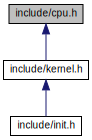
\includegraphics[width=350pt]{d8/de6/cpu_8h__dep__incl}
\end{center}
\end{figure}
\subsection*{\-Classes}
\begin{DoxyCompactItemize}
\item 
class \hyperlink{classcCPU}{c\-C\-P\-U}
\begin{DoxyCompactList}\small\item\em \-Very \-Simple \-C\-P\-U. \end{DoxyCompactList}\end{DoxyCompactItemize}
\subsection*{\-Enumerations}
\begin{DoxyCompactItemize}
\item 
enum \hyperlink{cpu_8h_a79dd30df748ae6e82b07d59888cbf05a}{e\-C\-P\-U\-State} \{ \*
\hyperlink{cpu_8h_a79dd30df748ae6e82b07d59888cbf05aaa252df7bb52b9092b5a403bd773c4ab7}{\-C\-P\-U\-\_\-\-O\-K} =  0x1, 
\hyperlink{cpu_8h_a79dd30df748ae6e82b07d59888cbf05aaae42c2aa12e3045e16b4170ce1985369}{\-C\-P\-U\-\_\-\-P\-F} =  \-C\-P\-U\-\_\-\-O\-K $<$$<$ 1, 
\hyperlink{cpu_8h_a79dd30df748ae6e82b07d59888cbf05aa358293772016df0374d4a3760e45c4f2}{\-C\-P\-U\-\_\-\-T\-E\-R\-M} =  \-C\-P\-U\-\_\-\-P\-F $<$$<$ 1, 
\hyperlink{cpu_8h_a79dd30df748ae6e82b07d59888cbf05aa254be8e08491090445866214398e163c}{\-C\-P\-U\-\_\-\-E\-X} =  \-C\-P\-U\-\_\-\-T\-E\-R\-M $<$$<$ 1, 
\*
\hyperlink{cpu_8h_a79dd30df748ae6e82b07d59888cbf05aa5fd7a8485d51f46b6dc88dba870c2e65}{\-C\-P\-U\-\_\-\-C\-I\-R\-C\-\_\-\-P\-F} =  \-C\-P\-U\-\_\-\-E\-X $<$$<$ 1
 \}
\begin{DoxyCompactList}\small\item\em \-Status of the execution quantum termination. \end{DoxyCompactList}\end{DoxyCompactItemize}


\subsection{\-Detailed \-Description}


\subsection{\-Enumeration \-Type \-Documentation}
\hypertarget{cpu_8h_a79dd30df748ae6e82b07d59888cbf05a}{\index{cpu.\-h@{cpu.\-h}!e\-C\-P\-U\-State@{e\-C\-P\-U\-State}}
\index{e\-C\-P\-U\-State@{e\-C\-P\-U\-State}!cpu.h@{cpu.\-h}}
\subsubsection[{e\-C\-P\-U\-State}]{\setlength{\rightskip}{0pt plus 5cm}enum {\bf e\-C\-P\-U\-State}}}\label{dc/da7/cpu_8h_a79dd30df748ae6e82b07d59888cbf05a}
\begin{Desc}
\item[\-Enumerator\-: ]\par
\begin{description}
\index{\-C\-P\-U\-\_\-\-O\-K@{\-C\-P\-U\-\_\-\-O\-K}!cpu.\-h@{cpu.\-h}}\index{cpu.\-h@{cpu.\-h}!\-C\-P\-U\-\_\-\-O\-K@{\-C\-P\-U\-\_\-\-O\-K}}\item[{\em 
\hypertarget{cpu_8h_a79dd30df748ae6e82b07d59888cbf05aaa252df7bb52b9092b5a403bd773c4ab7}{\-C\-P\-U\-\_\-\-O\-K}\label{dc/da7/cpu_8h_a79dd30df748ae6e82b07d59888cbf05aaa252df7bb52b9092b5a403bd773c4ab7}
}]\-C\-P\-U finished executing instruction ok. \index{\-C\-P\-U\-\_\-\-P\-F@{\-C\-P\-U\-\_\-\-P\-F}!cpu.\-h@{cpu.\-h}}\index{cpu.\-h@{cpu.\-h}!\-C\-P\-U\-\_\-\-P\-F@{\-C\-P\-U\-\_\-\-P\-F}}\item[{\em 
\hypertarget{cpu_8h_a79dd30df748ae6e82b07d59888cbf05aaae42c2aa12e3045e16b4170ce1985369}{\-C\-P\-U\-\_\-\-P\-F}\label{dc/da7/cpu_8h_a79dd30df748ae6e82b07d59888cbf05aaae42c2aa12e3045e16b4170ce1985369}
}]\-C\-P\-U/\-M\-M\-U incured a page fault. \index{\-C\-P\-U\-\_\-\-T\-E\-R\-M@{\-C\-P\-U\-\_\-\-T\-E\-R\-M}!cpu.\-h@{cpu.\-h}}\index{cpu.\-h@{cpu.\-h}!\-C\-P\-U\-\_\-\-T\-E\-R\-M@{\-C\-P\-U\-\_\-\-T\-E\-R\-M}}\item[{\em 
\hypertarget{cpu_8h_a79dd30df748ae6e82b07d59888cbf05aa358293772016df0374d4a3760e45c4f2}{\-C\-P\-U\-\_\-\-T\-E\-R\-M}\label{dc/da7/cpu_8h_a79dd30df748ae6e82b07d59888cbf05aa358293772016df0374d4a3760e45c4f2}
}]\-Process execution termination. \index{\-C\-P\-U\-\_\-\-E\-X@{\-C\-P\-U\-\_\-\-E\-X}!cpu.\-h@{cpu.\-h}}\index{cpu.\-h@{cpu.\-h}!\-C\-P\-U\-\_\-\-E\-X@{\-C\-P\-U\-\_\-\-E\-X}}\item[{\em 
\hypertarget{cpu_8h_a79dd30df748ae6e82b07d59888cbf05aa254be8e08491090445866214398e163c}{\-C\-P\-U\-\_\-\-E\-X}\label{dc/da7/cpu_8h_a79dd30df748ae6e82b07d59888cbf05aa254be8e08491090445866214398e163c}
}]\-Process exception. \index{\-C\-P\-U\-\_\-\-C\-I\-R\-C\-\_\-\-P\-F@{\-C\-P\-U\-\_\-\-C\-I\-R\-C\-\_\-\-P\-F}!cpu.\-h@{cpu.\-h}}\index{cpu.\-h@{cpu.\-h}!\-C\-P\-U\-\_\-\-C\-I\-R\-C\-\_\-\-P\-F@{\-C\-P\-U\-\_\-\-C\-I\-R\-C\-\_\-\-P\-F}}\item[{\em 
\hypertarget{cpu_8h_a79dd30df748ae6e82b07d59888cbf05aa5fd7a8485d51f46b6dc88dba870c2e65}{\-C\-P\-U\-\_\-\-C\-I\-R\-C\-\_\-\-P\-F}\label{dc/da7/cpu_8h_a79dd30df748ae6e82b07d59888cbf05aa5fd7a8485d51f46b6dc88dba870c2e65}
}]\-Potential circular page fault detected by cpu. \end{description}
\end{Desc}


\hypertarget{data__structs_8h}{\section{include/data\-\_\-structs.h \-File \-Reference}
\label{d5/dee/data__structs_8h}\index{include/data\-\_\-structs.\-h@{include/data\-\_\-structs.\-h}}
}
{\ttfamily \#include $<$vector$>$}\*
{\ttfamily \#include $<$string$>$}\*
{\ttfamily \#include $<$sstream$>$}\*
{\ttfamily \#include $<$iostream$>$}\*
{\ttfamily \#include $<$inttypes.\-h$>$}\*
\-Include dependency graph for data\-\_\-structs.\-h\-:\nopagebreak
\begin{figure}[H]
\begin{center}
\leavevmode
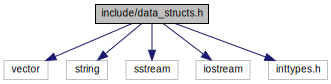
\includegraphics[width=350pt]{da/dd6/data__structs_8h__incl}
\end{center}
\end{figure}
\-This graph shows which files directly or indirectly include this file\-:\nopagebreak
\begin{figure}[H]
\begin{center}
\leavevmode
\includegraphics[width=350pt]{d1/dc3/data__structs_8h__dep__incl}
\end{center}
\end{figure}
\subsection*{\-Classes}
\begin{DoxyCompactItemize}
\item 
struct \hyperlink{structsPTE}{s\-P\-T\-E}
\begin{DoxyCompactList}\small\item\em \-A struct representing a single page table entry. \end{DoxyCompactList}\item 
struct \hyperlink{structsPTEOwner}{s\-P\-T\-E\-Owner}
\begin{DoxyCompactList}\small\item\em \-A struct used to associate a process with a particular page. \end{DoxyCompactList}\item 
struct \hyperlink{structsProc}{s\-Proc}
\begin{DoxyCompactList}\small\item\em \-Struct representing a process. \end{DoxyCompactList}\item 
struct \hyperlink{structsOpOverride}{s\-Op\-Override}
\begin{DoxyCompactList}\small\item\em \-Struct for holding a settings overrides from command line. \end{DoxyCompactList}\item 
struct \hyperlink{structsCmdOptions}{s\-Cmd\-Options}
\begin{DoxyCompactList}\small\item\em \-All the settings files, traces and setting overrides from command line. \end{DoxyCompactList}\end{DoxyCompactItemize}
\subsection*{\-Enumerations}
\begin{DoxyCompactItemize}
\item 
enum \hyperlink{data__structs_8h_a35b22dfd92090451943b80c7c0c896e5}{e\-Flag\-Index} \{ \hyperlink{data__structs_8h_a35b22dfd92090451943b80c7c0c896e5a0946ef97ddb136799838a467d2f51e50}{\-F\-I\-\_\-\-P\-R\-E\-S\-E\-N\-T}, 
\hyperlink{data__structs_8h_a35b22dfd92090451943b80c7c0c896e5a3de6e98e4678bda91123c8ffc2ccfa20}{\-F\-I\-\_\-\-D\-I\-R\-T\-Y}, 
\hyperlink{data__structs_8h_a35b22dfd92090451943b80c7c0c896e5aeef98cde3e508a19470675b934520168}{\-F\-I\-\_\-\-R\-E\-F}
 \}
\begin{DoxyCompactList}\small\item\em \-Enum used for indexing \-P\-T\-E flags. \end{DoxyCompactList}\end{DoxyCompactItemize}


\subsection{\-Detailed \-Description}


\subsection{\-Enumeration \-Type \-Documentation}
\hypertarget{data__structs_8h_a35b22dfd92090451943b80c7c0c896e5}{\index{data\-\_\-structs.\-h@{data\-\_\-structs.\-h}!e\-Flag\-Index@{e\-Flag\-Index}}
\index{e\-Flag\-Index@{e\-Flag\-Index}!data_structs.h@{data\-\_\-structs.\-h}}
\subsubsection[{e\-Flag\-Index}]{\setlength{\rightskip}{0pt plus 5cm}enum {\bf e\-Flag\-Index}}}\label{d5/dee/data__structs_8h_a35b22dfd92090451943b80c7c0c896e5}
\begin{Desc}
\item[\-Enumerator\-: ]\par
\begin{description}
\index{\-F\-I\-\_\-\-P\-R\-E\-S\-E\-N\-T@{\-F\-I\-\_\-\-P\-R\-E\-S\-E\-N\-T}!data\-\_\-structs.\-h@{data\-\_\-structs.\-h}}\index{data\-\_\-structs.\-h@{data\-\_\-structs.\-h}!\-F\-I\-\_\-\-P\-R\-E\-S\-E\-N\-T@{\-F\-I\-\_\-\-P\-R\-E\-S\-E\-N\-T}}\item[{\em 
\hypertarget{data__structs_8h_a35b22dfd92090451943b80c7c0c896e5a0946ef97ddb136799838a467d2f51e50}{\-F\-I\-\_\-\-P\-R\-E\-S\-E\-N\-T}\label{d5/dee/data__structs_8h_a35b22dfd92090451943b80c7c0c896e5a0946ef97ddb136799838a467d2f51e50}
}]\-Access \-P\-T\-E present bit. \index{\-F\-I\-\_\-\-D\-I\-R\-T\-Y@{\-F\-I\-\_\-\-D\-I\-R\-T\-Y}!data\-\_\-structs.\-h@{data\-\_\-structs.\-h}}\index{data\-\_\-structs.\-h@{data\-\_\-structs.\-h}!\-F\-I\-\_\-\-D\-I\-R\-T\-Y@{\-F\-I\-\_\-\-D\-I\-R\-T\-Y}}\item[{\em 
\hypertarget{data__structs_8h_a35b22dfd92090451943b80c7c0c896e5a3de6e98e4678bda91123c8ffc2ccfa20}{\-F\-I\-\_\-\-D\-I\-R\-T\-Y}\label{d5/dee/data__structs_8h_a35b22dfd92090451943b80c7c0c896e5a3de6e98e4678bda91123c8ffc2ccfa20}
}]\-Access \-P\-T\-E dirty bit. \index{\-F\-I\-\_\-\-R\-E\-F@{\-F\-I\-\_\-\-R\-E\-F}!data\-\_\-structs.\-h@{data\-\_\-structs.\-h}}\index{data\-\_\-structs.\-h@{data\-\_\-structs.\-h}!\-F\-I\-\_\-\-R\-E\-F@{\-F\-I\-\_\-\-R\-E\-F}}\item[{\em 
\hypertarget{data__structs_8h_a35b22dfd92090451943b80c7c0c896e5aeef98cde3e508a19470675b934520168}{\-F\-I\-\_\-\-R\-E\-F}\label{d5/dee/data__structs_8h_a35b22dfd92090451943b80c7c0c896e5aeef98cde3e508a19470675b934520168}
}]\-Access \-P\-T\-E reference bit. \end{description}
\end{Desc}


\hypertarget{exceptions_8h}{\section{include/exceptions.h \-File \-Reference}
\label{d4/d03/exceptions_8h}\index{include/exceptions.\-h@{include/exceptions.\-h}}
}
\-This graph shows which files directly or indirectly include this file\-:\nopagebreak
\begin{figure}[H]
\begin{center}
\leavevmode
\includegraphics[width=350pt]{d5/d85/exceptions_8h__dep__incl}
\end{center}
\end{figure}
\subsection*{\-Classes}
\begin{DoxyCompactItemize}
\item 
class \hyperlink{classcException}{c\-Exception}
\begin{DoxyCompactList}\small\item\em \-Generic exception class. \end{DoxyCompactList}\item 
class \hyperlink{classcVMMExc}{c\-V\-M\-M\-Exc}
\begin{DoxyCompactList}\small\item\em \-A class handling exceptions in the \-V\-M\-M \-Core. \end{DoxyCompactList}\item 
class \hyperlink{classcIOExc}{c\-I\-O\-Exc}
\begin{DoxyCompactList}\small\item\em \-Class handling exceptions in the \-I/\-O system. \end{DoxyCompactList}\item 
class \hyperlink{classcPRExc}{c\-P\-R\-Exc}
\end{DoxyCompactItemize}
\subsection*{\-Enumerations}
\begin{DoxyCompactItemize}
\item 
enum \hyperlink{exceptions_8h_a5cf02777e008e49ed78b878634829334}{e\-Ex\-Type} \{ \hyperlink{exceptions_8h_a5cf02777e008e49ed78b878634829334a2f34e97dde992bdee53101787529483c}{\-P\-R\-\_\-\-N\-O\-\_\-\-F\-R\-A\-M\-E\-S\-\_\-\-A\-V\-A\-I\-L}
 \}
\begin{DoxyCompactList}\small\item\em \-Distinguish between exceptions in a generic class. \end{DoxyCompactList}\end{DoxyCompactItemize}


\subsection{\-Detailed \-Description}


\subsection{\-Enumeration \-Type \-Documentation}
\hypertarget{exceptions_8h_a5cf02777e008e49ed78b878634829334}{\index{exceptions.\-h@{exceptions.\-h}!e\-Ex\-Type@{e\-Ex\-Type}}
\index{e\-Ex\-Type@{e\-Ex\-Type}!exceptions.h@{exceptions.\-h}}
\subsubsection[{e\-Ex\-Type}]{\setlength{\rightskip}{0pt plus 5cm}enum {\bf e\-Ex\-Type}}}\label{d4/d03/exceptions_8h_a5cf02777e008e49ed78b878634829334}
\-Since we didn't really have time to expand the exception system for this project this never really expanded. \begin{Desc}
\item[\-Enumerator\-: ]\par
\begin{description}
\index{\-P\-R\-\_\-\-N\-O\-\_\-\-F\-R\-A\-M\-E\-S\-\_\-\-A\-V\-A\-I\-L@{\-P\-R\-\_\-\-N\-O\-\_\-\-F\-R\-A\-M\-E\-S\-\_\-\-A\-V\-A\-I\-L}!exceptions.\-h@{exceptions.\-h}}\index{exceptions.\-h@{exceptions.\-h}!\-P\-R\-\_\-\-N\-O\-\_\-\-F\-R\-A\-M\-E\-S\-\_\-\-A\-V\-A\-I\-L@{\-P\-R\-\_\-\-N\-O\-\_\-\-F\-R\-A\-M\-E\-S\-\_\-\-A\-V\-A\-I\-L}}\item[{\em 
\hypertarget{exceptions_8h_a5cf02777e008e49ed78b878634829334a2f34e97dde992bdee53101787529483c}{\-P\-R\-\_\-\-N\-O\-\_\-\-F\-R\-A\-M\-E\-S\-\_\-\-A\-V\-A\-I\-L}\label{d4/d03/exceptions_8h_a5cf02777e008e49ed78b878634829334a2f34e97dde992bdee53101787529483c}
}]\-No frames are available. \-Thrown by \-P\-R\-Module \end{description}
\end{Desc}


\hypertarget{iniReader_8h}{\section{include/ini\-Reader.h \-File \-Reference}
\label{d5/dfd/iniReader_8h}\index{include/ini\-Reader.\-h@{include/ini\-Reader.\-h}}
}
{\ttfamily \#include $<$stdlib.\-h$>$}\*
{\ttfamily \#include $<$string$>$}\*
{\ttfamily \#include $<$map$>$}\*
{\ttfamily \#include $<$vector$>$}\*
{\ttfamily \#include $<$iostream$>$}\*
{\ttfamily \#include $<$sstream$>$}\*
{\ttfamily \#include $<$fstream$>$}\*
\-Include dependency graph for ini\-Reader.\-h\-:\nopagebreak
\begin{figure}[H]
\begin{center}
\leavevmode
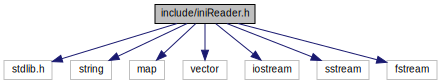
\includegraphics[width=350pt]{d4/d3d/iniReader_8h__incl}
\end{center}
\end{figure}
\-This graph shows which files directly or indirectly include this file\-:\nopagebreak
\begin{figure}[H]
\begin{center}
\leavevmode
\includegraphics[width=350pt]{df/d2a/iniReader_8h__dep__incl}
\end{center}
\end{figure}
\subsection*{\-Classes}
\begin{DoxyCompactItemize}
\item 
struct \hyperlink{structKeyRecord}{\-Key\-Record}
\begin{DoxyCompactList}\small\item\em \-Struct for holding a single settings key and its value. \end{DoxyCompactList}\item 
class \hyperlink{classINIReader}{\-I\-N\-I\-Reader}
\begin{DoxyCompactList}\small\item\em \-Class for parsing and storing contents of .ini files. \end{DoxyCompactList}\end{DoxyCompactItemize}
\subsection*{\-Defines}
\begin{DoxyCompactItemize}
\item 
\hypertarget{iniReader_8h_a18d295a837ac71add5578860b55e5502}{\#define {\bfseries \-S\-T\-R}(x)~\#x}\label{d5/dfd/iniReader_8h_a18d295a837ac71add5578860b55e5502}

\item 
\hypertarget{iniReader_8h_a31aad80d0a34263777a05e1f42e0884a}{\#define {\bfseries \-E\-X\-T\-R\-A\-C\-T}(type, sec, opt)~settings.\-extract\-Value$<$type$>$(\-S\-T\-R(sec),\-S\-T\-R(opt))}\label{d5/dfd/iniReader_8h_a31aad80d0a34263777a05e1f42e0884a}

\item 
\hypertarget{iniReader_8h_a6fb59ac401a769f7e35c027d4adf4a53}{\#define {\bfseries \-E\-X\-T\-R\-A\-C\-T\-P}(type, sec, opt)~settings-\/$>$extract\-Value$<$type$>$(\-S\-T\-R(sec),\-S\-T\-R(opt))}\label{d5/dfd/iniReader_8h_a6fb59ac401a769f7e35c027d4adf4a53}

\item 
\hypertarget{iniReader_8h_a235bb366e470c9fee24cc421a11751db}{\#define {\bfseries \-E\-X\-T\-R\-A\-C\-T\-\_\-}(obj, type, sec, opt)~settings.\-extract\-Value$<$type$>$(\-S\-T\-R(sec),\-S\-T\-R(opt))}\label{d5/dfd/iniReader_8h_a235bb366e470c9fee24cc421a11751db}

\item 
\hypertarget{iniReader_8h_ab6e8c0efe9fe69c5d46f21684ef555e5}{\#define {\bfseries \-E\-X\-T\-R\-A\-C\-T\-P\-\_\-}(obj, type, sec, opt)~settings-\/$>$extract\-Value$<$type$>$(\-S\-T\-R(sec),\-S\-T\-R(opt))}\label{d5/dfd/iniReader_8h_ab6e8c0efe9fe69c5d46f21684ef555e5}

\end{DoxyCompactItemize}
\subsection*{\-Typedefs}
\begin{DoxyCompactItemize}
\item 
\hypertarget{iniReader_8h_a47122fd58525bd1f2cbf2d640f6f6835}{typedef map$<$ string, \hyperlink{structKeyRecord}{\-Key\-Record} $>$ {\bfseries \-Key\-Map}}\label{d5/dfd/iniReader_8h_a47122fd58525bd1f2cbf2d640f6f6835}

\item 
\hypertarget{iniReader_8h_aadb294d991431880b3745d2c8ed5ef35}{typedef map$<$ string, \-Key\-Map $>$ {\bfseries \-Section\-Map}}\label{d5/dfd/iniReader_8h_aadb294d991431880b3745d2c8ed5ef35}

\item 
\hypertarget{iniReader_8h_ad48cd0136a0b83c26b8fcd49fcaff845}{typedef map$<$ string, string $>$ {\bfseries \-Default\-Key\-Map}}\label{d5/dfd/iniReader_8h_ad48cd0136a0b83c26b8fcd49fcaff845}

\item 
\hypertarget{iniReader_8h_af2cbef3947b8ab9a03975c47987430dd}{typedef map$<$ string, \*
\-Default\-Key\-Map $>$ {\bfseries \-Default\-Map}}\label{d5/dfd/iniReader_8h_af2cbef3947b8ab9a03975c47987430dd}

\end{DoxyCompactItemize}
\subsection*{\-Functions}
\begin{DoxyCompactItemize}
\item 
\hypertarget{iniReader_8h_a1f46f162d9c866fefee345b20ca9bcea}{{\bfseries \-\_\-\-\_\-attribute\-\_\-\-\_\-} ((unused)) static bool str\-Eq(const string \&s1}\label{d5/dfd/iniReader_8h_a1f46f162d9c866fefee345b20ca9bcea}

\end{DoxyCompactItemize}


\subsection{\-Detailed \-Description}

\hypertarget{mmu_8h}{\section{include/mmu.h \-File \-Reference}
\label{d2/df1/mmu_8h}\index{include/mmu.\-h@{include/mmu.\-h}}
}
{\ttfamily \#include $<$cassert$>$}\*
{\ttfamily \#include $<$string.\-h$>$}\*
{\ttfamily \#include $<$inttypes.\-h$>$}\*
{\ttfamily \#include \char`\"{}data\-\_\-structs.\-h\char`\"{}}\*
{\ttfamily \#include \char`\"{}ini\-Reader.\-h\char`\"{}}\*
\-Include dependency graph for mmu.\-h\-:\nopagebreak
\begin{figure}[H]
\begin{center}
\leavevmode
\includegraphics[width=350pt]{d4/da5/mmu_8h__incl}
\end{center}
\end{figure}
\-This graph shows which files directly or indirectly include this file\-:\nopagebreak
\begin{figure}[H]
\begin{center}
\leavevmode
\includegraphics[width=350pt]{dd/d98/mmu_8h__dep__incl}
\end{center}
\end{figure}
\subsection*{\-Classes}
\begin{DoxyCompactItemize}
\item 
struct \hyperlink{structsTLBE}{s\-T\-L\-B\-E}
\begin{DoxyCompactList}\small\item\em \-Struct representing a single entry in the \-T\-L\-B. \end{DoxyCompactList}\item 
class \hyperlink{classcMMU}{c\-M\-M\-U}
\begin{DoxyCompactList}\small\item\em \-Class representing an \-M\-M\-U in the \-C\-P\-U. \end{DoxyCompactList}\end{DoxyCompactItemize}
\subsection*{\-Enumerations}
\begin{DoxyCompactItemize}
\item 
enum \hyperlink{mmu_8h_ae08a7145dbbab15abf6cd31e4958d861}{e\-M\-M\-Ustate} \{ \hyperlink{mmu_8h_ae08a7145dbbab15abf6cd31e4958d861ab881282fb1f4def6fbeb85c4d6a2b34d}{\-M\-M\-U\-\_\-\-T\-H\-I\-T}, 
\hyperlink{mmu_8h_ae08a7145dbbab15abf6cd31e4958d861a38fa29ba4ff54aeb2233b2f1a0c31e8c}{\-M\-M\-U\-\_\-\-T\-M\-I\-S\-S}, 
\hyperlink{mmu_8h_ae08a7145dbbab15abf6cd31e4958d861ac0f58cca1cb5dc9e520cb453380cb06b}{\-M\-M\-U\-\_\-\-P\-F}
 \}
\begin{DoxyCompactList}\small\item\em \-State of the \-M\-M\-U after translation (or attempted) \end{DoxyCompactList}\end{DoxyCompactItemize}


\subsection{\-Detailed \-Description}


\subsection{\-Enumeration \-Type \-Documentation}
\hypertarget{mmu_8h_ae08a7145dbbab15abf6cd31e4958d861}{\index{mmu.\-h@{mmu.\-h}!e\-M\-M\-Ustate@{e\-M\-M\-Ustate}}
\index{e\-M\-M\-Ustate@{e\-M\-M\-Ustate}!mmu.h@{mmu.\-h}}
\subsubsection[{e\-M\-M\-Ustate}]{\setlength{\rightskip}{0pt plus 5cm}enum {\bf e\-M\-M\-Ustate}}}\label{d2/df1/mmu_8h_ae08a7145dbbab15abf6cd31e4958d861}
\begin{Desc}
\item[\-Enumerator\-: ]\par
\begin{description}
\index{\-M\-M\-U\-\_\-\-T\-H\-I\-T@{\-M\-M\-U\-\_\-\-T\-H\-I\-T}!mmu.\-h@{mmu.\-h}}\index{mmu.\-h@{mmu.\-h}!\-M\-M\-U\-\_\-\-T\-H\-I\-T@{\-M\-M\-U\-\_\-\-T\-H\-I\-T}}\item[{\em 
\hypertarget{mmu_8h_ae08a7145dbbab15abf6cd31e4958d861ab881282fb1f4def6fbeb85c4d6a2b34d}{\-M\-M\-U\-\_\-\-T\-H\-I\-T}\label{d2/df1/mmu_8h_ae08a7145dbbab15abf6cd31e4958d861ab881282fb1f4def6fbeb85c4d6a2b34d}
}]\-T\-L\-B \-Hit. \index{\-M\-M\-U\-\_\-\-T\-M\-I\-S\-S@{\-M\-M\-U\-\_\-\-T\-M\-I\-S\-S}!mmu.\-h@{mmu.\-h}}\index{mmu.\-h@{mmu.\-h}!\-M\-M\-U\-\_\-\-T\-M\-I\-S\-S@{\-M\-M\-U\-\_\-\-T\-M\-I\-S\-S}}\item[{\em 
\hypertarget{mmu_8h_ae08a7145dbbab15abf6cd31e4958d861a38fa29ba4ff54aeb2233b2f1a0c31e8c}{\-M\-M\-U\-\_\-\-T\-M\-I\-S\-S}\label{d2/df1/mmu_8h_ae08a7145dbbab15abf6cd31e4958d861a38fa29ba4ff54aeb2233b2f1a0c31e8c}
}]\-T\-L\-B \-Miss. \index{\-M\-M\-U\-\_\-\-P\-F@{\-M\-M\-U\-\_\-\-P\-F}!mmu.\-h@{mmu.\-h}}\index{mmu.\-h@{mmu.\-h}!\-M\-M\-U\-\_\-\-P\-F@{\-M\-M\-U\-\_\-\-P\-F}}\item[{\em 
\hypertarget{mmu_8h_ae08a7145dbbab15abf6cd31e4958d861ac0f58cca1cb5dc9e520cb453380cb06b}{\-M\-M\-U\-\_\-\-P\-F}\label{d2/df1/mmu_8h_ae08a7145dbbab15abf6cd31e4958d861ac0f58cca1cb5dc9e520cb453380cb06b}
}]\-Page \-Fault. \end{description}
\end{Desc}


\hypertarget{cleaningDaemon_8h}{\section{include/\-Policy/cleaning\-Daemon.h \-File \-Reference}
\label{de/d7e/cleaningDaemon_8h}\index{include/\-Policy/cleaning\-Daemon.\-h@{include/\-Policy/cleaning\-Daemon.\-h}}
}
{\ttfamily \#include \char`\"{}ini\-Reader.\-h\char`\"{}}\*
{\ttfamily \#include \char`\"{}\-Policy/frame\-Alloc.\-h\char`\"{}}\*
{\ttfamily \#include \char`\"{}vmm\-\_\-core.\-h\char`\"{}}\*
\-Include dependency graph for cleaning\-Daemon.\-h\-:\nopagebreak
\begin{figure}[H]
\begin{center}
\leavevmode
\includegraphics[width=350pt]{d9/d79/cleaningDaemon_8h__incl}
\end{center}
\end{figure}
\-This graph shows which files directly or indirectly include this file\-:\nopagebreak
\begin{figure}[H]
\begin{center}
\leavevmode
\includegraphics[width=350pt]{d5/dc5/cleaningDaemon_8h__dep__incl}
\end{center}
\end{figure}
\subsection*{\-Classes}
\begin{DoxyCompactItemize}
\item 
class \hyperlink{classcCleanDaemon}{c\-Clean\-Daemon}
\begin{DoxyCompactList}\small\item\em \-Cleaning \-Daemon for system. \end{DoxyCompactList}\end{DoxyCompactItemize}


\subsection{\-Detailed \-Description}

\hypertarget{pageReplace_8h}{\section{include/\-Policy/page\-Replace.h \-File \-Reference}
\label{d3/d2c/pageReplace_8h}\index{include/\-Policy/page\-Replace.\-h@{include/\-Policy/page\-Replace.\-h}}
}
{\ttfamily \#include \char`\"{}ini\-Reader.\-h\char`\"{}}\*
{\ttfamily \#include \char`\"{}utility/logger.\-h\char`\"{}}\*
{\ttfamily \#include \char`\"{}\-Policy/frame\-Alloc.\-h\char`\"{}}\*
\-Include dependency graph for page\-Replace.\-h\-:\nopagebreak
\begin{figure}[H]
\begin{center}
\leavevmode
\includegraphics[width=350pt]{d8/dd9/pageReplace_8h__incl}
\end{center}
\end{figure}
\-This graph shows which files directly or indirectly include this file\-:\nopagebreak
\begin{figure}[H]
\begin{center}
\leavevmode
\includegraphics[width=350pt]{de/daa/pageReplace_8h__dep__incl}
\end{center}
\end{figure}
\subsection*{\-Classes}
\begin{DoxyCompactItemize}
\item 
class \hyperlink{classcPRPolicy}{c\-P\-R\-Policy}
\begin{DoxyCompactList}\small\item\em \-Abstract \-Page \-Replacement \-Policy. \end{DoxyCompactList}\end{DoxyCompactItemize}
\subsection*{\-Enumerations}
\begin{DoxyCompactItemize}
\item 
enum \hyperlink{pageReplace_8h_af4bc4c41a44c2bd80e8cbf1aae370217}{e\-P\-R\-Status} \{ \hyperlink{pageReplace_8h_af4bc4c41a44c2bd80e8cbf1aae370217a743772bc7ef0bc5a46c4605f0c460c76}{\-P\-R\-\_\-\-S\-E\-R\-V\-I\-C\-E\-D}, 
\hyperlink{pageReplace_8h_af4bc4c41a44c2bd80e8cbf1aae370217a3937cd51db90fbe319ef9e8bb9bcc436}{\-P\-R\-\_\-\-S\-E\-R\-V\-I\-C\-E\-D\-\_\-\-I\-O}, 
\hyperlink{pageReplace_8h_af4bc4c41a44c2bd80e8cbf1aae370217a32dee3bb41068030734a88f443d04694}{\-P\-R\-\_\-\-N\-O\-\_\-\-A\-V\-A\-I\-L}, 
\hyperlink{pageReplace_8h_af4bc4c41a44c2bd80e8cbf1aae370217a7490bb9f71dbfea9c903f4a4b25288d4}{\-P\-R\-\_\-\-N\-O\-\_\-\-A\-C\-T\-I\-O\-N}
 \}
\end{DoxyCompactItemize}


\subsection{\-Detailed \-Description}


\subsection{\-Enumeration \-Type \-Documentation}
\hypertarget{pageReplace_8h_af4bc4c41a44c2bd80e8cbf1aae370217}{\index{page\-Replace.\-h@{page\-Replace.\-h}!e\-P\-R\-Status@{e\-P\-R\-Status}}
\index{e\-P\-R\-Status@{e\-P\-R\-Status}!pageReplace.h@{page\-Replace.\-h}}
\subsubsection[{e\-P\-R\-Status}]{\setlength{\rightskip}{0pt plus 5cm}enum {\bf e\-P\-R\-Status}}}\label{d3/d2c/pageReplace_8h_af4bc4c41a44c2bd80e8cbf1aae370217}
\begin{Desc}
\item[\-Enumerator\-: ]\par
\begin{description}
\index{\-P\-R\-\_\-\-S\-E\-R\-V\-I\-C\-E\-D@{\-P\-R\-\_\-\-S\-E\-R\-V\-I\-C\-E\-D}!page\-Replace.\-h@{page\-Replace.\-h}}\index{page\-Replace.\-h@{page\-Replace.\-h}!\-P\-R\-\_\-\-S\-E\-R\-V\-I\-C\-E\-D@{\-P\-R\-\_\-\-S\-E\-R\-V\-I\-C\-E\-D}}\item[{\em 
\hypertarget{pageReplace_8h_af4bc4c41a44c2bd80e8cbf1aae370217a743772bc7ef0bc5a46c4605f0c460c76}{\-P\-R\-\_\-\-S\-E\-R\-V\-I\-C\-E\-D}\label{d3/d2c/pageReplace_8h_af4bc4c41a44c2bd80e8cbf1aae370217a743772bc7ef0bc5a46c4605f0c460c76}
}]\-Page fault serviced. \index{\-P\-R\-\_\-\-S\-E\-R\-V\-I\-C\-E\-D\-\_\-\-I\-O@{\-P\-R\-\_\-\-S\-E\-R\-V\-I\-C\-E\-D\-\_\-\-I\-O}!page\-Replace.\-h@{page\-Replace.\-h}}\index{page\-Replace.\-h@{page\-Replace.\-h}!\-P\-R\-\_\-\-S\-E\-R\-V\-I\-C\-E\-D\-\_\-\-I\-O@{\-P\-R\-\_\-\-S\-E\-R\-V\-I\-C\-E\-D\-\_\-\-I\-O}}\item[{\em 
\hypertarget{pageReplace_8h_af4bc4c41a44c2bd80e8cbf1aae370217a3937cd51db90fbe319ef9e8bb9bcc436}{\-P\-R\-\_\-\-S\-E\-R\-V\-I\-C\-E\-D\-\_\-\-I\-O}\label{d3/d2c/pageReplace_8h_af4bc4c41a44c2bd80e8cbf1aae370217a3937cd51db90fbe319ef9e8bb9bcc436}
}]\-Page fault serviced with \-I/\-O required. \index{\-P\-R\-\_\-\-N\-O\-\_\-\-A\-V\-A\-I\-L@{\-P\-R\-\_\-\-N\-O\-\_\-\-A\-V\-A\-I\-L}!page\-Replace.\-h@{page\-Replace.\-h}}\index{page\-Replace.\-h@{page\-Replace.\-h}!\-P\-R\-\_\-\-N\-O\-\_\-\-A\-V\-A\-I\-L@{\-P\-R\-\_\-\-N\-O\-\_\-\-A\-V\-A\-I\-L}}\item[{\em 
\hypertarget{pageReplace_8h_af4bc4c41a44c2bd80e8cbf1aae370217a32dee3bb41068030734a88f443d04694}{\-P\-R\-\_\-\-N\-O\-\_\-\-A\-V\-A\-I\-L}\label{d3/d2c/pageReplace_8h_af4bc4c41a44c2bd80e8cbf1aae370217a32dee3bb41068030734a88f443d04694}
}]\-Page fault not serviced. \-No frames available (all pinned) \index{\-P\-R\-\_\-\-N\-O\-\_\-\-A\-C\-T\-I\-O\-N@{\-P\-R\-\_\-\-N\-O\-\_\-\-A\-C\-T\-I\-O\-N}!page\-Replace.\-h@{page\-Replace.\-h}}\index{page\-Replace.\-h@{page\-Replace.\-h}!\-P\-R\-\_\-\-N\-O\-\_\-\-A\-C\-T\-I\-O\-N@{\-P\-R\-\_\-\-N\-O\-\_\-\-A\-C\-T\-I\-O\-N}}\item[{\em 
\hypertarget{pageReplace_8h_af4bc4c41a44c2bd80e8cbf1aae370217a7490bb9f71dbfea9c903f4a4b25288d4}{\-P\-R\-\_\-\-N\-O\-\_\-\-A\-C\-T\-I\-O\-N}\label{d3/d2c/pageReplace_8h_af4bc4c41a44c2bd80e8cbf1aae370217a7490bb9f71dbfea9c903f4a4b25288d4}
}]\-Used in returning from circular page fault handler. \end{description}
\end{Desc}


\hypertarget{round__robin_8h}{\section{include/scheduler/round\-\_\-robin.h \-File \-Reference}
\label{d9/dd2/round__robin_8h}\index{include/scheduler/round\-\_\-robin.\-h@{include/scheduler/round\-\_\-robin.\-h}}
}
{\ttfamily \#include $<$assert.\-h$>$}\*
{\ttfamily \#include \char`\"{}scheduler/scheduler.\-h\char`\"{}}\*
\-Include dependency graph for round\-\_\-robin.\-h\-:\nopagebreak
\begin{figure}[H]
\begin{center}
\leavevmode
\includegraphics[width=350pt]{d4/d25/round__robin_8h__incl}
\end{center}
\end{figure}
\-This graph shows which files directly or indirectly include this file\-:\nopagebreak
\begin{figure}[H]
\begin{center}
\leavevmode
\includegraphics[width=242pt]{d2/d6c/round__robin_8h__dep__incl}
\end{center}
\end{figure}
\subsection*{\-Classes}
\begin{DoxyCompactItemize}
\item 
class \hyperlink{classcRoundRobin}{c\-Round\-Robin}
\begin{DoxyCompactList}\small\item\em \-Round \-Robin \-Scheduler. \end{DoxyCompactList}\item 
struct \hyperlink{structroundRobinInfo}{round\-Robin\-Info}
\begin{DoxyCompactList}\small\item\em \-Struct containing process info specific for \-Round-\/\-Robin scheduling. \end{DoxyCompactList}\end{DoxyCompactItemize}
\subsection*{\-Defines}
\begin{DoxyCompactItemize}
\item 
\hypertarget{round__robin_8h_a940ace0ba0421f4cd14c80411fb039e1}{\#define {\bfseries \-D\-E\-F\-\_\-\-B\-L\-O\-C\-K\-\_\-\-V\-E\-C\-\_\-\-S\-I\-Z\-E}~4}\label{d9/dd2/round__robin_8h_a940ace0ba0421f4cd14c80411fb039e1}

\item 
\hypertarget{round__robin_8h_abc4f0f9abea1b5443308e4ea84b52b21}{\#define {\bfseries \-Q\-U\-A\-N\-T\-U\-M}~4}\label{d9/dd2/round__robin_8h_abc4f0f9abea1b5443308e4ea84b52b21}

\end{DoxyCompactItemize}


\subsection{\-Detailed \-Description}

\hypertarget{id_8h}{\section{include/utility/id.h \-File \-Reference}
\label{df/db9/id_8h}\index{include/utility/id.\-h@{include/utility/id.\-h}}
}
{\ttfamily \#include $<$cstdio$>$}\*
{\ttfamily \#include $<$climits$>$}\*
{\ttfamily \#include $<$string$>$}\*
{\ttfamily \#include $<$queue$>$}\*
\-Include dependency graph for id.\-h\-:\nopagebreak
\begin{figure}[H]
\begin{center}
\leavevmode
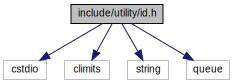
\includegraphics[width=305pt]{dc/dda/id_8h__incl}
\end{center}
\end{figure}
\-This graph shows which files directly or indirectly include this file\-:
\nopagebreak
\begin{figure}[H]
\begin{center}
\leavevmode
\includegraphics[width=350pt]{dd/ddf/id_8h__dep__incl}
\end{center}
\end{figure}
\subsection*{\-Classes}
\begin{DoxyCompactItemize}
\item 
class \hyperlink{classcIDManager}{c\-I\-D\-Manager}
\begin{DoxyCompactList}\small\item\em \-A class for managing unique \-I\-Ds. \end{DoxyCompactList}\end{DoxyCompactItemize}


\subsection{\-Detailed \-Description}

\hypertarget{logger_8h}{\section{include/utility/logger.h \-File \-Reference}
\label{d1/d8c/logger_8h}\index{include/utility/logger.\-h@{include/utility/logger.\-h}}
}
{\ttfamily \#include $<$assert.\-h$>$}\*
{\ttfamily \#include $<$iostream$>$}\*
{\ttfamily \#include $<$fstream$>$}\*
\-Include dependency graph for logger.\-h\-:\nopagebreak
\begin{figure}[H]
\begin{center}
\leavevmode
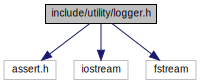
\includegraphics[width=272pt]{d6/db3/logger_8h__incl}
\end{center}
\end{figure}
\-This graph shows which files directly or indirectly include this file\-:
\nopagebreak
\begin{figure}[H]
\begin{center}
\leavevmode
\includegraphics[width=350pt]{d4/dcf/logger_8h__dep__incl}
\end{center}
\end{figure}
\subsection*{\-Functions}
\begin{DoxyCompactItemize}
\item 
\hypertarget{logger_8h_acf2f61176acdfe03ac9f73ec56fb3bd6}{\-F\-I\-L\-E $\ast$ \hyperlink{logger_8h_acf2f61176acdfe03ac9f73ec56fb3bd6}{init\-Log} (const char $\ast$filename)}\label{d1/d8c/logger_8h_acf2f61176acdfe03ac9f73ec56fb3bd6}

\begin{DoxyCompactList}\small\item\em \-Initialize a trace log at filename. \end{DoxyCompactList}\item 
\hypertarget{logger_8h_ac51ed3863a291e7293bea4c111ac8f9c}{void \hyperlink{logger_8h_ac51ed3863a291e7293bea4c111ac8f9c}{close\-Log} ()}\label{d1/d8c/logger_8h_ac51ed3863a291e7293bea4c111ac8f9c}

\begin{DoxyCompactList}\small\item\em \-Close the file stream for the trace log. \end{DoxyCompactList}\item 
\hypertarget{logger_8h_af756a6a1097f12014f446b298d8a266f}{\-F\-I\-L\-E $\ast$ \hyperlink{logger_8h_af756a6a1097f12014f446b298d8a266f}{get\-Stream} ()}\label{d1/d8c/logger_8h_af756a6a1097f12014f446b298d8a266f}

\begin{DoxyCompactList}\small\item\em \-Get the file stream to write to. \end{DoxyCompactList}\end{DoxyCompactItemize}


\subsection{\-Detailed \-Description}

\hypertarget{vmm__core_8h}{\section{include/vmm\-\_\-core.h \-File \-Reference}
\label{d4/d9a/vmm__core_8h}\index{include/vmm\-\_\-core.\-h@{include/vmm\-\_\-core.\-h}}
}
{\ttfamily \#include $<$ctime$>$}\*
{\ttfamily \#include $<$vector$>$}\*
{\ttfamily \#include $<$queue$>$}\*
{\ttfamily \#include $<$bitset$>$}\*
{\ttfamily \#include $<$string$>$}\*
{\ttfamily \#include $<$string.\-h$>$}\*
{\ttfamily \#include $<$inttypes.\-h$>$}\*
{\ttfamily \#include $<$sstream$>$}\*
{\ttfamily \#include $<$boost/dynamic\-\_\-bitset.\-hpp$>$}\*
{\ttfamily \#include \char`\"{}cpu.\-h\char`\"{}}\*
{\ttfamily \#include \char`\"{}data\-\_\-structs.\-h\char`\"{}}\*
{\ttfamily \#include \char`\"{}ini\-Reader.\-h\char`\"{}}\*
{\ttfamily \#include \char`\"{}exceptions.\-h\char`\"{}}\*
{\ttfamily \#include \char`\"{}round\-\_\-robin.\-h\char`\"{}}\*
{\ttfamily \#include \char`\"{}io\-\_\-control.\-h\char`\"{}}\*
{\ttfamily \#include \char`\"{}\-Policy/all\-P\-R.\-h\char`\"{}}\*
{\ttfamily \#include \char`\"{}utility/str\-Conv.\-h\char`\"{}}\*
{\ttfamily \#include \char`\"{}\-Policy/frame\-Alloc.\-h\char`\"{}}\*
{\ttfamily \#include \char`\"{}\-Policy/cleaning\-Daemon.\-h\char`\"{}}\*
\-Include dependency graph for vmm\-\_\-core.\-h\-:\nopagebreak
\begin{figure}[H]
\begin{center}
\leavevmode
\includegraphics[width=350pt]{d3/d13/vmm__core_8h__incl}
\end{center}
\end{figure}
\-This graph shows which files directly or indirectly include this file\-:\nopagebreak
\begin{figure}[H]
\begin{center}
\leavevmode
\includegraphics[width=350pt]{d1/df7/vmm__core_8h__dep__incl}
\end{center}
\end{figure}
\subsection*{\-Classes}
\begin{DoxyCompactItemize}
\item 
class \hyperlink{classcVMM}{c\-V\-M\-M}
\begin{DoxyCompactList}\small\item\em \-Virtual \-Memory \-Manager core class. \end{DoxyCompactList}\end{DoxyCompactItemize}
\subsection*{\-Variables}
\begin{DoxyCompactItemize}
\item 
\hypertarget{vmm__core_8h_a5b3dc30d8a7fc0f65a8e563cba9654cc}{\hyperlink{classINIReader}{\-I\-N\-I\-Reader} $\ast$ {\bfseries settings}}\label{d4/d9a/vmm__core_8h_a5b3dc30d8a7fc0f65a8e563cba9654cc}

\end{DoxyCompactItemize}


\subsection{\-Detailed \-Description}

\printindex
\end{document}
